\documentclass[12pt,letterpaper,oneside]{book}
\usepackage[top=1in, bottom=1in, left=1.25in, right=1in, footskip=0.25in]{geometry}
\usepackage{fancyhdr}

\fancypagestyle{frontmatter}{%
  \renewcommand{\headrulewidth}{0pt}% No header rule
  \renewcommand{\footrulewidth}{0pt}% No footer rule
  \fancyhf{}% Clear header/footer
  \fancyfoot[C]{\thepage}%
}

\fancypagestyle{mainmatter}{%
  \renewcommand{\headrulewidth}{0.4pt}% header rule
  \fancyhf{}
  \fancyhead[L]{\itshape\nouppercase{\leftmark}}
  \fancyfoot[C]{\thepage}
}

\usepackage[font=rm, labelfont={rm,bf}, margin=1cm]{caption}
\usepackage[T1]{fontenc}
\usepackage{textcomp}
\usepackage{lmodern}
\usepackage[english]{babel}
\usepackage[utf8x]{inputenc}
\usepackage[sc]{mathpazo}
\usepackage{amsmath,amssymb,amsfonts,mathrsfs,mathtools}
\usepackage{graphicx}
\usepackage[square,sort,comma,numbers]{natbib}
\usepackage{setspace}
\usepackage{titling}
\usepackage{bibentry}
\usepackage[plain]{fancyref}
\usepackage[linktoc=all]{hyperref}
\hypersetup{
    colorlinks,
    citecolor=black,
    filecolor=black,
    linkcolor=black,
    urlcolor=black
}

% For figure captions
\providecommand{\titlecaption}[2]{\caption[#1]{{\bf #1.} #2}}

% For dummy text
\usepackage{blindtext}


% Imports/macros for chapter 2
\usepackage{booktabs}
% \usepackage{chemarr}
\usepackage{longtable}

% Imports/macros for chapter 3
\usepackage{siunitx}
%\providecommand{\num}[1]{#1}  % Change this for the final compile

\providecommand{\bm}[1]{\mathbf{#1}}
\providecommand{\zdata}{\ensuremath{\hat{\bm x}}}
\providecommand{\zspline}{\ensuremath{\tilde{\bm x}}}
\providecommand{\zopt}{\ensuremath{{\bm x}^\star}}
\providecommand{\popt}{\ensuremath{{\bm p}^\star}}

% Imports for chapter 5
\usepackage{nicefrac}
\usepackage{supertabular}

% For model float
\usepackage{float}
\newfloat{model}{thp}{lop}[chapter]
\floatname{model}{Model}
\floatstyle{plaintop}
\restylefloat{model}

% For list of models in the preamble
% \usepackage{scrhack} % load after "float"

\newcommand*{\fancyrefmodlabelprefix}{mod}

\fancyrefaddcaptions{english}{%
  \providecommand*{\frefmodname}{model}%
  \providecommand*{\Frefmodname}{Model}%
}

\frefformat{plain}{\fancyrefmodlabelprefix}{\frefmodname\fancyrefdefaultspacing#1}
\Frefformat{plain}{\fancyrefmodlabelprefix}{\Frefmodname\fancyrefdefaultspacing#1}

\frefformat{vario}{\fancyrefmodlabelprefix}{%
  \frefmodname\fancyrefdefaultspacing#1#3%
}
\Frefformat{vario}{\fancyrefmodlabelprefix}{%
  \Frefmodname\fancyrefdefaultspacing#1#3%
}

\title{Mathematical Approaches to Understanding Mammalian Circadian Rhythms}

\begin{document}
\doublespace
\frontmatter
\pagestyle{mainmatter}
\thispagestyle{empty}
\begin{center}
  UNIVERSITY OF CALIFORNIA\\
  Santa Barbara\\
  \vfil
  {\Large\thetitle}\\
  \vfil
  by\\
  \vfil
  {\large Peter Corbin\ St.\ John}\\
  \vfil
  Committee in charge:\\
  Professor Francis J. Doyle III, Chair\\
  Professor Samir Mitragotri\\
  Professor Michelle A. O'Malley\\
  Professor Linda R. Petzold\\
  \vfil
  June 2015
\end{center}

\thispagestyle{empty}
The dissertation of Peter C. St. John is approved.
\vfil
\begin{minipage}{0.6\textwidth}
  \rule{\textwidth}{0.7pt}
  {\sc Samir Mitragotri}
\end{minipage}
\hfill
\begin{minipage}{0.3\textwidth}
  \rule{\textwidth}{0.7pt}
  {\sc Date}
\end{minipage}

\vfil
\begin{minipage}{0.6\textwidth}
  \rule{\textwidth}{0.7pt}
  {\sc Michelle A. O'Malley}
\end{minipage}
\hfill
\begin{minipage}{0.3\textwidth}
  \rule{\textwidth}{0.7pt}
  {\sc Date}
\end{minipage}

\vfil
\begin{minipage}{0.6\textwidth}
  \rule{\textwidth}{0.7pt}
  {\sc Linda R. Petzold}
\end{minipage}
\hfill
\begin{minipage}{0.3\textwidth}
  \rule{\textwidth}{0.7pt}
  {\sc Date}
\end{minipage}

\vfil
\begin{minipage}{0.6\textwidth}
  \rule{\textwidth}{0.7pt}
  {\sc Francis J. Doyle III, Committee Chair}
\end{minipage}
\hfill
\begin{minipage}{0.3\textwidth}
  \rule{\textwidth}{0.7pt}
  {\sc Date}
\end{minipage}


\chapter*{}
\null
\vfill
\begin{center}
  \thetitle\\[2ex]
  Copyright \copyright \ 2015\\
  by\\
  Peter C. St. John
\end{center}

% \chapter*{Acknowledgement}
\markboth{Acknowledgement}{Acknowledgement}

{\singlespace

First and foremost, I would like to think Frank Doyle III for taking the time to advise me and for providing numerous opportunities for me to present my research at conferences.
I also thank the other members of my PhD thesis committee for their continued support and encouragement: Samir Mitragotri and Michelle O'Malley for keeping my work biologically relevant; and Linda Petzold for her expertise in numerical methods.
I would also like to thank Linda for her excellent class in ODE integration, which greatly helped me understand and appreciate the algorithms I had largely taken for granted.

I would also like to thank the past and current members of the Doyle group, who have made my past five years so memorable.
In no particular order, I thank Stephanie Taylor, for while we didn't actually overlap at UCSB, she nevertheless provided constant guidance and suggestions on the various manuscripts and presentations I prepared during my PhD thesis.
I also thank Bharath Ananthasubramaniam and Panagiota (Pegy) Foteinou for their help getting me started when I first joined the groups and for many excellent lunchtime conversations.
I also thank John Abel for his overall enthusiasm and specifically his help with stochastic methods, without which I may have taken a different path for my last two papers.
I should not forget group members who have worked on other projects: Ravi Gondhalekar, Yongqiang Wang, and Felipe N\'{u}\~{n}ez, who graciously put up with my constant questions about spectral analysis and analytical methods.

I would also like to thank my fianc\'{e}e Katherine LeVan - first in a professional context, for her depth of knowledge of classical statistics and assistance with many aspects of my research.
Most importantly, of course, I thank her for her endless patience and support. 
Similarly, I thank my parents and brother, Christopher, for always being there when I need them.

Finally, I thank the various funding sources who have made this project possible.
Most importantly, I appreciate the generous fellowship given to me by the Mitsubishi Chemical Corporation, which has given me the freedom to pursue whichever project caught my enthusiasm.
I also thank financial support from the National Institutes of Health/National Institute of General Medical Sciences under award number 1R01GM096873-01 and from the Institute for Collaborative Biotechnologies through grant W911NF-09-0001 from the U.S.\ Army Research Office.

}

%Previous group members - Bharath, Stephanie, Pegy, John
%Family
%Money (include Mitsubishi)

% \Blindtext

{
\singlespace
\setlength{\parindent}{0em}
\setlength{\parskip}{1em}

\section*{Vita of Peter C. St. John}

\subsection*{Contact Information}
\vspace{.05in}
\begin{tabular}{@{}p{3.5in}p{4in}}
Department of Chemical Engineering   & {\it Phone:}  (508) 494-2474\\             
University of California, Santa Barbara & {\it E-mail:} pstjohn@engineering.ucsb.edu\\       
Santa Barbara, CA 93106-5080 & {\it Office:} Engineering II, Rm. 1508\\
\end{tabular}


\subsection*{Education}
  {\bf University of California, Santa Barbara} \hfill {\bf September 2010 - present} \\
  {\em Ph.D. Candidate, Department of Chemical Engineering} \hfill Santa Barbara,
  California \\[-3ex]
  % \begin{itemize}
  % \item Advisor:  Francis J. Doyle III
  % \item GPA: 3.68
  % \end{itemize}

  {\bf Tufts University}  \hfill {\bf September 2006 - May 2010}\\
  {\em BS, Chemical and Biological Engineering} \hfill Medford,
  Massachusetts\\[-3ex]
  % \begin{itemize}
  % \item Summa Cum Laude, Thesis Honors, Dean's List every semester
  % \item GPA: 3.79
  % \end{itemize}

\subsection*{Honors and Awards} 
CAST Student Travel Grant \hfill {\bfseries September 2014}\\
Society for Research on Biological Rhythms (SRBR) Research Merit Award \hfill {\bf June 2014}\\
Best Poster, Center for Chronobiology Symposium, UCSD \hfill {\bf February 2014} \\
$1^\textrm{st}$ Place, SRBR Logo Competition \hfill {\bf January 2014} \\
Mitsubishi Chemical Fellowship Recipient \hfill {\bf 2012-2015} \\
UCSB Scienceline 2011-2012 Life Science Outstanding Answerer \hfill {\bf June 2012} \\
National Science Foundation GRFP Honorable Mention \hfill {\bf April 2011} \\
Class of 1947 Victor Prather Prize \hfill {\bf May 2010}\\
Max Tischler Prize Scholarship \hfill  {\bf May 2009}\\
Elected to Tau Beta Pi \hfill  {\bf September 2008}\\

\subsection*{Publications}
{\bfseries St.\ John, P.C.,} Taylor, S.R., Abel, J.H., and F.J. Doyle III. Amplitude metrics for cellular circadian bioluminescence reporters (2014) {\itshape Biophysical Journal}, 107 (11) pp. 2712-2722

{\bfseries St.\ John, P.C.,} Hirota, T., Kay, S.A. and F.J. Doyle III.
Spatiotemporal separation of PER and CRY posttranslational regulation in the
mammalian circadian clock (2014) {\itshape PNAS}, 111 (5) pp. 2040-2045.

Yang, R., Rodriguez-Fernandez, M., {\bfseries St.\ John, P.C.,} and F.J. Doyle III. Chapter 8 -- Systems Biology (2014) In E. Carson and C. Cobelli (Eds.)
{\itshape Modelling Methodology for Physiology and Medicine, 2nd Edition}, pp.
159-187.

{\bfseries St.\ John, P.C.,} and F.J. Doyle III. Estimating confidence intervals in predicted responses for oscillatory biological models (2013) {\itshape BMC Systems Biology} 7:71.
 
Hirota, T., Lee, J.W., {\bfseries St.\ John, P.C.}, Sawa, M., Iwaisako, K.,
Noguchi, T., Pongsawakul, P.Y., Sonntag, T., Welsh, D.K., Brenner, D.A., Doyle,
F.J. III, Schultz, P.G., Kay, S.A.,  Identification of small molecule
activators of cryptochrome (2012) {\itshape Science}, 337 (6098) pp. 1094-1097.

Murphy A.R., {\bf St.\ John P.C.}, Kaplan D.L. Modification of silk fibroin using diazonium coupling chemistry and the effects on hMSC proliferation and differentiation (2008) {\em Biomaterials}, 29 (19), pp. 2829-2838.  

\subsection*{Contributed Talks}
{\bfseries St.\ John, P.C.,} and F.J. Doyle III. November 2014. Development of Amplitude Response Curves for Single-Cell and Population-Level Circadian Systems. {\itshape To be presented} at the 2014 AIChE Annual Meeting, Atlanta, GA

% {\bfseries St.\ John, P.C.} October 2014. \textit{Mitsubishi Lecture:} Mathematical approaches to understanding amplitude in mammalian circadian rhythms. Presented at the $7^{\mathrm{th}}$ Annual Clorox-Amgen Graduate Student Symposium, Santa Barbara, CA.

{\bfseries St.\ John, P.C.,} and F.J. Doyle III. June 2014. Amplitude metrics for uncoupled cellular circadian bioluminescence reporters. Presented at the Society for Research on Biological Rhythms Meeting, Big Sky, MT.

{\bfseries St.\ John, P.C.,} and F.J. Doyle III. October 2012. Cryptochrome balancing for period control: mathematical insights into circadian clock design. Presented at the Model-based Analysis and Control of Cellular Processes Workshop, Purdue University, West Lafayette, IN.

\subsection*{Poster Presentations}
{\bfseries St.\ John, P.C.,} and F.J. Doyle III. February 2014. Spatiotemporal
separation of PER and CRY post-translation regulation. Presented at the UCSD
Center for Chronobiology Symposium, La Jolla, CA.

{\bfseries St.\ John, P.C.,} T. Hirota, S.A. Kay, and F.J. Doyle III. July 2013. Estimating confidence intervals in model predictions to determine plausible mechanisms for small molecule modifiers. Presented at the Chronobiology Gordon Research Conference, Newport, RI.

{\bfseries St.\ John, P.C.,} and F.J. Doyle III. February 2013. Predictive confidence intervals from mathematical circadian models. Presented at the UCSD Center for Chronobiology Symposium, La Jolla, CA.

% {\bfseries St.\ John, P.C.,} and F.J. Doyle III. October 2012. Modeling of circadian rhythms for small molecule modulator characterization. Presented at the Amgen-Clorox Graduate Student Symposium, Santa Barbara, CA.

{\bfseries St.\ John, P.C.,} T. Hirota, S. Kay, and F.J. Doyle III. May 2012. Cryptochrome balancing for period control. Presented at the Meeting of the Society for Research on Biological Rhythms, Destin, FL.

{\bfseries St.\ John, P.C.,} and F.J. Doyle III. February 2012. Perturbation analysis of circadian clock degradation. Presented at the UCSD Center for Chronobiology Symposium, La Jolla, CA.

{\bfseries St.\ John, P.C.,} M. Rodriguez-Fernandez, and F.J. Doyle III.  June 2011. Advanced global optimization and sensitivity techniques for analyzing deterministic circadian models. Presented at the 12th Annual UC Systemwide Bioengineering Symposium, Santa Barbara, CA.

% {\bfseries St.\ John, P.C.,} and F.J. Doyle III. September 2011. Perturbation analysis of circadian clock function. Presented at the Amgen-Clorox Graduate Student Symposium, Santa Barbara, CA.

% {\bfseries St.\ John, P.C.,} J. A. Hanson, and T. J. Deming. August 2009. Release from Nanoscale Water-in-Oil-in-Water Double Emulsions Stabilized by Block Copolypeptide Surfactants. Presented at the UCLA NanoCER Poster Session, Los Angeles, CA.

% {\bfseries St.\ John, P.C.,} and H. Yi. April 2008. Catalytic hydrodechlorination of 2-chlorophenol using viral-templated palladium nanoparticles. Presented at the 10th Annual Undergraduate Research and Scholarship Symposium, Medford MA.


\subsection*{Seminars}
{\bfseries St.\ John, P.C.} May 2013. Sensitivity analysis in the study of
mammalian circadian rhythms. Presented at the UCSB NSF-IGERT systems biology
seminar series, Santa Barbara, CA.

\subsection*{Research Experience}

{\bf University of California, Santa Barbara} \hfill {\bf September 2010 - present}\\
{\em Ph.D. Candidate} \hfill Santa Barbara, California\\
Computational analysis of the mammalian circadian clock, with a focus on
elucidating the functional design consequences of the underlying genetic
regulatory network.\\
% This work deals primarily with simulating biological
% networks as systems of coupled, nonlinear, deterministic ordinary differential
% equations.\\
Advisor: Francis J. Doyle III \\
Department: Chemical Engineering

{\bf Tufts University} \hfill {\bf September 2009 - May 2010}\\
{\em Senior Honors Thesis} \hfill Medford, Massachusetts\\
Catalytic Hydrodechlorination of 2-Chlorophenol using Viral-templated Palladium Nanoparticles\\
Advisor: Hyunmin Yi \\
Department: Chemical and Biological Engineering

{\bf University of California, Los Angeles} \hfill {\bf June 2009 - August 2009}\\
{\em UCLA NanoCER Program (NSF REU)} \hfill Los Angeles, California\\
Encapsulation Efficiencies and Release Rates from Water-in-Oil-in-Water Nanoemulsions\\
Advisor: Timothy Deming\\
Department: Bioengineering

{\bf Tufts University} \hfill {\bf June 2008 - August 2008}\\
{\em Tufts Summer Scholars} \hfill Medford, Massachusetts\\
Hydrodechlorination of 2-Chlorophenol with Palladium Nanoparticles on Genetically Modified Tobacco Mosaic Virus Scaffolds\\
Advisor: Hyunmin Yi\\
Department: Chemical and Biological Engineering

{\bf Tufts University} \hfill {\bf October 2007 - May 2008}\\
{\em Undergraduate Research Credit} \hfill Medford, Massachusetts\\
Chemically Modified Silk Fibroin Based Scaffolds for Bone Tissue Engineering\\
Advisor: David Kaplan\\
Department: Biomedical Engineering

\subsection*{Teaching Experience}
%132c again
{\bf University of California, Santa Barbara}  \hfill {\bf January 2013 -
  December 2013}\\
{\em Teaching Assistant, ChE132c}\hfill  Santa Barbara, California\\
Helped teach undergraduate statistics for two subsequent years: gave three
lectures, held office hours and review sessions, and graded homeworks.

{\bf University of California, Santa Barbara} \hfill {\bf March 2012 - June 2012}\\
{\em Teaching Assistant, ChE180a}\hfill  Santa Barbara, California\\
Designed and ran experiments for the junior laboratory course. Also helped in grading student reports.

\subsection*{Community Involvement}
{\bf Peer Review \hfill January 2014-present}\\
Reviewer for Biophysical Journal;  IEEE Control Systems Society Conference; 21st International Symposium on
Mathematical Theory of Networks and Systems

{\bf Scienceline ``Ask A Scientist"} \hfill {\bf December 2010 - present}\\
Answers science and engineering questions posed by students and teachers from local K-12 schools. \\
{\bfseries Website:} www.scienceline.ucsb.edu

{\bf UCSB Discover Engineering Weekend} \hfill {\bf May 2011}\\
Helped organize and run a weekend for local high school students to learn basic engineering principles and apply their knowledge to build miniature alternative energy cars.

% \subsection*{Leadership Experiences}
% {\bf Tufts Chapter of the AIChE}\\
% {\em Vice President} \hfill {\bf September 2008 - May 2010}\\
% (American Institute of Chemical Engineers) Coordinated department-wide social, professional, and community service events

\subsection*{Mentoring Experience}
Amanda Luan, Undergraduate Student, ICB SSB URAP \hfill {\bf June 2014 - December 2014} \\
Lukas Widmer, Masters Student, ETH Zurich \hfill {\bf April 2012 - February 2013} \\
Andrew Barisser, Rotation Student, BMSE UCSB \hfill {\bf September 2012 - December 2012}

}

% \chapter*{Abstract}
\markboth{Abstract}{Abstract}

\Blindtext

% Daily changes in mammalian physiology, known as circadian rhythms, are coordinated by intricate genetic regulatory networks that process information from the environment to prepare the body for upcoming demands. This natural feed-forward controller is essential to maintaining metabolic homeostasis, and compromised circadian rhythms have been linked to the onset of metabolic disease. Since circadian rhythms can be damped by factors such as jet lag, shift work, and high fat diets, numerous studies have focused on elucidating mechanisms which govern circadian amplitude. My work uses techniques from dynamic systems to model circadian oscillations at different scales. By capturing changes in gene expression using ordinary differential equation models, I am able to investigate how pharmacological changes affect gene expression at the single-cell level. However, physiologically relevant changes gene expression are determined by the collective output of many cells at the tissue-level.  I therefore develop computationally efficient techniques of simulating the average response from a population of oscillating cells. These techniques use a probability density function to describe the synchrony of the population, and a convection-diffusion equation to capture the evolution of the population in time. My work provides new tools to help understand the effects of pharmacological perturbations in experimental conditions, which will ultimately allow the development of therapies to treat common health issues associated with the demands of a 24-hr society.

\tableofcontents
\listoffigures
\listof{model}{List of Models}
\listoftables

\mainmatter
\chapter{Introduction}
Since life's first beginnings, nature has been seeking optimal solutions to surviving in a constantly changing environment.
One key adaptation towards this goal, as evidenced by the ubiquity with which it is found throughout the tree of life, is the ability of an organism to anticipate daily changes to its environment.
Such rhythms are known as {\itshape circadian}, and are classified by a number of defining characteristics \cite{Dunlap2009}:

\begin{itemize}
  \item They are {\em endogenous}, meaning they continue to oscillate even when the organism is isolated from its environment.

  \item They are temperature compensated, maintaining a consistent period for moderate changes in average temperature.

  \item They are {\em entrainable}, meaning they can adjust their phase and period in response to a changing in environmental signal.

  \item They oscillate with a roughly 24 hour period.
\end{itemize}

In this thesis, we apply techniques from systems biology in order to gain a more thorough understanding of how circadian rhythms control mammalian physiology, and how these rhythms might be altered through pharmacological therapies. % Really for abstract
Systems biology is a multidisciplinary field, drawing from biology, mathematics, and computer science. 
In this chapter, we first provide a background on the biology of circadian rhythms, followed by an introduction to the mathematical techniques which have been used to study them. 
We discuss some computational considerations in the estimation of model parameters.

\section{Biological background}

\subsection{Dynamics of gene expression}

In the central dogma of molecular biology, genetic information is passed from DNA to mRNA to protein. 
While each cell in a multi-celled organism contains nearly identical DNA, the rate with which different genes are expressed results in substantial differences in cell type and function. 
These differences are the result of complex gene transcription networks, in which the production of some proteins - known as transcription factors - activate or repress the production of other genes. 
Similar to electrical circuits, network motifs such as positive and negative feedback arise from the interconnection of transcription factors.

Gene regulatory networks are essential to biological function. 
Cells maintain energy homeostasis by carefully balancing the flux of metabolites into energy storage and energy production pathways. 
These reactions are catalyzed by numerous enzymes, the activities of which must fluctuate to ensure the proper allocation of resources within a cell.
Enzyme production, degradation, and activation are controlled by transcription factors, and thus environmental conditions can be processed by complex network interactions to regulate metabolic function.
Circadian rhythms play a major role in the regulation of metabolic cycles, as periodic shifts in energy availability require a similar periodic shifts in gene transcription.



\subsection{Evolutionary history}

By looking at the evolutionary history of circadian rhythms, Edgar and colleges \cite{Edgar2012} demonstrated that cellular timekeeping may have began as a response to the Great Oxidation Event occurring $\approx 2.5$ billion years ago. 
Due to increased oxygen levels, the generation of reactive oxygen species in the cell can lead to oxidation of key biomolecules, prompting cells to express scavenging mechanisms during times of high UV light exposure. 
Over time, these pathways coupled to transcription-translation feedback loops in individual organisms, giving rise to a diverse set of circadian regulatory pathways (\fref{fig:edgarros}, from \cite{Edgar2012}). 

\begin{figure}[tbp]
  \centering
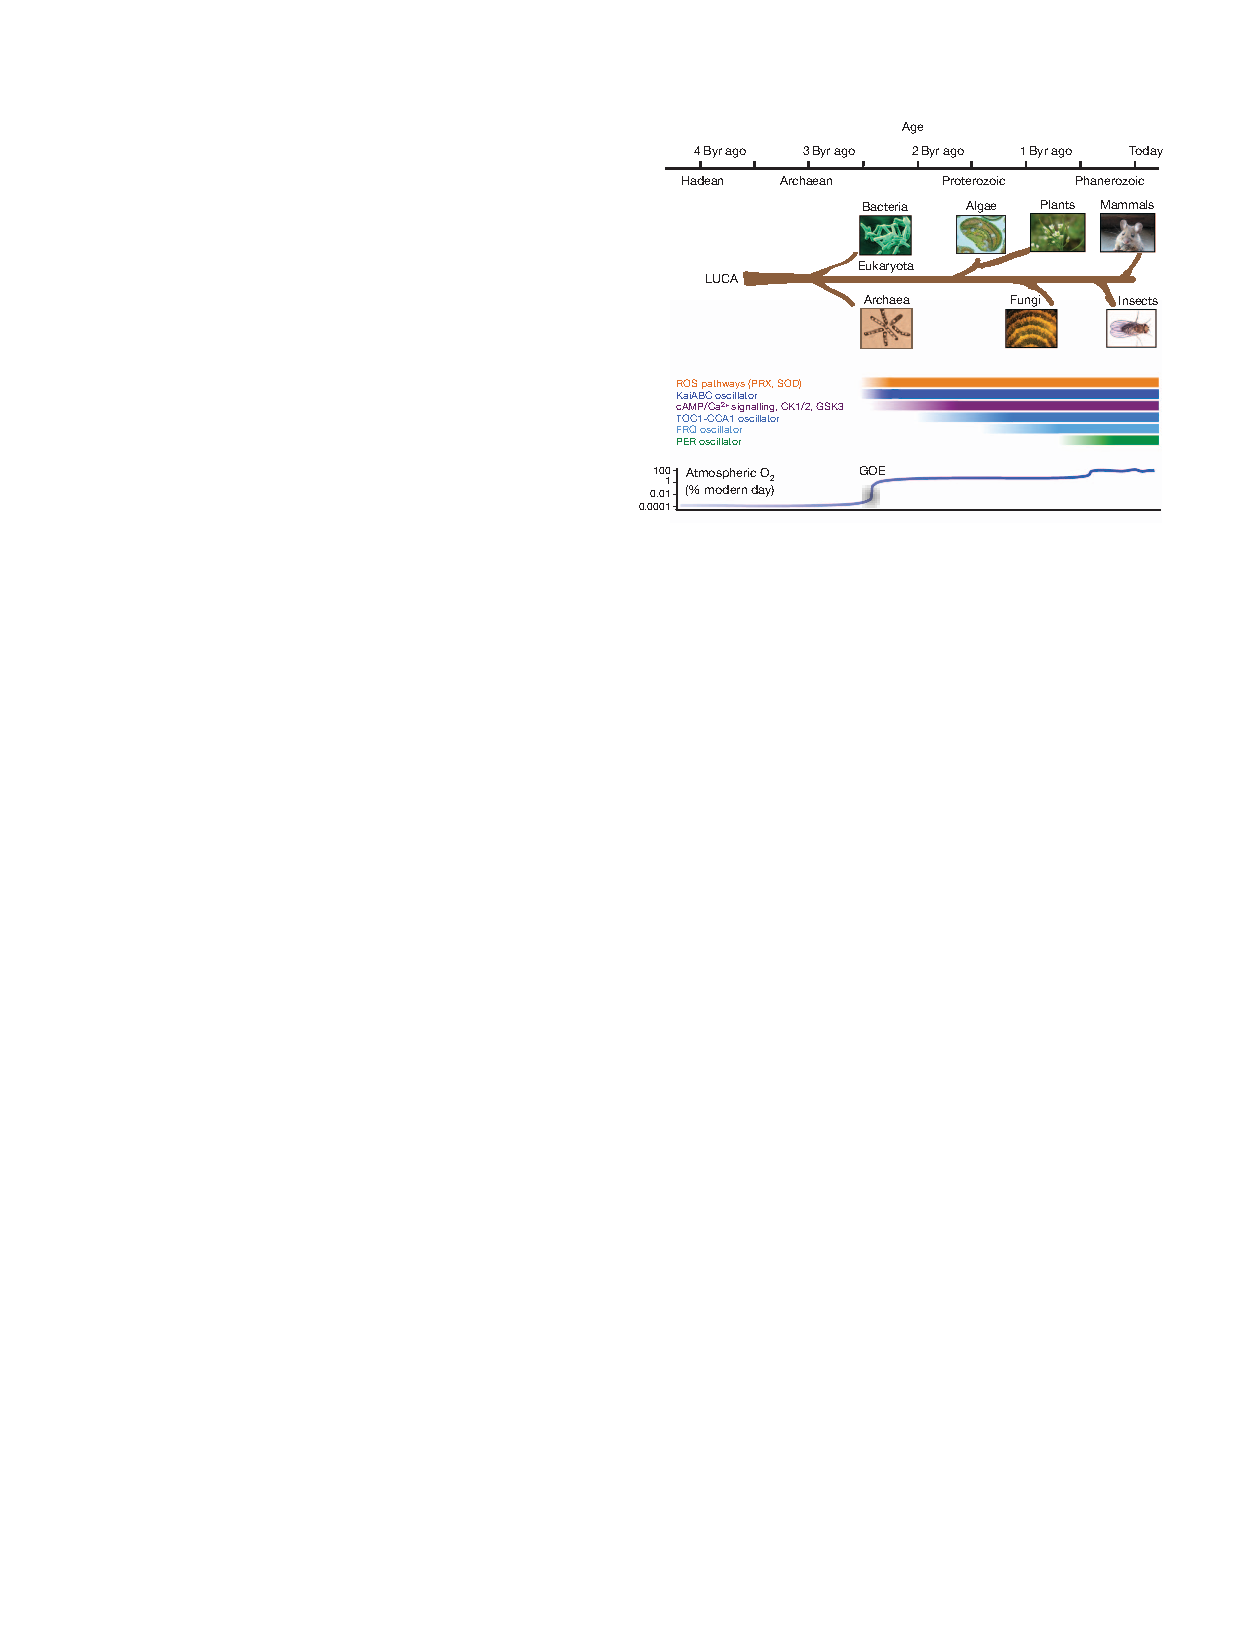
\includegraphics[width=0.8\textwidth]{chap1/figures/edgar_ros.pdf}
\titlecaption{Reactive oxygen species are conserved markers of circadian rhythms}{A timeline of the appearance of the main circadian feedback loops demonstrates that the rhythmic protection against light-mediated oxidation is a conserved rhythm across many evolutionary trees. Figure reprinted from \cite{Edgar2012}.}
  \label{fig:edgarros}
\end{figure}

\subsection{Circadian rhythms in mammals}

\subsubsection{Tissue-level clocks}

In mammals, circadian rhythms are organized in a hierarchical structure, in which inputs from the environment are processed separately by different tissue-level clocks (\fref{fig:feedforward}). 
Light, the primary entraining factor, is directed towards the suprachiasmatic nucleus (SCN), a tissue in the brain that serves as the body's master pacemaker \cite{Ralph1990}. 
In the SCN, approximately $20,000$ cells communicate via intercellular coupling to determine a precise internal time, which coordinates rhythms in locomotor activity \cite{Aton2005}.

\begin{figure}[tbp]
  \centering
  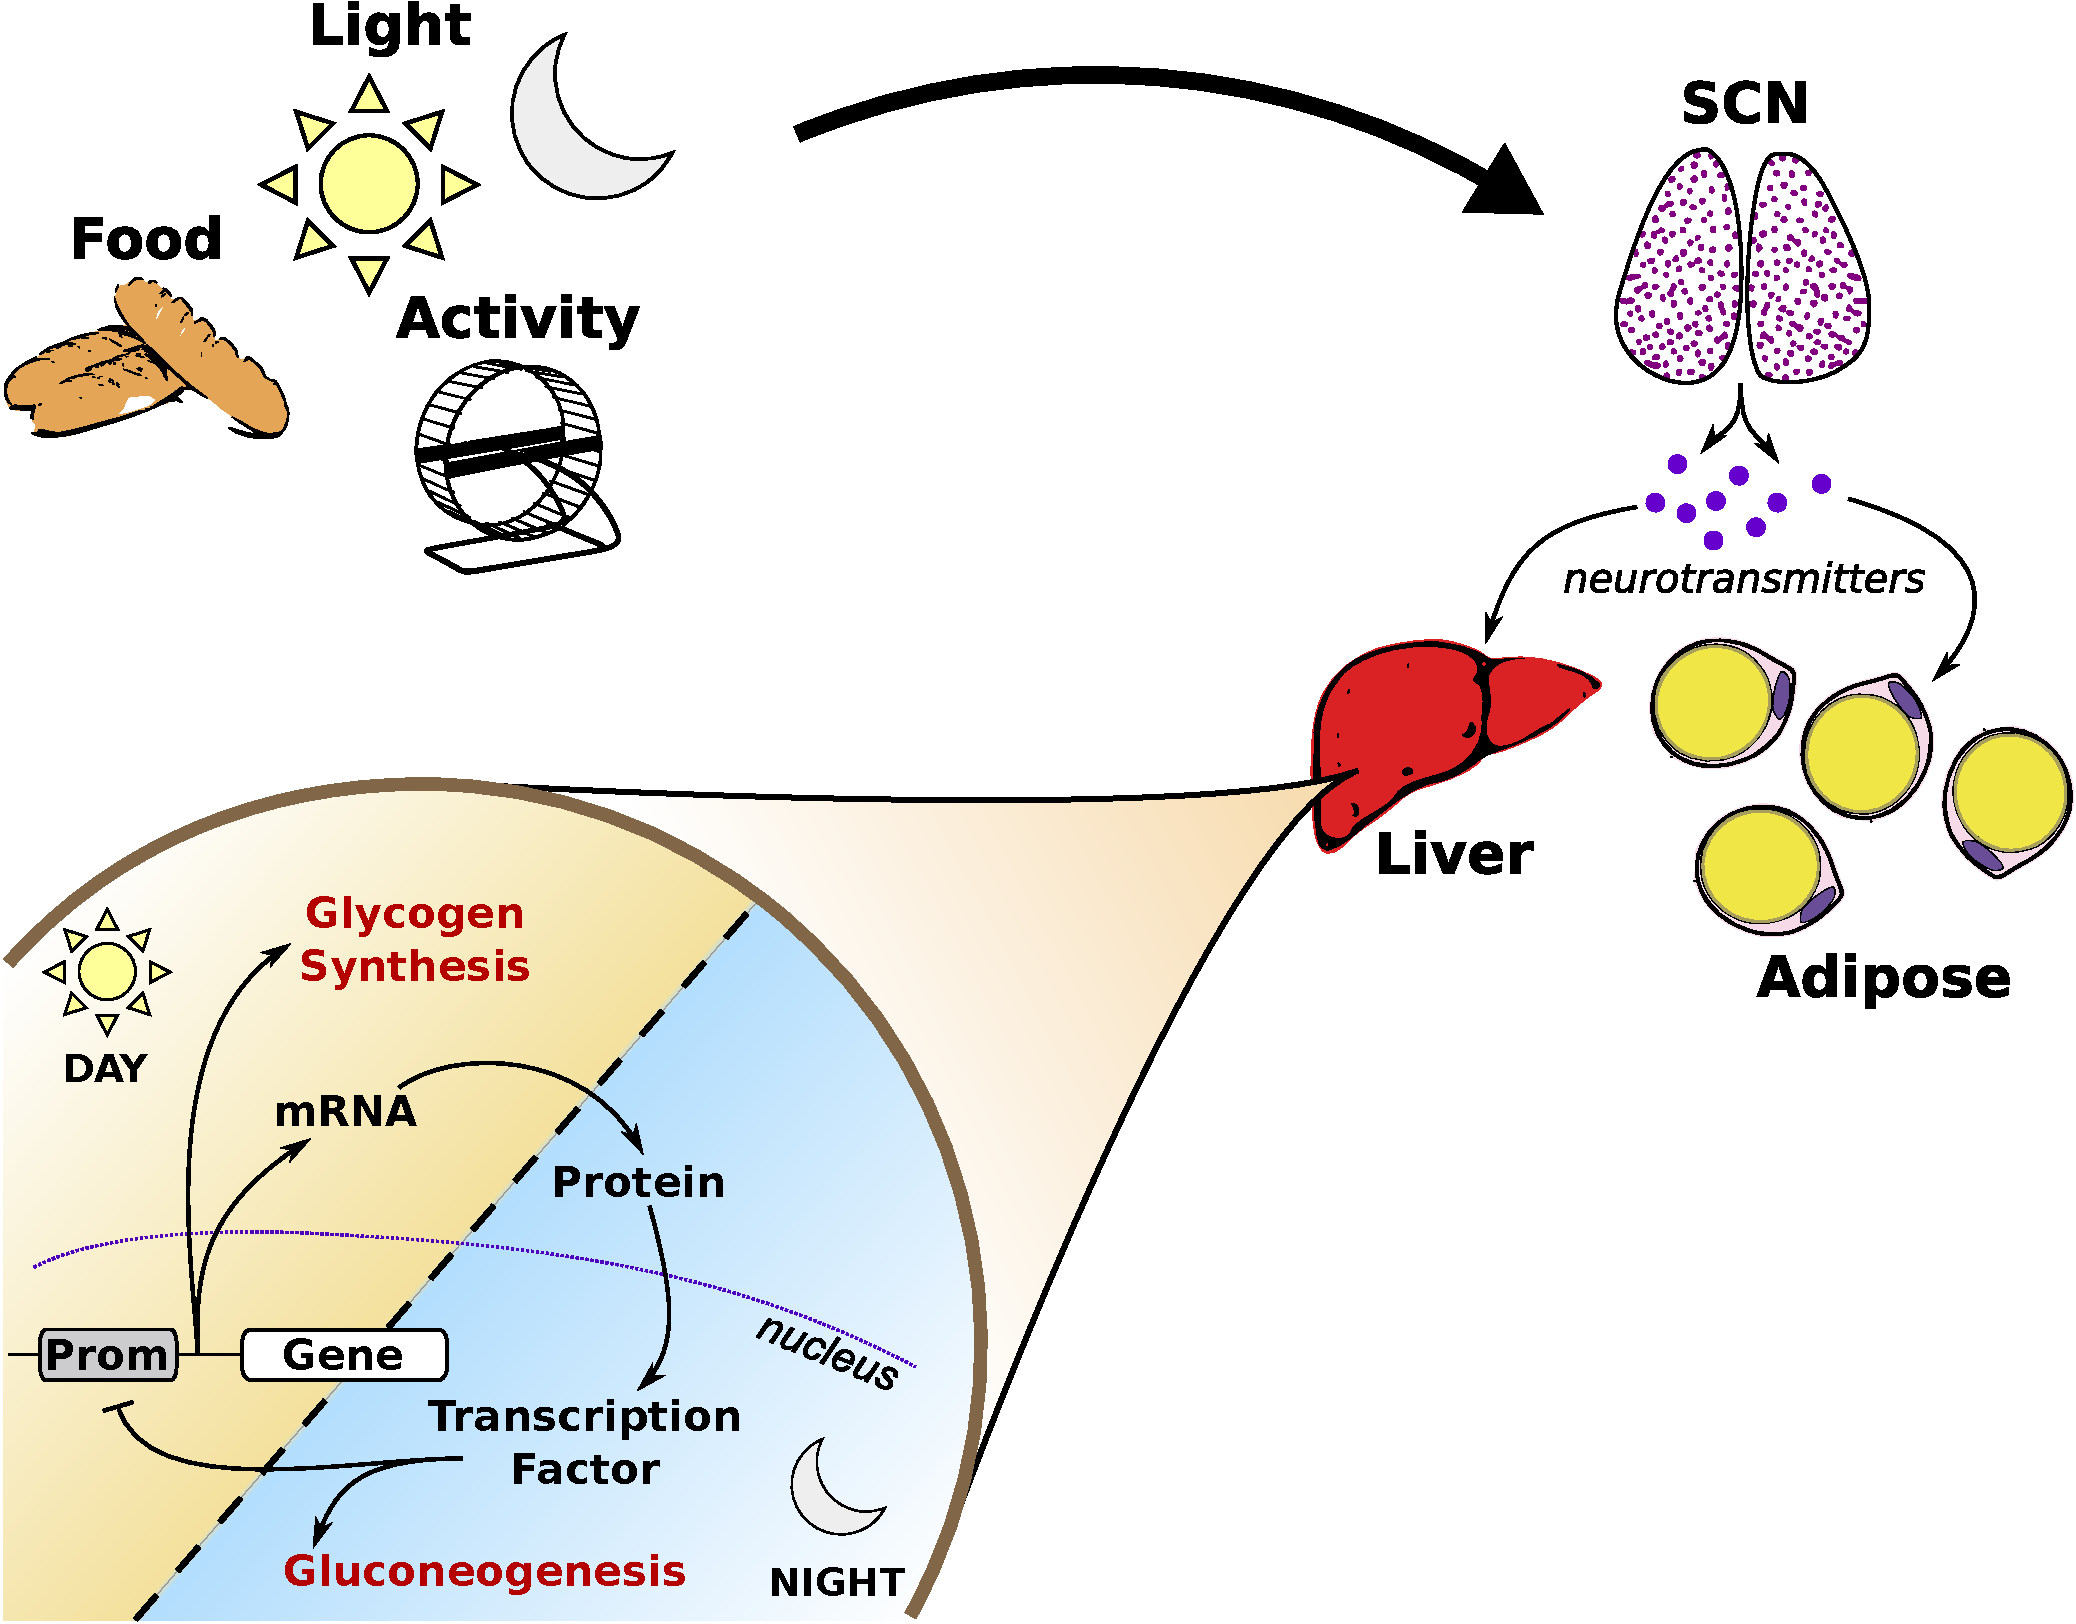
\includegraphics[width=\textwidth]{chap1/figures/timescale_separation.pdf}
  \titlecaption{A biological feed forward controller}{Circadian rhythms are organized in a hierarchical fashion, in which inputs from the environment are processed by different tissue-level clocks. At the single-cell level, rhythms are generated via a time-delayed transcription-translation negative feedback loop. Environmental inputs are used to predict upcoming environmental conditions by speeding or slowing the oscillatory cycle, matching the body's internal phase with the external environment.}
  \label{fig:feedforward}
\end{figure}

Peripheral tissues are responsible for responding to changes daily changes in food intake \cite{Bass2010}. 
Liver and adipose tissue, for instance, maintain robust circadian oscillations \cite{Yoo2004}, which respond mainly to temperature and food resetting cues \cite{Yamazaki2000a}.
Such clocks are important to maintaining metabolic health, as knockout experiments demonstrate that compromised circadian in peripheral tissues leads to many disorders, including diabetes and obesity \cite{Marcheva2010, Shi2013}.
Additionally, feeding cycles have been shown to have a profound impact on  circadian oscillations in peripheral tissues. High-fat or out of phase feeding leads to a reprogramming of oscillatory genes and metabolites 
\cite{Kohsaka2007, Hatori2012}, often leading to metabolic disease.

\subsubsection{Circadian oscillations at the single-cell level}
Circadian rhythms are generated at the single-cell level through genetic regulatory networks with inherent time-delayed negative feedback. 
Transcription factors CLOCK and BMAL1, peaking in the early night, activate expression of EBOX genes period ({\itshape Per1} and {\itshape Per2}) and cryptochrome ({\itshape Cry1} and {\itshape Cry2})\footnote{In this thesis, we denote mRNA species using italics, and protein products using all capital letters.}.
{\itshape Per} and {\itshape Cry} protein products, PER and CRY, peaking during the early day, form a heterodimeric complex to cross the nuclear membrane \cite{Ko2006}. 
However, since PER is present in the cytoplasm in much lower quantities than CRY, it is stochiometrically-limiting for nuclear entry \cite{Lee2001}. 
Once inside the nucleus, the PER-CRY complex dissociates, and CRY represses CLOCK-BMAL1 mediated activation of EBOX genes, leading to rhythmic gene expression.
Several time delays contribute to the 24 hour oscillatory period, highlighted in \fref{fig:maindelays}.

\begin{figure}[tbp]
  \centering
  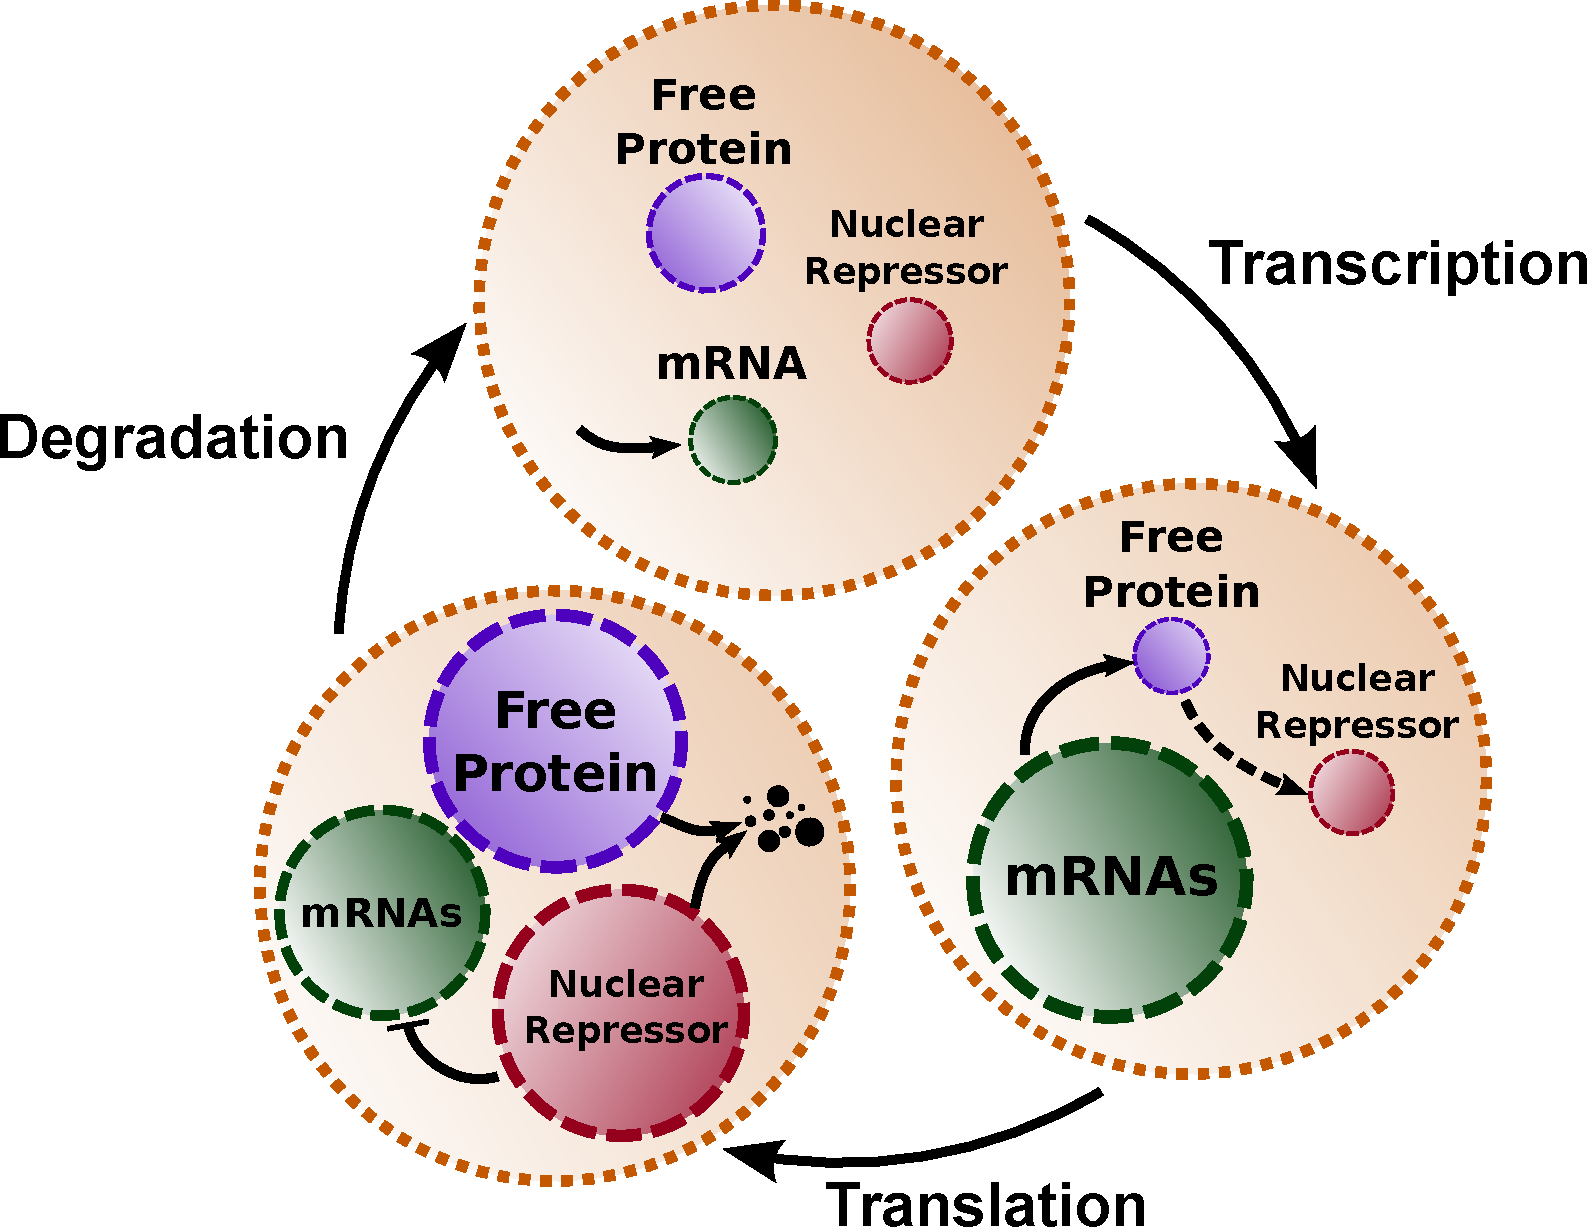
\includegraphics[width=0.7\textwidth]{chap1/figures/maindelays.pdf}
  \titlecaption{Key time delays}{Negative feedback may give rise to sustained oscillations in the presence of time delays. In the circadian system, these time delays are transcription, translation, and protein degradation. Each of these rates is a function of the external environment, resulting in entrainable oscillations.}
  \label{fig:maindelays}
\end{figure}

Additional components, namely the ROR and REV-ERB families of genes, add a layer of positive feedback to the clock regulatory loop.
This addition results in more reliable clock oscillations, as the bistability induced by the positive feedback stabilizes the negative-feedback induced oscillations \cite{Ananthasubramaniam2014a}.
A schematic of the core feedback in mammalian circadian rhythms is shown in \fref{fig:coreloop}.

\begin{figure}[tbp]
  \centering
  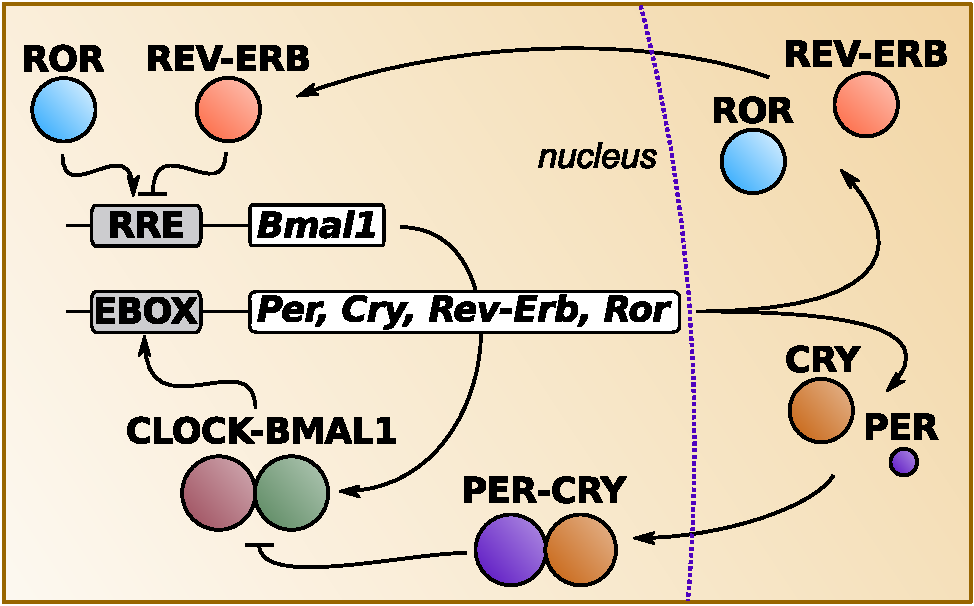
\includegraphics[width=0.7\textwidth]{chap1/figures/coreloop.pdf}
  \titlecaption{Core components of the mammalian circadian feedback loop}{The mammalian feedback loop is comprised of interlocking positive and negative feedback loops.}
  \label{fig:coreloop}
\end{figure}

\subsection{Experimental techniques}

While the focus of this thesis is primarily computational, we present a brief overview of the relevant experimental methods for studying circadian rhythms.
Much of the work presented in this thesis has been performed in collaboration with experimental groups, including Steve Kay's group at the University of Southern California (previously UC San Diego) and Andrew Liu's group at the University of Memphis.

Circadian rhythms are studied in many different types of model organisms, and each organism requires different techniques for studying their behavior.
Some of the earliest work that determined the underlying transcriptional oscillator was performed in {\itshape Drosophila}, where it was shown that mutant fly strains had altered reproduction schedules in constant dark conditions \cite{Panda2002}.
Since many analogs of the genes and proteins responsible for generating circadian rhythms in flies were also present in mammals, including {\itshape Clock, Period,} and {\itshape Cryptochrome}, much of the knowledge gained from studying fly clocks were useful in understanding oscillations in mice \cite{Panda2002}.

Early  experiments determined the roles and importance of mammalian circadian genes using activity data of mouse knockouts in constant darkness \cite{Vitaterna1994}.
For instance, the period-determining effect of CRY1 and CRY2 were found by analyzing wheel-running behavior of mice in plots known as actograms \cite{VanderHorst1999}, as shown in \fref{fig:vanderhorst}.

\begin{figure}[tbp]
  \centering
  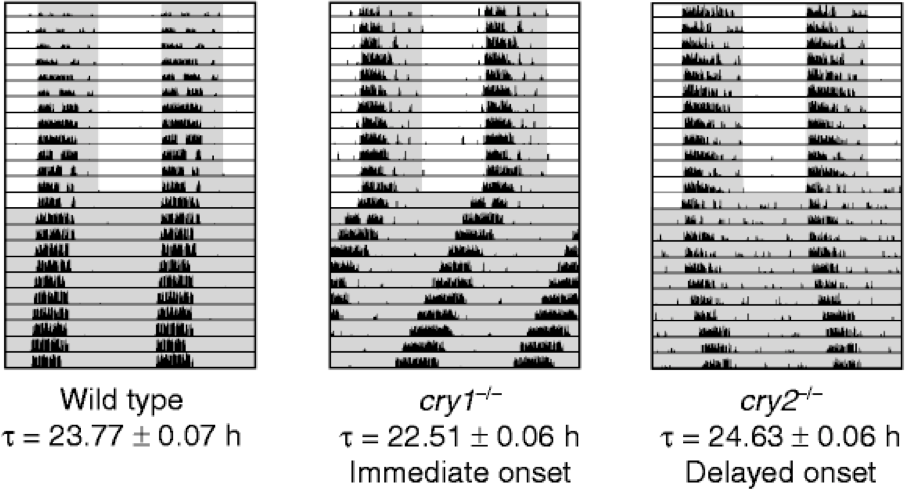
\includegraphics[width=0.7\textwidth]{chap1/figures/vanderhorst.png}
  \titlecaption{Period effects of CRY knockouts}{Actograms plot the intensity of mouse wheel-running activity. The x-axis plots time of day (data is double-plotted), while the y-axis shows each subsequent day. Black bars for each day indicate the intensity of wheel-running activity. After the mice are transferred to constant darkness, the free-running period can be inferred by fitting a line to the offset in activity onset each day. Figure reprinted from \cite{VanderHorst1999}.}
  \label{fig:vanderhorst}
\end{figure}

While activity-level knockout data is still used to characterize the effects of circadian perturbations, such methods are costly to implement and not amenable to high-throughput experimentation.
The development of luciferase reporter cell lines has rapidly changed the way circadian genes are screened \cite{Yoo2004}.
In reporter cells, the coupling of a luciferase protein to a core-clock gene allows the phase of rhythms to be determined by measuring the luminescence output from cultured cells.
Such systems have allowed the development of high-throughput methods for studying how siRNA \cite{Zhang2009} and small molecules \cite{Hirota2008} affect circadian parameters.

As bioluminescence experiments measure the combined output of thousands of individual cells, the synchrony of the population determines in large part the amplitude of the observed rhythms.
While cells in the SCN communicate using intercellular signals to maintain synchrony in rhythms, cultured cells are suspected to lack a mechanism to spontaneously synchronize \cite{Noguchi2013}.
As a result, experiments will determine the rhythmicity of cultured cells by synchronizing the cells at the start of recording and recording the damped oscillations as the cells dephase \cite{Welsh2004}.
While small molecule perturbations are sometimes used, the rhythms of cultured cells are acutely sensitive to their environment, and therefore simply changing the medium is often enough to induce temporary synchrony in oscillations \cite{Izumo2006}.

% \begin{figure}[tbp]
%   \centering
%   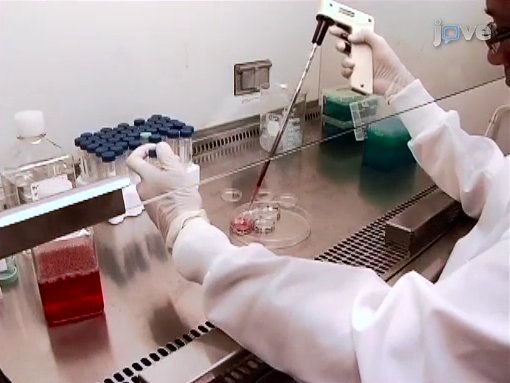
\includegraphics[width=0.45\textwidth]{chap1/figures/cells.png}
%   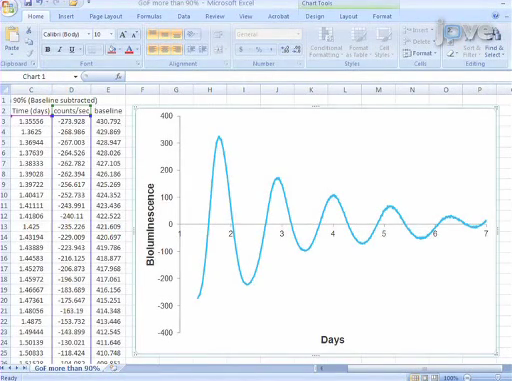
\includegraphics[width=0.45\textwidth]{chap1/figures/data.png}
%   \titlecaption{Monitoring circadian parameters with bioluminescence reporter cell lines}{Cultured reporter cells allow parameters such as amplitude, period, and decay rate to be easily quantified. Image stills from \cite{Ramanathan2012}.}
%   \label{fig:chidalumin}
% \end{figure}

\section{Mathematical modeling}

Circadian rhythms, due to their dynamic nature, have long been the subject of mathematical inquiry \cite{Winfree2001}. In this section, we review some of the methods previously applied to understanding circadian rhythms.
While a wide range of mathematical approaches have been used to model circadian rhythms {\itshape in silico}, here we focus on techniques from ordinary differential equations (ODEs) and stochastic biochemical systems.

\subsection{Introduction to modeling gene regulation}

Gene regulatory networks are typically modeled as dynamic systems, in which rates of production and degradation of each species is explicitly considered.
In \fref{fig:sysbiointro}, an example gene regulatory network is shown, in which a transcription factor activates the production of Gene 1. 
The genes mRNA is then translated to produce a protein product, which may or may not undergo posttranslational modifications or subcellular transport. 
The completed protein then modulates the production of a second mRNA for Gene 2.
In this example, the production and degradation rates of the mRNA and each protein state would be explicitly modeled.

\begin{figure}[tbp]
  \centering
  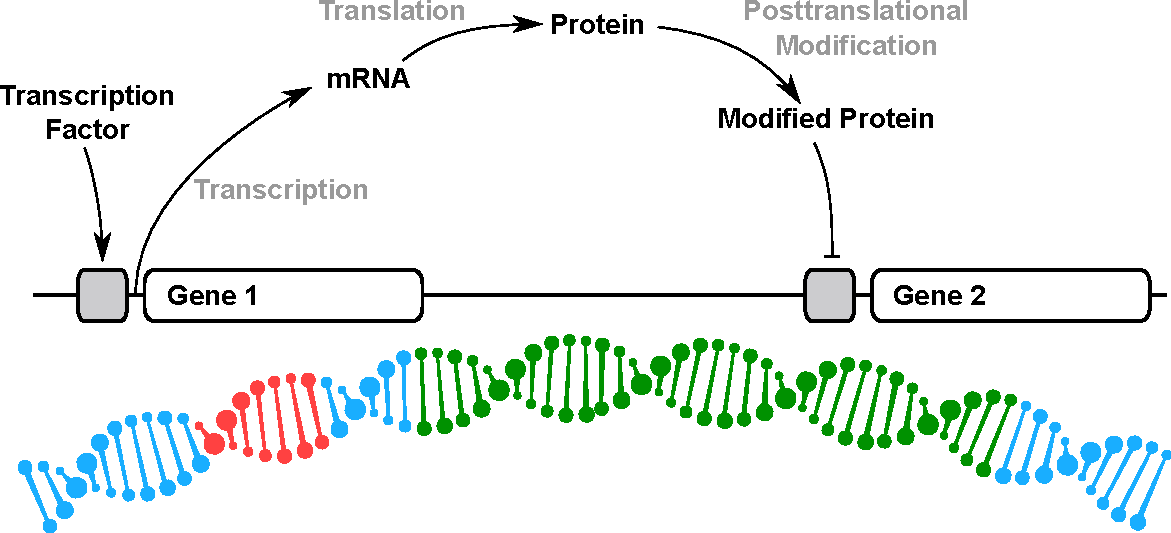
\includegraphics[width=\textwidth, clip=True, trim=0 100 0 0]{chap1/figures/sysbio_intro.pdf}
  \titlecaption{Gene regulatory networks can be modeled as dynamic systems}{Transcription, translation, degradation steps are treated as chemical reactions, in which the reaction rate depends only on the current concentration of other species and various kinetic parameters.}
  \label{fig:sysbiointro}
\end{figure}

If the values of the kinetic parameters (i.e., transcription rate) were known, the model could subsequently be simulated by casting the equations as either a system of ordinary differential equations (as in \fref{sec:odes}), or by using a chemical master equation (as in \fref{sec:stoch}). Resulting trajectories would resemble those shown in \fref{fig:extrajs}.

\begin{figure}[tbp]
  \centering
  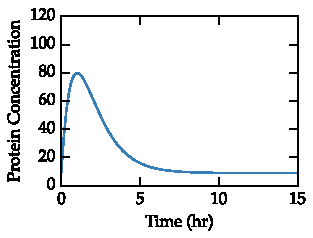
\includegraphics[width=0.475\textwidth]{chap1/figures/sysbio_trajs1.pdf}
  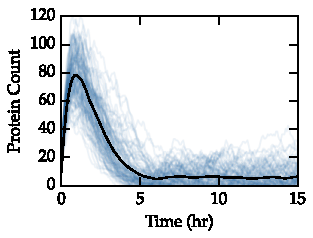
\includegraphics[width=0.475\textwidth]{chap1/figures/sysbio_trajs2.pdf}
  \titlecaption{Simulated time-dependent concentration trajectories}{(Left) Deterministic simulations of the dynamic system result in expected values for each state variable over time. (Right) Stochastic simulations account for the intrinsic noise present due to the low molecule counts of each reactant. From these simulations, more realistic noise estimates can be obtained at the expense of a greater computational complexity.}
  \label{fig:extrajs}
\end{figure}

\subsection{Ordinary differential equations}\label{sec:odes}

Ordinary differential equation (ODE) models take the general form
\begin{equation}
  \frac{dx}{dt} = f(x(t), p),
  \label{eq:odefn}
\end{equation}
in which $x(t)$ represents the concentrations of the state variables, such as mRNA and protein concentrations, $f$ contains information on the production, degradation, and reactivity of the states, and $p$ are the kinetic parameters which govern reaction kinetics.
Limit cycle models are ODE models in which the solution approaches a steady state oscillatory trajectory, satisfying the equation:
\begin{equation}
  \lim_{t \to \infty} \left[ x(t + T) - x(t) \right] = 0.
  \label{eq:limit5}
\end{equation}
The period is the smallest $T > 0$ for which \fref{eq:limit5} holds. 
An example periodic limit cycle is shown in \fref{fig:statespace}, which plots the deterministic solution to \fref{mod:novak}.

\begin{figure}[tbp]
  \centering
  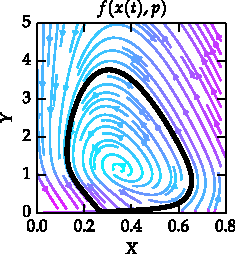
\includegraphics[width=0.45\textwidth]{chap1/figures/state_space.pdf}
  \titlecaption{State-space representation of a deterministic limit cycle}{A two-dimensional oscillator, \fref{mod:novak}, allows the system dynamics to be easily plotted. The steady state limit cycle, $x^\gamma(\theta)$, is shown in dark black. Points which lie off the limit cycle will eventually converge, following the vector field arrows. Colors represent the speed with which the solution will travel, with warmer colors indicating faster speeds.}
  \label{fig:statespace}
\end{figure}


The points on the stable limit cycle are denoted by $x^\gamma(\theta)$ with each point assigned to a value of a phase variable $\theta \in [0, 2\pi)$.
For convenience, time in \fref{eq:odefn} can be rescaled such that the period is $2\pi$:
\begin{equation}
  \tilde{t} = \frac{2\pi}{T}t; \quad \tilde{f} = \frac{T}{2\pi}\;f; \quad \frac{dx}{d\tilde{t}} = \tilde{f}(x(\tilde{t}), p).
  \label{eq:that}
\end{equation}
The phase variable $\theta$ is therefore defined on the limit cycle as $\theta = \tilde{t}\mod 2\pi$, with $\theta = 0$ assigned to a unique and identifiable point. An example mapping of the phase variable $\theta$ for \fref{mod:novak} is shown \fref{fig:phasedef}

\begin{figure}[tbp]
  \centering
  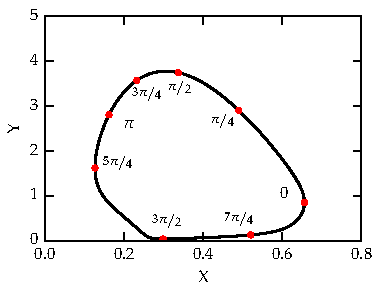
\includegraphics[width=0.5\textwidth]{chap1/figures/phase_def.pdf}
  \titlecaption{Definition of the phase variable}{A phase variable $\theta$ maps each point on the limit cycle, $x^\gamma(t)$, to a unique value of the phase. Because the definition of $\theta$ depends on time, the distance in state-space between each phase point is not equal.}
  \label{fig:phasedef}
\end{figure}


\subsection{ODE sensitivity analysis}

When analyzing ODE models, it is often important to know how the solution varies with respect to initial values or parameters. 
The sensitivity matrix is defined as
\begin{equation}
  S(t) = \frac{dx(t)}{dx(0)} = \lim_{\Delta x(0) \to 0}\frac{\Delta x(t)}{\Delta x(0)}.
  \label{eq:senslimit}
\end{equation}
While it is possible to obtain estimates of these derivatives through finite difference methods, more accurate and less computationally intensive representations can be obtained by integrating these sensitivities along with the original ODE system \cite{Dickinson1976}. 
The differential equation for the sensitivity system is shown in equation~\ref{eq:senslimit}. 
\begin{equation}
  \frac{d}{dt} S(t)  = \frac{df(x(t),p)}{dx}\; S(t)
  \label{eq:odesens}
\end{equation}
Since the jacobian matrix $\frac{\partial f}{\partial y}$ is the same as that of the original ODE system, efficient implementations of the following ODEs have been developed \cite{Feehery1997}.

\subsubsection{Period sensitivity}

An extension of sensitivity analysis for limit-cycle specific models raises additional complications. 
For instance, finding the derivative of the period with respect to parameter values requires a clever decomposition of the sensitivity matrices \cite{Kramer1984}. 
Period sensitivities, $\frac{\partial T}{\partial p}$, can be obtained directly from sensitivities integrated for one pass of the limit cycle (derived in \cite{Wilkins2009}) through a linear solve:
\begin{equation}
  \left[\begin{array}{cc}
      \mathbf{M} - \mathbf{I} & \dot{x}(T) \\
      \frac{\partial f_0}{\partial x}(x(0)) & 0
  \end{array}\right]
  \left[\begin{array}{c}
      \vdots \\ \frac{\partial T}{\partial p}
  \end{array}\right] =
  \left[\begin{array}{c}
      -\mathbf{S}(T) \\ -\frac{\partial {\bm f}}{\partial p}(x(0))
  \end{array}\right]
\end{equation}
in which $\mathbf{M}$ is the Monodromy matrix, $\mathbf{I}$ is the identity matrix, and the unknown vector contains the relevant period sensitivities.

Since parameter values often span several orders of magnitude, an often more useful measure is the relative period sensitivity, which is independent of the magnitude of the period or parameter value.
\begin{equation}
  \frac{\partial \ln T}{\partial \ln p} = \frac{p}{T}\frac{\partial T}{\partial p} = \frac{\partial T}{T} \left/ \frac{\partial p}{p} \right.\label{eq:relperiodsens}
\end{equation}
Thus, a relative period sensitivity of 1 indicates that a 1\% increase in the parameter value will result in a 1\% increase in the period.

\subsubsection{Phase sensitivity}

Perturbations to state variables away from a limit cycle ultimately return, but with in a change of phase.
The definition of phase can be extended to points outside the limit cycle, $x_0 \not\in x^\gamma(\theta)$, by defining the phase of any point, $\Theta(x_0)$, as the initial phase of a point on the limit cycle to which $x_0$ will ultimately converge:
\begin{equation}
  \Theta(x_0) = \arg\min_\theta \lim_{t \to \infty} \lVert x(t)
  - x^\gamma(\theta + t)\rVert
  \label{eq:extendedphase2}
\end{equation}
A phase response curve (PRC), which maps the change in phase resulting from the same
perturbation applied at every phase, can therefore be found by calculating $
\Delta\theta \coloneqq \Theta(x^\gamma(\theta_0) + \Delta x(0)) - \theta_0$ for each
$\theta_0$. Infinitesimal PRCs, the derivative of the phase
change with respect to the perturbation, are defined for state and
parameter-impulse perturbations as \cite{Taylor2008a}:
\begin{align}
  \frac{d\theta}{dx} &\coloneqq \lim_{\Delta x(0) \to 0} \frac{\Delta\theta}{\Delta
  x(0)} \label{eq:sPRC}\\
  \frac{d}{d\hat{t}}\frac{d\theta}{dp} &\coloneqq \lim_{d,\; \Delta p \to 0}
  \frac{\Delta\theta}{d \; \Delta p}
  \label{eq:PRC}
\end{align}
Methods for efficiently calculating these quantities using ODE sensitivity
analysis have been developed \cite{Taylor2008a}, with the important result
that, in the limit as $d, \Delta p \to 0$, 
\begin{equation}
  \frac{d}{d\hat{t}}\frac{d\theta}{dp} = \frac{d\theta}{dx}\frac{d\hat{f}}{dp} 
  \label{eq:pPRCequiv}
\end{equation}

\subsection{Common kinetic assumptions}\label{sec:kinetic}

In constructing an ODE model of a genetic regulatory network, several common kinetic motifs are employed to capture various types of activation, repression, degradation, and complex formation.
In this section, we provide an overview of the kinetic assumptions used for model construction in subsequent chapters.

\subsubsection{Mass action law}

First developed approximately 150 years ago \cite{Voit2015}, the law of mass action is used for all types of chemical systems and forms the basis for subsequent kinetic constructions. 
In mass action kinetics, the reaction rate is proportional to the product of the activities (i.e. concentration) of each reactant.
For example, in the reversible reaction
\[
  A + B \xrightleftharpoons[k_{-1}]{k_{+1}} C,
\]
the reaction rates for the forward and reverse reactions ($r_{+1}$ and $r_{-1}$, respectively) would be
\begin{align*}
  r_{+1} &= k_{+1}[A][B]\\
  r_{-1} &= k_{-1}[C].
\end{align*}
As one molecule of $A$ and $B$ are consumed for each molecule of $C$ produced (and vice-versa for the reverse reaction), the ODE system describing this reaction would be:
\begin{align*}
  \frac{d[A]}{dt} &= k_{-1}[C] - k_{+1}[A][B]\\
  \frac{d[B]}{dt} &= k_{-1}[C] - k_{+1}[A][B]\\
  \frac{d[C]}{dt} &= k_{+1}[A][B] - k_{-1}[C],
\end{align*}
which reaches a fixed point (equilibrium) when $\nicefrac{d[\cdot]}{dt} = 0$, yielding the familiar expression for an equilibrium constant:
\[
  K_{eq} = \frac{k_{+1}}{k_{-1}} = \frac{[C]}{[A][B]}.
\]

\subsubsection{Michaelis-Menten Kinetics}\label{sec:mmenten}

The Michaelis-Menten rate law, first published in 1913 \cite{Johnson2011}, is a commonly used assumption to simplify the kinetics of an enzyme-mediated process.
The full system considered by the Michaelis-Menten model involves the reversible binding of an enzyme to a substrate, and the subsequent irreversible reaction of the enzyme-substrate complex, forming the product:
\begin{equation}
  E + S \xrightleftharpoons[k_r]{k_f} ES \xrightarrow{k_{cat}} E + P.
  \label{eq:mmreactions}
\end{equation}
The full ODE system for \fref{eq:mmreactions} is therefore
\begin{align}
  \frac{d[S]}{dt} &=  -k_f[E][S] \label{eq:S}\\
  \frac{d[E]}{dt} &= k_{cat}[ES] + k_r[ES] - k_f[E][S] \label{eq:E}\\
  \frac{d[ES]}{dt} &= k_f[E][S] - k_r[ES] - k_{cat}[ES] \label{eq:ES}\\
  \frac{d[P]}{dt} &= k_{cat}[ES]. \label{eq:P}
\end{align}
Since the concentration of enzyme-substrate complex, $[ES]$ is often difficult to measure experimentally, the above system of equations is typically not applied to real data.
Instead, a pseudo-steady state assumption (PSSA) is made, in which the equilibrium $E + S \xrightleftharpoons[k_r]{k_f} ES$ is assumed to equilibrate much faster than the product formation, $ES \xrightarrow{k_{cat}} E + P$.
This assumption results in $\nicefrac{d[ES]}{dt} \approx 0$, which can be used to simplify the above set of equations. 
We also assume a conservation of enzyme mass, $[E_T] = [E] + [ES]$. 
By solving the now-algebraic equations \ref{eq:E}-\ref{eq:ES} for $[E]$ and $[ES]$ and substituting the resulting expression into the remaining equations, we obtain:
\[
  [ES] = \frac{[E_T][S]}{\nicefrac{k_r}{k_f} + [S]}
\]
from which the production rate of the product is determined:
\begin{align*}
  \frac{d[P]}{dt} = \frac{V_{max}[S]}{K_M + [S]}, & & V_{max} = k_{cat}E_T, & \quad K_M = \frac{k_r}{k_f}.
\end{align*}
While the Michaelis-Menten model is widely used for enzyme-catalyzed reactions in biology, some articles have argued that the assumptions are likely not valid for protein-protein interactions, in which the substrate and enzyme are present in comparable concentrations \cite{Tzafriri2004}.

\subsubsection{Enzyme inhibition}
The Michaelis-Menten kinetic assumption can be extended to model the effects of enzyme inhibitors.
Different types of enzyme inhibition are possible, in which an inhibitor $I$ binds to the free enzyme $E$ and/or the enzyme-substrate complex.
In competitive inhibition, the inhibitor binds only to the free enzyme complex, blocking the binding of the substrate.
\begin{equation}
  E + I \xrightleftharpoons[k_{-i}]{k_{i}} EI
  \label{eq:compinh}
\end{equation}
Adding \fref{eq:compinh} to \fref{eq:mmreactions} and invoking the PSSA once more, we find the final rate for the conversion of substrate to product:
\begin{align}
  \frac{d[P]}{dt} = \frac{V_{max}[S]}{K_M\left(1 + \frac{[I]}{K_I}\right) + [S]}; & & K_I = \frac{k_{-i}}{k_i}.\label{eq:inheq}
\end{align}

\subsubsection{Hill-type kinetics}

In biochemical systems, cooperative binding between species is often required to initiate a reaction. 
The kinetics of such systems follow a sigmoidal profile, in which a critical amount of reactant species is required before significant product formation is seen, but which quickly saturates to a maximum value. 
The equation describing cooperative binding behavior was developed in 1910 \cite{Hill1910}. Assuming the conversion of reactant $S$ to product $P$, the rate of production of $P$ would follow
\begin{equation}
  \frac{d[P]}{dt} = \frac{V_{max} [S]^n}{K_A^n + [S]^n}
  \label{eq:hill}
\end{equation}
Depending on the degree of cooperativity $n$, the sigmoidal profile can vary between a standard Michaelis-Menten profile (no cooperativity) to an almost digital switch, as shown in \fref{fig:hillshapes}.
Hill-type kinetics can also include enzyme inhibition, in which the $K_A$ parameter would be scaled by inhibitor concentration in a manner similar to \fref{eq:inheq}.

\begin{figure}[tbp]
  \begin{center}
    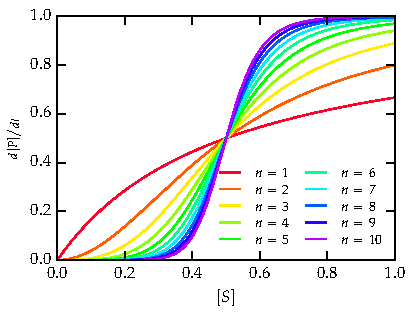
\includegraphics[width=0.6\textwidth]{chap1/figures/hilleq.pdf}
  \end{center}
  \titlecaption{Example profiles of the hill equation for various degrees of cooperativity}{The hill equation describes the kinetics of a cooperative reaction process, as shown in \fref{eq:hill}. Here $K_A = 0.5$, $V_{max} = 1$.}
  \label{fig:hillshapes}
\end{figure}


\subsection{Stochastic methods}\label{sec:stoch}

In modeling a system of chemical reactions using ODE methods, the assumption is made that the concentration of reacting species can take any continuous value. 
While this assumption is often appropriate for reactions in large, well-mixed vessels, it is often not the case in reactions that take place in the cell.
In mammalian cells, the median number of mRNA transcripts per cell is $17$, while the median number of protein copies is $50,000$ \cite{Schwanhausser2011}.
As a result, low concentrations of state variables are often best represented by discrete steps, in which the probabilistic nature of reaction events plays a large role in determining the system dynamics.

Stochastic systems are specified by a state vector of discrete populations $x = \{x_1, \ldots, x_N\}$ and reaction vector $R = \{R_1, \ldots, R_M\}$. 
For each of $M$ reactions, a stoichiometric vector $v_i$ describes the states which are produced and consumed by each reaction, and a reaction propensity function $a_i$ describes the likelihood of the reaction in for time step \cite{Gillespie1977}.
Together, these equations form the chemical master equation, a Markov (memoryless) process which can be efficiently simulated using a variety of algorithms \cite{Sanft2011}.


\subsection{Parameter estimation}

Models are typically used to validate that our assumed mechanisms are mathematically feasible, and to systematically explore consequences of our kinetic assumptions.
When these models differ from experimental results, we must re-analyze which of our assumptions might be incorrect and design new experiments to test these assumptions.
While biological insight is typically sufficient to construct candidate models $f(x, p)$ using standard assumptions outlined in \fref{sec:kinetic}, values for the kinetic parameters are typically derived by fitting experimental data.
In this section, we describe optimization techniques which have proven successful in finding descriptive parameter sets for models of circadian rhythms.

\subsubsection{Cost function}

The first step in finding a suitable parameter set is defining a cost function, $C(p)$, which ascribes a value to how well a particular parameter set fits the data.
By convention, the optimum parameter set is that which minimizes $C(p)$.
While for many biological systems a suitable cost function is the squared error of the model, a cost function can also include information on model derivatives, oscillatory period, and timing of various events (i.e., peak gene expression).
Cost functions of limit cycle models pose a particularly difficult optimization challenge, as a limit cycle does not always exist for any given parameter set.
Thus, the fitness landscape for most parameter space is very flat where limit cycle solutions do not exist, with isolated regions of  where limit cycle oscillations are possible.
Additionally, solving for the limit cycle solution given a parameter set is a nested optimization problem, resulting in long computation times.
For these reasons, stochastic global optimization procedures are often employed which efficiently search high dimensional parameter space without the need for derivative information of $C(p)$.
An overview of the computational approach typically employed for such systems is given in \fref{fig:comploop}.

\begin{figure}[tbp]
  \centering
  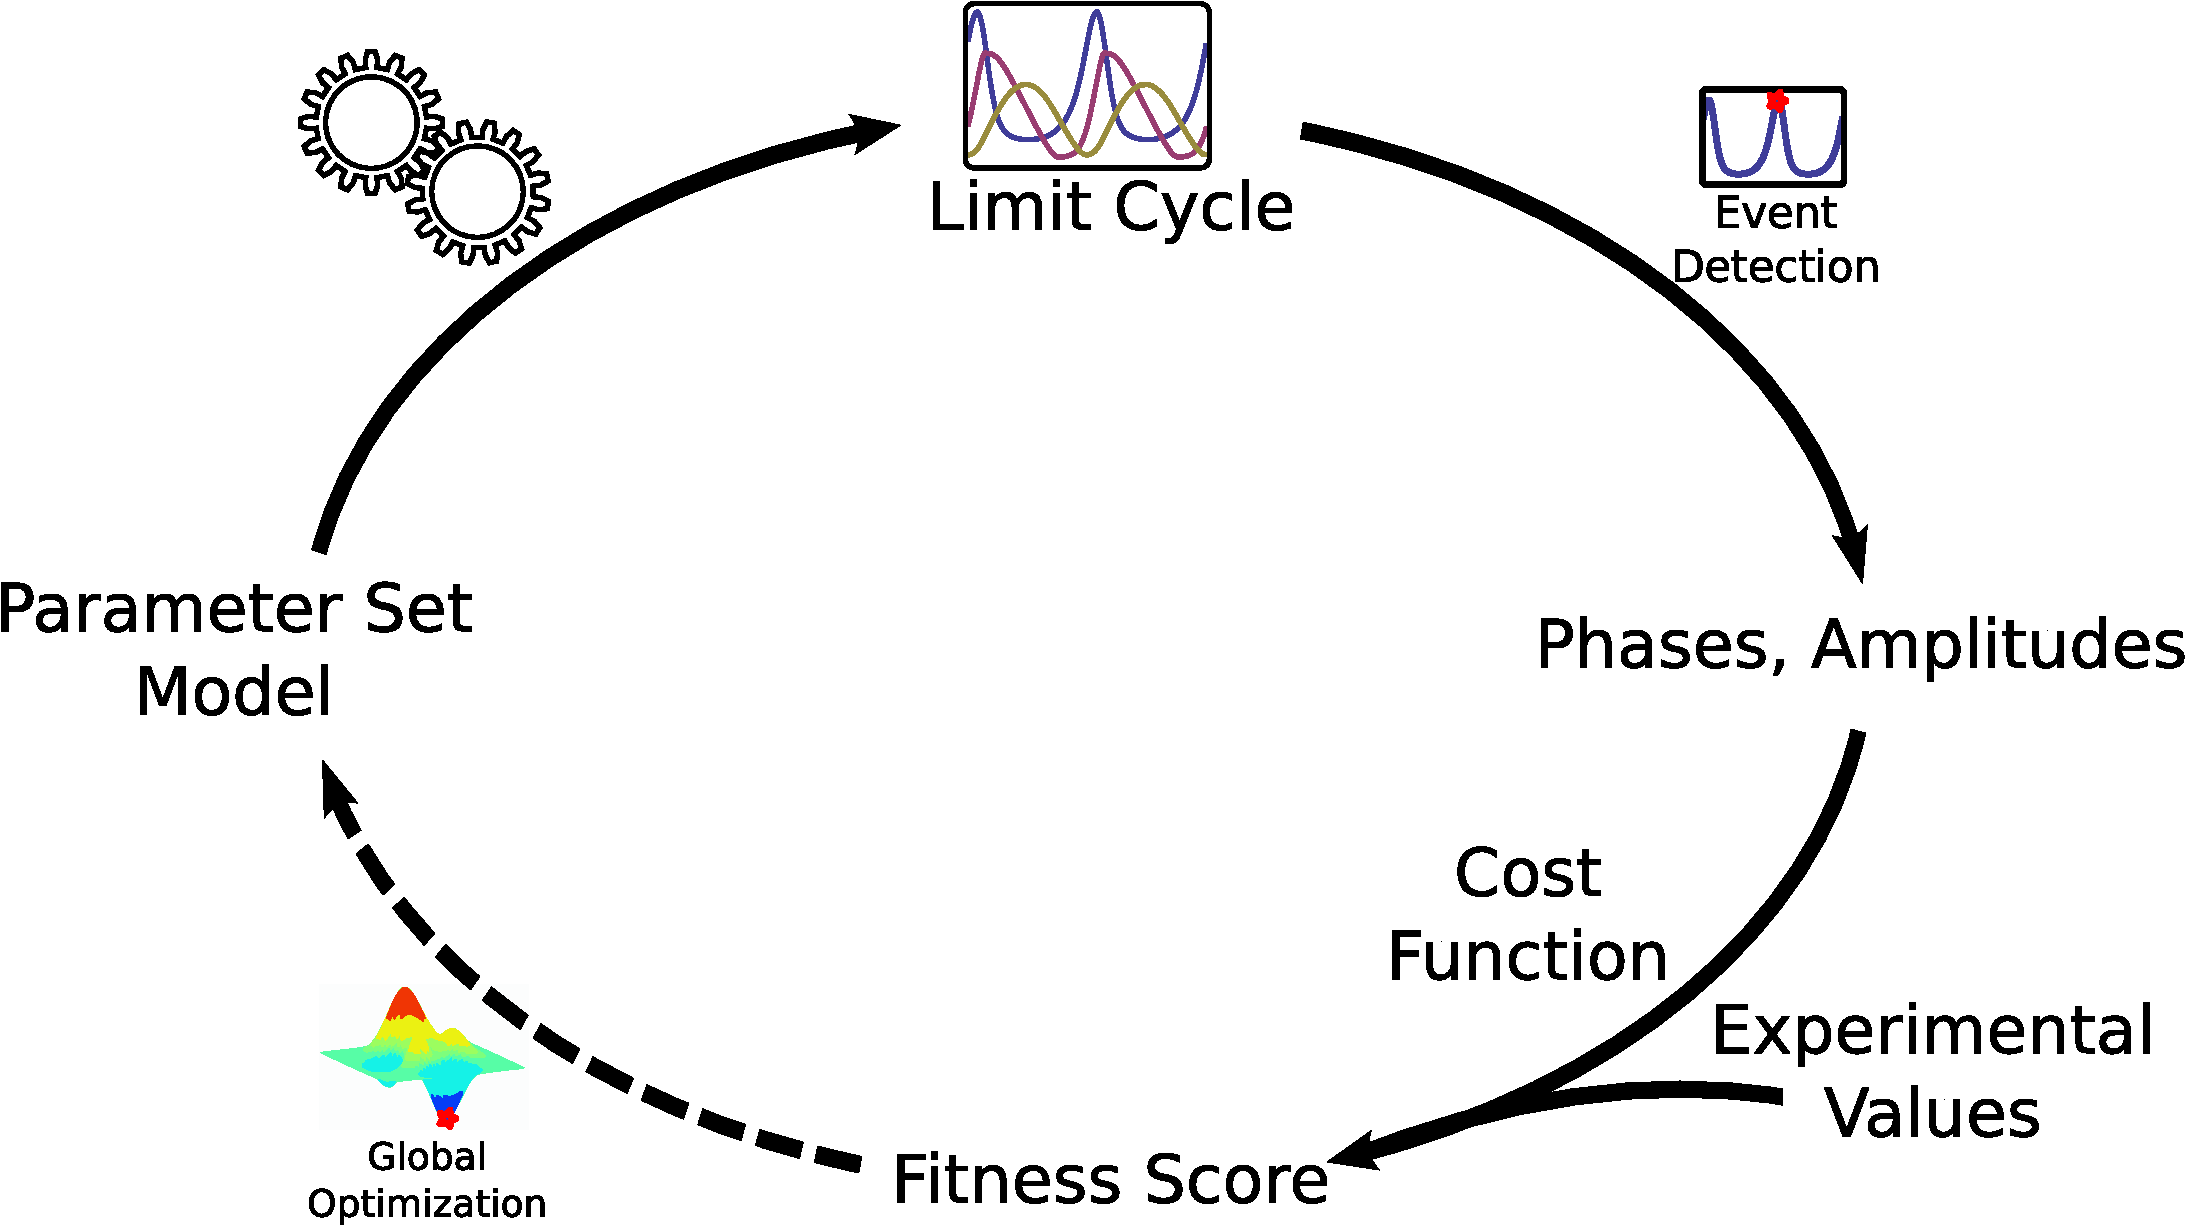
\includegraphics[width=0.65\textwidth]{chap1/figures/comp_loop.pdf}
  \titlecaption{An overview of the nested optimization of fitting limit cycle models}{Given a model and parameter set guess, a limit cycle is calculated via a single-shooting approach. A cost function then scores the timing of peak mRNA and protein species against known experimental values. Given the fitness score of many parameter guesses, a global optimization algorithm iteratively improves the parameter guess to minimize the cost function.}
  \label{fig:comploop}
\end{figure}

\subsubsection{Global optimization}\label{sec:gas}
In this thesis, global optimization of model parameters is typically achieved via an evolutionary algorithm approach \cite{Whitley2001}. 
An evolutionary algorithm iteratively improves a parameter guess in an easily-parallelized fashion by mimicking natural evolution.
The steps involved are as follows, shown schematically in \fref{fig:gaoverview}.
\begin{enumerate}
  \item {\bfseries Initialization} An initial population of parameter guesses are generated from all parameter values, typically by a random number generation.
  \item {\bfseries Selection} The fitnesses (inverse of the cost) of the current population are evaluated, and a subsample of the original population is selected. A selection algorithm must randomly select from the current population, with some degree bias given towards individuals with the highest fitness.
  \item {\bfseries Crossover} Each member of the subsequent generation of solutions is generated by combining features from two (or more) of the selected individuals in the previous generation. For a problem consisting of many individual parameters, a common choice is to randomly select each parameter from one parent or the other.
  \item {\bfseries Mutation} The final step involves adding a small chance to change a parameter in the child parameter set. For continuous parameter values, this is often implemented as a small chance to add normally-distrusted error to one or more of the parameter values.
\end{enumerate}

\begin{figure}[tbp]
  \centering
  \begin{tabular}{cccc}
    \bf Initialization & \bf Selection & \bf Crossover & \bf Mutation \\
    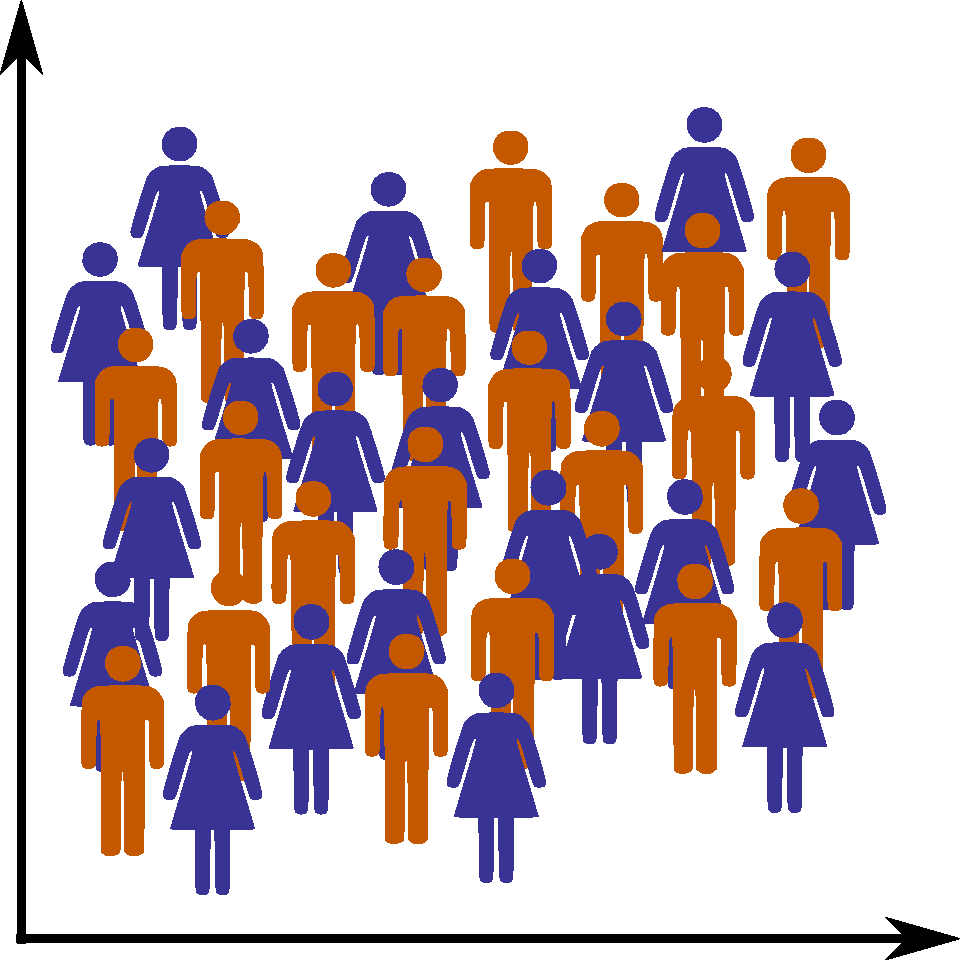
\includegraphics[width=0.2\textwidth]{chap1/figures/ga_initialization.pdf} &
    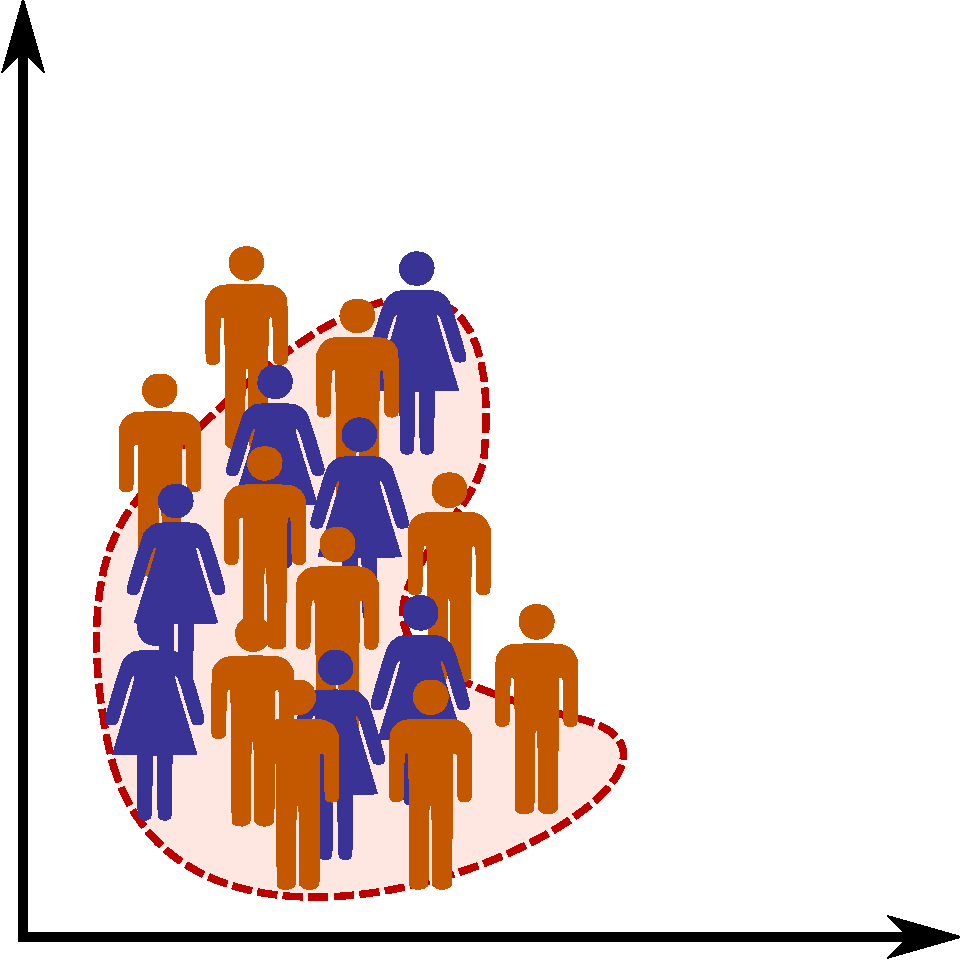
\includegraphics[width=0.2\textwidth]{chap1/figures/ga_selection.pdf} &
    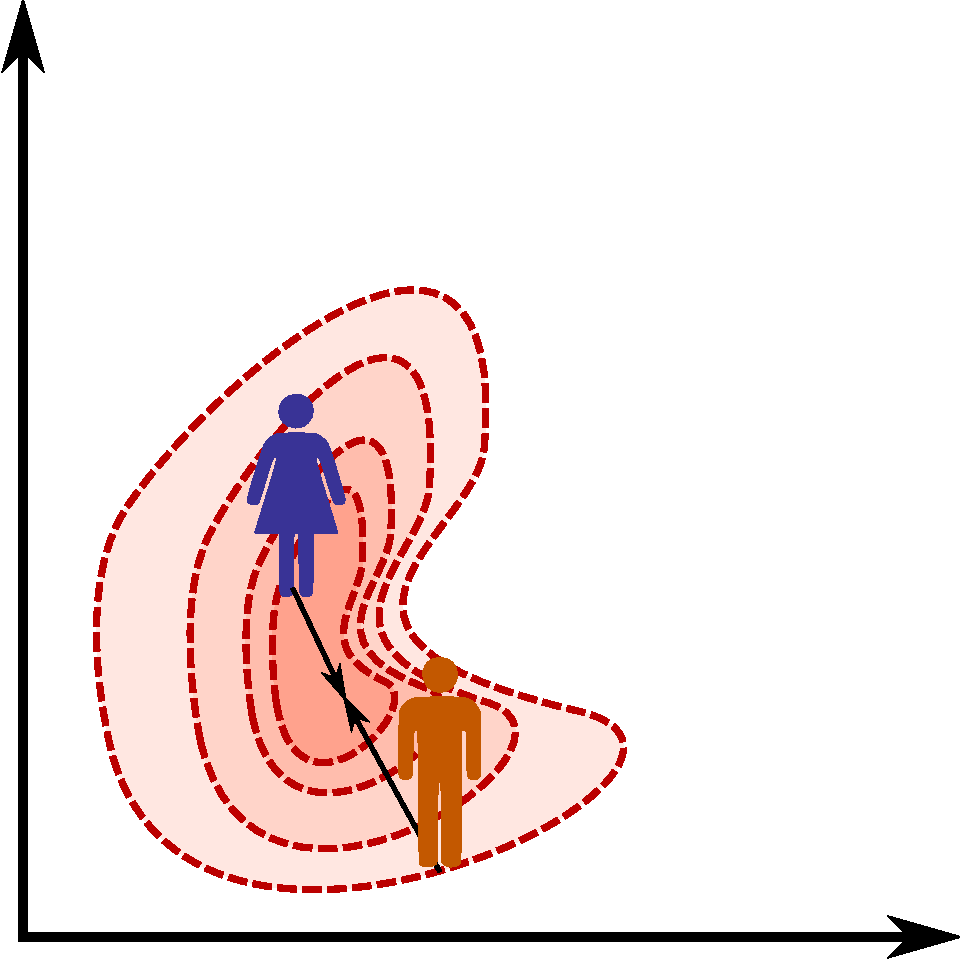
\includegraphics[width=0.2\textwidth]{chap1/figures/ga_crossover.pdf} &
    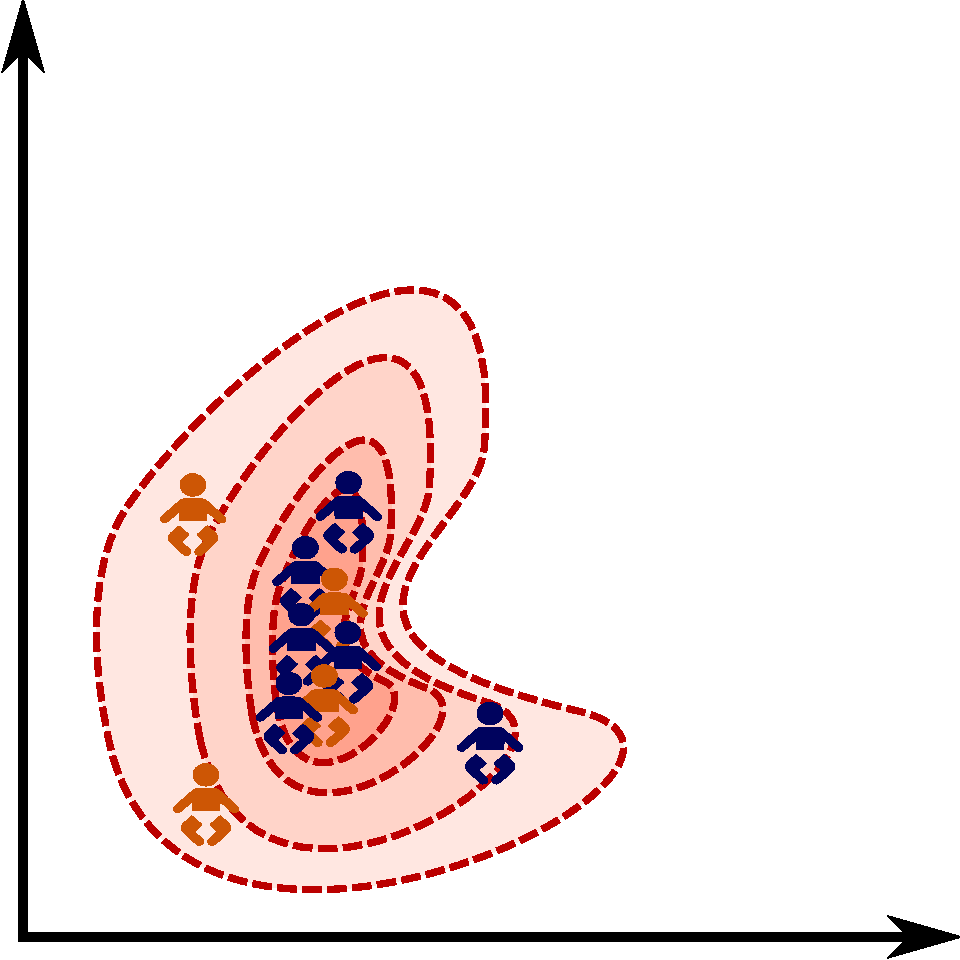
\includegraphics[width=0.2\textwidth]{chap1/figures/ga_mutation.pdf}\\
  \end{tabular}
  \titlecaption{An overview of global optimization via evolutionary strategy}{A schematic of a two-dimensional parameter space is shown. Solutions are initially distributed randomly across the parameter landscape, but solutions with a high fitness are preferentially kept. By combining and slightly altering parameter values from existing solutions, each generation iteratively approaches the highest fitness.}
  \label{fig:gaoverview}
\end{figure}

\subsection{Previous models of circadian rhythms}

Since mathematical methods have been used to study circadian rhythms for some time, many existing models of circadian gene regulation exist.
A summary of the models discussed in this section is presented in \fref{tab:models}.
Early examples include Goodwin's 1965 model of enzymatic oscillations, demonstrating that nonlinear oscillations could capture many of the features of biological rhythms \cite{Goodwin1965}. 
Later models sought to describe specific proteins in the circadian cycle. 
Goldbeter's 1995 model described one gene in the circadian clock of {\it Drosophila}, and demonstrated that a negative feedback loop with sufficient nonlinearity and time delay was required for circadian oscillations \cite{Goldbeter1995}.

\begin{table}[tbp]
  \centering
\begin{tabular}{rrrrc}\toprule
First Author & Year & States & Parameters & Citation             \\\midrule
Goodwin      & 1965 & 2      & 5          & \cite{Goodwin1965}   \\
Goldbeter    & 1995 & 5      & 15         & \cite{Goldbeter1995} \\
Leloup       & 2003 & 16     & 52         & \cite{Leloup2003}    \\
Forger       & 2003 & 73     & 38         & \cite{Forger2003}    \\
Mirsky       & 2009 & 21     & 132        & \cite{Mirsky2009}    \\
Kim          & 2012 & 180    & 70         & \cite{Kim2012}       \\\bottomrule
\end{tabular}
\titlecaption{Summary of ODE models for the circadian network}{While Goodwin's model considers an arbitrary oscillatory biochemical system, it has been frequently invoked to model circadian oscillations in a simple framework.}
\label{tab:models}
\end{table}


Subsequent models have attempted to generate a more complete representation of the circadian network. 
Leloup and Goldbeter's 2003 model of the mammalian circadian clock considers both the positive and negative regulatory loops \cite{Leloup2003}, demonstrating the anti-phase oscillations of the positive and negative elements. 
Forger and Peskin's 73-state model, and its analogous stochastic version, provides an example of the complexity of the known post-translational regulation of core clock components \cite{Forger2003,Forger2005}.

More recently, models have focused on explaining new theories on how circadian rhythms are organized, rather than attempting to providing a complete {\itshape in silico} representation of current knowledge.
A model by To {\itshape et al.,} 2007 coupled together cells modeled by Leloup \& Goldbeter's 2003 model to demonstrate how heterogeneous populations of oscillators could synchronize in an SCN environment using the neurotransmitter vasoactive intestinal polypeptide (VIP) \cite{To2007}.
Following the differentiation between the properties of single-cell oscillators and populations, Mirsky {\itshape et al.,}, 2009 developed a model to show how single-cell knockout phenotypes could be differentiated from those at the population-level \cite{Mirsky2009}.
Rel{\'o}gio {\itshape et al.,} 2011 demonstrated that positive feedback through ROR/REV-ERB had a stabilizing effect on the clock \cite{Relogio2011}, while a model from Kim \& Forger, 2012 demonstrated the importance of stoichiometry between positive and negative components \cite{Kim2012}.
However, despite the wide availability of mathematical models for circadian rhythms, demonstrating that new theories are mathematically rigorous often requires the creation of a new model.

\section*{Thesis Overview}
In \fref{chap:model}, a new model of the core circadian feedback loop is developed in order to explain experimental observations on the effect of a new small molecule modulator.
This new model enables new insights into the functional roles of the two isoforms of mammalian Cryptochrome, CRY1 and CRY2.
In \fref{chap:id}, a method of fitting oscillatory models is presented which uses nonlinear programming rather than the more computationally intensive global optimization strategies typically employed with circadian models.
Using such a method, a bootstrap approach is possible which allows the quantification of confidence intervals in the predicted responses generated from the models.
This method is then applied to a set of three circadian models in \fref{chap:longdaysin} to explain the separate amplitude effects of two small molecule regulators by finding predictions which are consistent across slight differences in kinetic assumptions and parameter value.
In \fref{chap:arc}, we derive a new type of sensitivity analysis for oscillatory models that we denote the amplitude response curve (ARC).
The ARC allows the effect from a temporary pulse, coming perhaps from a small molecule therapeutic, on amplitude to be calculated.
This method allows the systematic investigation of factors which change clock amplitude to proceed efficiently, without the need for more expensive stochastic simulations of a population of oscillators.
Finally, in \fref{chap:decay}, it is shown that damping rate of cultured circadian reporter cells can be a reliable indicator of single-cell noise.
Using this insight, we analyze data from high-throughput siRNA screens to determine the effects of genome-wide gene knockdowns on the stochastic noise.
From this analysis we conclude that the unperturbed clock is highly optimized for robustness, as it lies near the pareto front of high amplitude and low stochastic noise.



\chapter[Modeling the core circadian feedback loop to determine the effect of KL001]{Modeling the core circadian feedback loop to determine the effect of KL001\footnote{ Portions of this chapter are published in T. Hirota, J. W. Lee, P. C. St. John, M. Sawa, K. Iwaisako, T. Noguchi, P. Y. Pongsawakul, T. Sonntag, D. K. Welsh, D. A. Brenner, F. J. Doyle, P. G. Schultz, and S. A. Kay, ``Identification of Small Molecule Activators of Cryptochrome.,'' {\itshape Science}, vol. 337, pp. 1094–1097, July 2012.}}\label{chap:model}

\section{Background}

\subsection{Small molecule modulators}
Circadian rhythms help to regulate metabolic homeostasis, and therefore compromised circadian oscillations often result in negative health consequences.
Since circadian rhythms may be damped by lifestyle factors, many researchers have begun searching for pharmacological agents which might alter circadian rhythmicity.
Several proof-of-concept molecules have been found which cause dose-dependent period change in cultured fibroblasts \cite{Chen2013}.
While chemical biology approaches are able to localize the effects of these molecules to specific targets in the circadian network, it is often difficult to reconcile individual rate changes with the observed systems-level changes in period or amplitude.
Mathematical models are therefore essential to understanding the effects of such drugs, as they are able to verify that hypothesized mechanisms of action are mathematically consistent.
Furthermore, mathematical models provide a systematic framework by which to examine consequences of various mechanistic assumptions - many of which can be subsequently verified by experimental inquiry.
The search for small molecule modulators of circadian rhythms therefore yields the added benefit of strengthening our knowledge of the core clock feedback circuit, as inconsistencies between assumed kinetics and experimental results often lead to a more refined knowledge of the network's dynamics.

In this chapter, I describe a collaborative project in which experimental results inspired the creation of a new model of the core mammalian feedback network.
A new small molecule modulator of cryptochrome, KL001, was identified through forward chemical genetic screening \cite{Hirota2012}.
The compound was found to simultaneously increase the half-life of CRY and cause period lengthening.
In order to explain these new experimental results while maintaining consistency with published evidence, I constructed a simple mathematical model of the PER/CRY negative feedback loop.

The functional roles of the cryptochrome isoforms ({\it Cry1} and {\it Cry2}) in circadian rhythms have long eluded biologists, as although they share a similar structure, perturbations to these genes typically result in opposite trends \cite{McCarthy2009}.
Existing genetic evidence and siRNA knockdown studies agree that while suppressing {\it Cry1} leads to shorter periods, suppressing {\it Cry2} leads to longer periods \cite{VanderHorst1999, Zhang2009}.
However, some evidence shows the similarity between the two {\it Crys}.
The knockouts\footnote{Wild type mammals, denoted with the ``$+/+$'' superscript, receive two copies of every gene from each parent. Homozygous knockouts, denoted ``$-/-$'', have no functional copies of the gene. Heterozygous knockouts, denoted ``$+/-$'', receive only one functional copy and therefore express the gene at lower levels.} $\text{\it Cry1}^{+/-}$ $\text{\it Cry2}^{-/-}$ and $\text{\it Cry1}^{-/-}$ $\text{\it Cry2}^{+/-}$ both show shorter wheel-running activity their respective WT/double knockouts $\text{\it Cry1}^{+/+}$ $\text{\it Cry2}^{-/-}$ and $\text{\it Cry1}^{-/-}$ $\text{\it Cry2}^{+/+}$ \cite{VanderHorst1999}.
Using new data from the application of KL001 together with existing experimental results, I developed a hypothesized mechanism to reconcile these seemingly contradictory results:

\subsubsection{Network structure}
In the core feedback loop, {\itshape Per} and {\itshape Cry} transcription is activated by the CLOCK-BMAL1 complex.
The protein products of these genes are transported to the nucleus after a time delay and bind to CLOCK-BMAL1, repressing their own transcription.
Evidence indicates that an interaction of PER and CRY proteins is required for the timely nuclear entry of both proteins \cite{Miyazaki2001,Ko2006,Kume1999}.
I therefore assume that PER and CRY bind and enter the nucleus in a 1:1 stoichiometric ratio, similar to more complicated models of mammalian circadian rhythms \cite{Leloup2003,Mirsky2009,Forger2003}.

\subsubsection{Protein stoichiometry}
Quantitative protein assays have revealed that the PER proteins are present at levels nearly ten times less than the CRYs, and are completely consumed at their trough.
The CRYs, on the other hand, only fall to about one quarter of their peak value  \cite{Lee2001}.
These results indicate that PER is the rate-limiting component for nuclear entry.
This configuration explains why, since {\itshape Cry} is in excess, a knockout of either {\it Cry} alone does not lead to loss of function at the tissue level.
Additionally CRY1, the more dominant repressor, is consistently found at higher levels than CRY2.
However, since the ratio of nuclear to total protein is nearly equivalent for CRY1 and CRY2, PER must import each with equal affinity \cite{Lee2001,Lee2011b}.

\subsubsection{Importance of degradation}
Studies of the simplest cellular oscillators have illustrated the importance of the degradation of repressor complexes in determining the period of oscillation \cite{Cookson2009}.
In the mammalian circadian clock, FBXL3 has been indicated as a key protein in clearing the nucleus of CRY, and siRNA knockdowns of {\it Fbxl3} result in period lengthening \cite{Zhang2009}.
While FBXL3 localizes primarily in the nucleus, CRY2 possesses a distinct phosphorylation domain that flags it for cytosolic proteolysis \cite{Kurabayashi2010}.
Knocking down this domain shortens the period, indicating that degradation rates play a major role in determining the oscillatory period and that stabilization in the cytosol and nucleus are likely not equivalent.

\subsubsection{Key time delays}
Similar to {\it Drosophila}, mammalian circadian oscillations are generated by three main time delays in the negative feedback loop: mRNA transcription, nuclear localization of protein, and degradation of the nuclear complexes \cite{Vielhaber2000a}.
In order to capture these dynamics without introducing unnecessary stiffness, I explicitly consider only the concentrations of nuclear mRNA, cytosolic unbound protein, and nuclear protein complexes.

\section{Results}

\subsection{A new model for period regulation}
Since the circadian clock is largely insensitive to the total amount {\it Cry}, it follows that the core negative loop is comprised of two redundant coupled inhibitory mechanisms. 
The natural periods of these two loops (running in isolation of the other) can be inferred from their corresponding knockout phenotype, i.e., the CRY1 feedback loop has a long period, while the CRY2 loop has a short period. 
In the wild-type phenotype, the two isoforms of CRY must compete for the available PER, and thus the nuclear CRY1/CRY2 levels are constrained with a ratio proportional to their relative expression. 
This suggests that the period of the clock is governed by the nuclear CRY1/CRY2 ratio, where higher amounts of {\it Cry1} shift the clock closer to the $\text{\it Cry2}^{-/-}$ phenotype, and higher amounts of {\it Cry2} shift the clock closer to the $\text{\it Cry1}^{-/-}$ phenotype, described in \fref{fig:twoloops}.

\begin{figure}[bt]
  \centering
  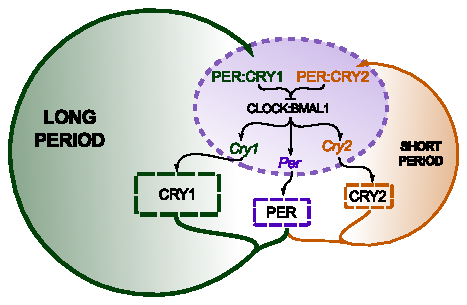
\includegraphics[width=0.8\textwidth]{chap2/figures/twoloops_noopacity.pdf}
  \titlecaption{Connectivity of \fref{mod:hirota}}{
    Schematic for the core negative feedback loop, consisting of the two redundant {\it Cry} mechanisms. 
  The wild-type period, consisting of both loops, is a balance between the short and long oscillations.} \label{fig:twoloops}
\end{figure}

\subsubsection{The CRY1/CRY2 ratio}
{\it In silico} modeling was used to test the feasibility of the above hypothesis, and to investigate possible mechanisms by which the CRY1/CRY2 ratio might control the period of oscillations. 
The model uses eight state variables for the three mRNA species ({\it Per}, {\it Cry1}, and {\it Cry2}), three cytosolic proteins, and two nuclear proteins. 
The differential equations for each state were formulated using standard Hill-type repression, Michaelis-Menten, and mass action kinetics. 
The 21 unknown kinetic parameters were found by fitting the stoichiometric data from \cite{Lee2001} using a genetic algorithm approach, requiring correct periods for the $\text{\it Cry1}^{-/-}$  and $\text{\it Cry2}^{-/-}$  knockouts.

I investigated two possible mechanisms to explain the long/short period phenotype of the CRY1/CRY2 loops. 
First, following experimental evidence, I allowed CRY1 and CRY2 to have different inhibitory efficiency \cite{GriffinJr.1999}. 
However, optimizations with this structure were unable to find a parameter set with appropriate period sensitivities, described in \fref{sec:parameter}. 
Instead, I investigated whether the difference in potency between {\it Crys} could be explained through difference in degradation rates. 
To this end, I allowed the degradation rates of nuclear CRY1 and CRY2 to differ, while holding their inhibition constants equal. 
Using this configuration, the structure was able to fit the experimental sensitivities. 
In the optimized parameter set, the degradation rate of nuclear CRY2 is higher than that of CRY1, such that for a constant total nuclear CRY, higher fractions of CRY2 cause the repressive complexes to be cleared faster. 
Since PER is the limiting reagent in nuclear entry, the amount of total CRY that enters the nucleus is largely insensitive to perturbations in cytosolic CRY expression. 
In effect, the two isoforms of CRY must compete for the available PER, and thus the nuclear CRY1/CRY2 levels are constrained with a ratio proportional to their relative expression. 
The period of the clock is thus governed by the nuclear CRY1/CRY2 ratio, where higher amounts of {\it Cry1} shift the clock closer to the $\text{\it Cry2}^{-/-}$ phenotype, and higher amounts of {\it Cry2} shift the clock closer to the $\text{\it Cry1}^{-/-}$ phenotype. 
\Fref{fig:nucleartimecourse} shows the time varying total complex concentration under various perturbations, with the relative contributions from CRY1 and CRY2 highlighted.

\begin{figure}[bt]
  \centering
  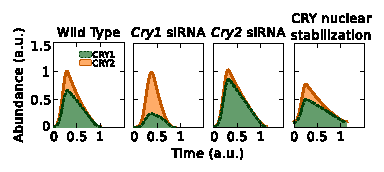
\includegraphics[width=0.8\textwidth]{chap2/figures/nucleartimecourse.pdf}
  \titlecaption{Repressor degradation profiles}{
    Time course plots of the simulated total nuclear repressor concentration for the degradation model under various clock conditions. 
    The relative contribution of CRY1 and CRY2 are shaded green and orange, respectively. 
  Longer periods occur when a higher percentage of the nuclear complex is CRY1, taking longer to degrade.}
  \label{fig:nucleartimecourse}
\end{figure}

\subsubsection{Model equations}
The model is formulated as set of 8 ordinary differential equations shown in \fref{mod:hirota} (for the degradation-based model) and \fref{mod:actfns} (for the activation-based model). 
Additional assumptions made while formulating the model equations are listed below:

\begin{itemize}

  \item For simplicity and  ease of parameter estimation, the model only considers the three genes {\it Per}, {\it Cry1}, and {\it Cry2}, not explicitly considering the three known isoforms of {\it Per}. 

  \item EBOX activators {\it Clock} and {\it Bmal1} are considered constitutively expressed and are represented by the $v_{\text{txn}}$ parameters. 

  \item Repression of CLOCK-BMAL1 activity is attained through Hill-type inhibition. The Hill coefficient is fixed at 3, which was found to provide sufficient nonlinearity for oscillations. See below for the derivation of the repressor input function used in \fref{mod:hirota} and \fref{mod:actfns}.

  \item The degradation of the mRNA species and cytoplasmic proteins is assumed to follow standard Michaelis-Menten kinetics.

  \item The degradation kinetics of the nuclear proteins are assumed to follow Michaelis-Menten kinetics. Because both $\bm{C1N}$ and $\bm{C2N}$ are thought to be degraded by the same pathway in the nucleus, kinetic equations using the {\it pseudo} steady-state hypothesis were derived for two substrates sharing the same enzyme. As a result, each CRY isoform acts as an inhibitor to the other's degradation. This mechanism is summarized in \fref{fig:shareddeg}.
\end{itemize}

\begin{figure}[tbp]
  \centering
  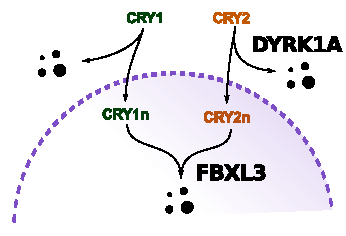
\includegraphics{chap2/figures/cryseperatedegradation.pdf}
  \titlecaption{Degradation of both CRY isoforms is regulated by the same enzyme}{In developing the model equations for \fref{mod:hirota}, a key assumption was that both isoforms of Cryptochrome were degraded by the same enzyme. Without such a scheme, the shortest periods were obtained by maximizing degradation through equal nuclear entry of both isoforms.}
  \label{fig:shareddeg}
\end{figure}

\begin{model}[p]
  \centering
  \titlecaption{A degradation-based model of the core feedback loop}{Lower case letters (p: {\it Per}, c1: {\it Cry1}, c2: {\it Cry2}) are mRNA state variables. Uppercase letters (P: PER, C1: CRY1, C2: CRY2) are the free (cytosolic) proteins. C1N: CRY1 and C2N: CRY2 are the nuclear proteins.}

  \begin{align}
    \label{eq:p}
    \frac{d\mathrm{\bf p}}{dt}    & = \frac{v_{\text{txn,{\bf p}}}}{k_{\text{txn,{\bf p}}} + \left(\text{\bf C1N} + \text{\bf C2N} \right)^3} - \frac{v_{\text{deg,{\bf p}}} \;\text{\bf p} }{k_{\text{deg,{\bf p}}} +\text{\bf p} } \\
        %
    \label{eq:c1}
    \frac{d\text{\bf c1}}{dt}   & = \frac{v_{\text{txn,{\bf c1}}}}{k_{\text{txn,{\bf c}}} + \left(\text{\bf C1N} + \text{\bf C2N} \right)^3} - \frac{v_{\text{deg,{\bf c1}}} \;\text{\bf c1} }{k_{\text{deg,{\bf c}}} +\text{\bf c1} } \\
        %
    \label{eq:c2}
    \frac{d\text{\bf c2}}{dt}   & = \frac{v_{\text{txn,{\bf c2}}}}{k_{\text{txn,{\bf c}}} + \left(\text{\bf C1N} + \text{\bf C2N} \right)^3} - \frac{v_{\text{deg,{\bf c2}}} \;\text{\bf c2} }{k_{\text{deg,{\bf c}}} +\text{\bf c2} } \\
        %
    \begin{split}
      \frac{d\text{\bf P}}{dt}  & = k_\text{tln,{\bf p}} \;\text{\bf p}  - \frac{v_{\text{deg,{\bf P}}} \;\text{\bf P} }{k_{\text{deg,{\bf P}}} +\text{\bf P} } - v_{\text{a,{\bf CP}}} \;\text{\bf P}  \;\text{\bf C1}  + v_{\text{d,{\bf CP}}} \;\text{\bf C1N} \\
      & \quad - v_{\text{a,{\bf CP}}} \;\text{\bf P}  \;\text{\bf C2}  + v_{\text{d,{\bf CP}}} \; \text{\bf C2N}
    \end{split} \\
        %
    \frac{d\text{\bf C1}}{dt}   & =\text{\bf c1}  - \frac{v_{\text{deg,{\bf C1}}} \;\text{\bf C1} }{k_{\text{deg,{\bf C}}} +\text{\bf C1} } - v_{\text{a,{\bf CP}}} \;\text{\bf P}  \;\text{\bf C1}  + v_{\text{d,{\bf CP}}} \;\text{\bf C1N} \\
        %
    \frac{d\text{\bf C2}}{dt}   & =\text{\bf c2} - \frac{ v_{\text{deg,{\bf C2}}} \;\text{\bf C2} }{k_{\text{deg,{\bf C}}} +\text{\bf C2} } - v_{\text{a,{\bf CP}}} \;\text{\bf P}  \;\text{\bf C2}  + v_{\text{d,{\bf CP}}} \; \text{\bf C2N} \\
        %
    \frac{d\text{\bf C1N}}{dt}  & = - \frac{ v_{\text{deg,{\bf CP}}} \;\text{\bf C1N} }{k_{\text{deg,{\bf CP}}} +\text{\bf C1N}  + \text{\bf C2N} } + v_{\text{a,{\bf CP}}} \;\text{\bf P}  \;\text{\bf C1} - v_{\text{d,{\bf CP}}} \;\text{\bf C1N} \\
        %
    \label{eq:C2N}
    \frac{d\text{\bf C2N }}{dt} & = - \frac{ \left(v_{\text{deg,{\bf CP}}} \; m_{\text{\bf C2N}}\right) \; \text{\bf C2N} }{k_{\text{deg,{\bf CP}}} + \text{\bf C2N}  +\text{\bf C1N} } + v_{\text{a,{\bf CP}}} \;\text{\bf P}  \;\text{\bf C2} - v_{\text{d,{\bf CP}}} \; \text{\bf C2N}
  \end{align}
  \label{mod:hirota}
\end{model}


\begin{model}[p]
  \centering
  \titlecaption{Changed equations for the activation-based model}{The remainder of the model equations (not duplicated below) are found in  \fref{mod:hirota}}

  \begin{align*}
    \frac{d\text{\bf p}}{dt} &= \frac{v_{\text{txn,{\bf p}}}}{k_{\text{txn,{\bf p}}} + \left(m_{\text{\bf C2N}} \; \text{\bf C1N}  + \text{\bf C2N} \right)^3} - \frac{v_{\text{deg,{\bf p}}} \;\text{\bf p} }{k_{\text{deg,{\bf p}}} +\text{\bf p} } \tag{$\ref{eq:p}^{\star}$}\\
        %
    \frac{d\text{\bf c1}}{dt} &= \frac{v_{\text{txn,{\bf c1}}}}{k_{\text{txn,{\bf c}}} + \left(m_{\text{\bf C2N}} \; \text{\bf C1N}  + \text{\bf C2N} \right)^3} - \frac{v_{\text{deg,{\bf c1}}} \;\text{\bf c1} }{k_{\text{deg,{\bf c}}} +\text{\bf c1} } \tag{$\ref{eq:c1}^{\star}$}\\
        %
    \frac{d\text{\bf c2}}{dt} &= \frac{v_{\text{txn,{\bf c2}}}}{k_{\text{txn,{\bf c}}} + \left(m_{\text{\bf C2N}} \; \text{\bf C1N}  + \text{\bf C2N} \right)^3} - \frac{v_{\text{deg,{\bf c2}}} \;\text{\bf c2} }{k_{\text{deg,{\bf c}}} +\text{\bf c2} } \tag{$\ref{eq:c2}^{\star}$}\\
        %
    \frac{d\text{\bf C2N }}{dt} &= - \frac{ v_{\text{deg,{\bf CP}}} \; \text{\bf C2N} }{k_{\text{deg,{\bf CP}}} + \text{\bf C2N}  +\text{\bf C1N} } + v_{\text{a,{\bf CP}}} \;\text{\bf P}  \;\text{\bf C2} - v_{\text{d,{\bf CP}}} \; \text{\bf C2N}
    \tag{$\ref{eq:C2N}^{\star}$}
  \end{align*}
  \label{mod:actfns}
\end{model}


\begin{table}[p]
  \titlecaption{Parameter values for \fref{mod:hirota}}{Parameters for model described in \fref{mod:hirota}.}
  \label{tab:parset}
  \vspace{2mm}
  \centering
  \begin{tabular}{cllrr} \toprule
    & Parameter                 & Description                       & Degradation & Activation \\ \midrule
    1  & $v_{\text{txn,{\bf p}}}$  & {\it Per} Transcription rate      & 0.195       & 0.276 \\
    2  & $v_{\text{txn,{\bf c1}}}$ & {\it Cry1} Transcription rate     & 0.131       & 0.062 \\
    3  & $v_{\text{txn,{\bf c2}}}$ & {\it Cry1} Transcription rate     & 0.114       & 0.053 \\
    4  & $k_{\text{txn,{\bf p}}}$  & {\it Per} Repression constant     & 0.425       & 0.425 \\
    5  & $k_{\text{txn,{\bf c}}}$  & {\it Cry1/2} Repression constant  & 0.259       & 0.262 \\
    6  & $v_{\text{deg,{\bf p}}}$  & {\it Per} Max degradation rate    & 0.326       & 0.472 \\
    7  & $v_{\text{deg,{\bf c1}}}$ & {\it Cry1} Max degradation rate   & 0.676       & 0.322 \\
    8  & $v_{\text{deg,{\bf c2}}}$ & {\it Cry2} Max degradation rate   & 0.608       & 0.290 \\
    9  & $k_{\text{deg,{\bf p}}}$  & {\it Per} Degradation constant    & 0.011       & 0.024 \\
    10 & $k_{\text{deg,{\bf c}}}$  & {\it Cry1/2} Degradation constant & 1.149       & 0.809 \\
    11 & $v_{\text{deg,{\bf P}}}$  & Max PERc degradation rate         & 2.970       & 2.970 \\
    12 & $k_{\text{deg,{\bf P}}}$  & PERc degradation constant         & 0.034       & 0.034 \\
    13 & $v_{\text{deg,{\bf C1}}}$ & Max CRY1c degradation rate        & 1.523       & 1.048 \\
    14 & $v_{\text{deg,{\bf C2}}}$ & Max CRY2c degradation rate        & 1.686       & 1.134 \\
    15 & $k_{\text{deg,{\bf C}}}$  & CRYc degradation constant         & 2.017       & 2.028 \\
    16 & $v_{\text{deg,{\bf CP}}}$ & CRYn degradation rate             & 0.101       & 0.070 \\
    17 & $m_{\text{\bf C2N}}$      & CRY2n degradation multiplier      & 3.318       & 3.334 \\
    18 & $k_{\text{deg,{\bf CP}}}$ & CRYn degradation constant         & 0.053       & 0.053 \\
    19 & $v_{\text{a,{\bf CP}}}$   & CRYn association rate             & 0.041       & 0.028 \\
    20 & $v_{\text{d,{\bf CP}}}$   & CRYn dissociation rate            & 0.002       & 0.001 \\
    21 & $k_{\text{tln,{\bf p}}}$  & PER translation rate              & 3.000       & 1.000 \\ \bottomrule
    \hline
  \end{tabular}
\end{table}


\subsubsection{Derivation of a shared enzyme degradation rate}

To find the rate equations associated with a shared-enzyme degradation mechanism, we derive them from the equilibrium relationships:
\begin{equation*}
  \text{[E]} + \text{[S1]} \xrightleftharpoons[k_{-1}]{k_1} \text{[ES1]} \xrightarrow{k_{d,1}} \text{[E]}
\end{equation*}
\begin{equation*}
  \text{[E]} + \text{[S2]} \xrightleftharpoons[k_{-2}]{k_2}  \text{[ES2]} \xrightarrow{k_{d,2}} \text{[E]}
\end{equation*}
\begin{equation} \label{eq:totE}
  [\text{E}_t] = \text{[E]} + \text{[ES1]} + \text{[ES2]}
\end{equation}
The end goal is the degradation rates of the two enzyme complexes:
\begin{align}
  \begin{split}\label{eq:r1}
    r_{d,1} &= k_{d,1} \ \text{[ES1]}\\
    r_{d,2} &= k_{d,2} \ \text{[ES2]}
  \end{split}
\end{align}
As was done in \fref{sec:mmenten}, we invoke the standard pseudo steady-state assumption and set $\nicefrac{d[\text{ES}]}{dt}=0$, and obtain the following production = consumption equalities for [ES1]:
\begin{equation} \label{eq:pss}
  k_1\text{[E]}\text{[S]} = k_{-1}\text{[ES1]} + k_{d,1}\text{[ES1]}
\end{equation}
Solving \fref{eq:pss} for ES1 and substituting in \fref{eq:totE}, we obtain
\begin{equation*}
  \left(\frac{k_{-1}+k_{d,1}}{k_1}\right)\text{[ES1]} = \left([\text{E}_t] - \text{[ES1]} - \text{[ES2]}\right)\text{[S1]}
\end{equation*}
After defining a useful combined rate constant,
\begin{equation*}
  K_1 \equiv \frac{k_{-1}+k_{d,1}}{k_1}
\end{equation*}
we can further simplify
\begin{align}
  K_1 \text{[ES1]} + \text{[S1]}\text{[ES1]} &= ([\text{E}_t] - [\text{ES2}])[\text{S1}] \notag\\
    %
  [\text{ES1}] &= \frac{([\text{E}_t] - [\text{ES2}])[\text{S1}]}{K_1 + [\text{S1}]} \label{eq:eqabove}
\end{align}
If we perform the same operations for [ES2] and plug them into \fref{eq:eqabove}.
\begin{align}
  [\text{ES1}] &= \frac{\left(\text{E}_t] - \frac{([\text{E}_t] - [\text{ES1}])[\text{S2}]}{K_2 + [\text{S2}]}\right)\text{S1}]}{K_1 + [\text{S1}]} \notag\\
  [\text{ES1}] &= \frac{\text{[E]}_t \text{[S1]}}{K_1 + \text{[S1]}} - \frac{\text{[E]}_t \text{[S1]} \text{[S2]}}{(K_1 + \text{[S1]}) (K_2 + \text{[S2]})} + \frac{\text{[ES1]} \text{[S1]} \text{[S2]}}{(K_1 + \text{[S1]}) (K_2 + \text{[S2]})} \notag\\
  \label{eq:twofracs}
  [\text{ES1}] &= \left(\frac{\text{[E]}_t \text{[S1]}}{K_1 + \text{[S1]}}\right) \left(\frac{1 - \frac{\text{[S2]}}{K_2 + \text{[S2]}}}{1 - \frac{\text{[S1]} \text{[S2]}}{(K_1 + \text{[S1]}) (K_2 + \text{[S2]})}}\right)
\end{align}
If we pull the second fraction from \fref{eq:twofracs} into the denominator of the first, we can simplify further.
\begin{align*}
  [\text{ES1}] &= \frac{\text{[E]}_t \text{[S1]}}{\left(\frac{K_1 + \text{[S1]} - \frac{\text{[S1]} \text{[S2]}}{K_2 + \text{[S2]}}}{1 - \frac{\text{[S2]}}{K_2 + \text{[S2]}}}\right)} \\
  [\text{ES1}] &= \frac{\text{[E]}_t \text{[S1]}}{\left(\frac{K_2 + \text{[S2]}}{K_2}\right) \left(K_1 + \text{[S1]} - \frac{\text{[S1]} \text{[S2]}}{K_2 + \text{[S2]}}\right)} \\
  [\text{ES1}] &= \frac{K_2 \text{[E]}_t \text{[S1]}}{(K_1 + \text{[S1]})(K_2 + \text{[S2]}) - \text{[S1]}\text{[S2]}} \\
  [\text{ES1}] &= \frac{K_2 \text{[E]}_t \text{[S1]}}{K_1 K_2 + K_2\text{[S1]} + K_1\text{[S2]}} \\
  [\text{ES1}] &= \frac{K_2 \text{[E]}_t \text{[S1]}}{K_1 K_2 + K_2\text{[S1]} + K_1\text{[S2]}}
\end{align*}
Dividing top and bottom by K2:
\begin{equation}
[\text{ES1}] = \frac{\text{[E]}_t \text{[S1]}}{K_1 + \text{[S1]} + \frac{K_1}{K_2}\text{[S2]}}\label{eq:es1}
\end{equation}
Substituting \fref{eq:es1} into \fref{eq:r1} and setting $K_1 = K_2$, $k_{d,1} \neq k_{d,2}$, we obtain the final shared rate laws (with an equivalent analysis for [ES2])
\begin{align*}
  r_{d,1} &= \frac{V_\text{max,1} \text{[S1]}}{K_M + \text{[S1]} + \text{[S2]}} \\ \\
  r_{d,2} &= \frac{V_\text{max,2} \text{[S2]}}{K_M + \text{[S1]} + \text{[S2]}}
\end{align*}

\subsubsection{Derivation of Hill-type repression formulas}
To derive the equations for the Hill-type inhibition, allowing for different repressive activities (\fref{mod:actfns}), we start with the standard equation for Hill-type regulation:
\begin{equation} \label{eq:htr}
  \frac{v_{\text{max}}[A]^n}{K_m^n + [A]^n}
\end{equation}
Allowing for competitive inhibition with two inhibitors, $K_m$ is replaced with the apparent Michaelis-Menten constant
\begin{equation}\label{eq:kmapp}
  K_m^{\text{app}} = K_m \left(1 + \frac{[I_1]}{K_{i,1}} + \frac{[I_2]}{K_{i,2}}\right)
\end{equation}
By assuming constitutive activator concentrations and non-dimensionalizing $[I^{\star}] = \frac{[I]}{K_{i,2}}$, $m = \frac{K_{i,2}}{K_{i,1}}$:
\begin{equation*}
  \frac{v_{\text{max}^{\star}}}{K_m^{\star} + \left(m \; [I^{\star}_1] + [I^{\star}_2]\right)^n}
\end{equation*}
Assuming equal repressive activity $(K_{i,2} = K_{i,1})$, $m = 1$, we obtain the rate equation used in the degradation model.


\subsection{Parameter estimation}\label{sec:parameter}
The model equations, specifying the state and parameter dependent time derivatives of each concentration variable, were written in python using the CasADi computer algebra package \cite{Andersson2010}. 
The model was simulated using the SUNDIALS suite of ODE solvers \cite{Hindmarsh2005}. 
A parameter-dependent cost function was developed that assigns numerical values reflecting how well a parameter set fits desired features, taken from \cite{Lee2001}. 
The first step in the cost function evaluation is the numerical solution of the limit cycle, described previously \cite{Wilkins2009}. 
If a limit cycle was unable to be found, the cost function returns a maximum value. 
Otherwise, the cost function returns a squared difference from the desired value. 
A priority weight was also attached to each cost entry, such that more important costs would be prioritized. 
A description of each entry in the cost function, along with the value for experimental and final model is shown in \fref{tab:cost} (degradation-based model, \fref{mod:hirota}; activation-based model, \fref{mod:actfns}). 
To minimize the cost function, we employed a genetic algorithm method used previously for optimizing circadian parameters \cite{Mirsky2009}. 
In the method, 5000 solutions are calculated at random parameter values within feasible bounds. 
Those with the best cost function scores are kept and used to generate subsequent solutions. 
This procedure is iterated for up to 2000 generations, or until convergence criteria are met.

\begin{longtable}{cp{6.0cm}crrr}
  \titlecaption{Summary of cost function entries}{
    The weights for each entry were chosen based on the relative importance of the desired behavior. 
    Entries 1-9 and 12-16 were obtained from the data presented in \cite{Lee2001}. 
    SiRNA sensitivities were obtained were taken from \cite{Zhang2009}.}\\ \toprule \label{tab:cost} 
    & Description & Weight & Desired & Degradation & Activation \\
    \midrule
  \endfirsthead

  \toprule
  & Description & Weight & Desired & Degradation & Activation \\
  \midrule
\endhead

\bottomrule
\endfoot
1 & {\it per} mRNA peak-trough ratio
$$\frac{y_\text{max}(\text{\it Per})}{y_\text{min}(\text{\it Per})}$$
& 0.5 & $> 20$ & large & large \\
%
2 & {\it Cry1} mRNA peak-trough ratio 
$$\frac{y_\text{max}(\text{\it Cry1})}{y_\text{min}(\text{\it Cry1})}$$
& 0.5 & $2.155$ &  8.942 & 3.748\\
%
3 & {\it Cry2} mRNA peak-trough ratio 
$$\frac{y_\text{max}(\text{\it Cry2})}{y_\text{min}(\text{\it Cry2})}$$
& 0.5 & $2.236$ &  7.813 & 3.484\\
%
4 & PER protein peak to trough ratio 
$$\frac{y_\text{max}(\text{PER})}{y_\text{min}(\text{PER})}$$
& 5 & $> 20$ & large & large\\
%
5 & CRY1 protein peak-trough ratio 
$$\frac{y_\text{max}(\text{CRY1})}{y_\text{min}(\text{CRY1})}$$
& 3 & $3.247$ & 6.385 & 1.847\\
%
6 & CRY2 protein peak-trough ratio 
$$\frac{y_\text{max}(\text{CRY2})}{y_\text{min}(\text{CRY2})}$$
& 3 & $1.975$ & 8.094 & 2.347 \\
%
7 & Fraction PER of total protein 
$$\frac{y_\text{max}(\text{PER})}{y_\text{max}(\text{PER}) + y_\text{max}(\text{CRY1}) + y_\text{max}(\text{CRY2})}$$
& 3 & $0.105$ & 0.169 & 0.073 \\
%
8 & Fraction CRY1 of total protein 
$$\frac{y_\text{max}(\text{CRY1})}{y_\text{max}(\text{PER}) + y_\text{max}(\text{CRY1}) + y_\text{max}(\text{CRY2})}$$
& 3 & $0.555$ & 0.473 & 0.554 \\
%
9 & Fraction CRY2 of total protein 
$$\frac{y_\text{max}(\text{CRY2})}{y_\text{max}(\text{PER}) + y_\text{max}(\text{CRY1}) + y_\text{max}(\text{CRY2})}$$
& 3 & $0.341$ & 0.358 & 0.373 \\
%
10 & {\it Cry1} siRNA period sensitivity 
$$\frac{\partial T}{\partial v_{\text{deg,{\bf c1}}}}$$
& 5 & $< 0$ & $< 0$ & $> 0$ \\
%
11 & {\it Cry2} siRNA period sensitivity 
$$\frac{\partial T}{\partial v_{\text{deg,{\bf c2}}}}$$
& 5 & $> 0$ & $> 0$ & $< 0$ \\
%
12 & {\it Cry1} knockout period 
$$\frac{T(\text{\it Cry1}^{-/-})}{T(\text{WT})}$$
& 5 & $< 95 \%$ & $92.1 \%$ & $193.4 \%$ \\
%
13 & {\it Cry2} knockout period 
$$\frac{T(\text{\it Cry2}^{-/-})}{T(\text{WT})}$$
& 5 & $> 115 \%$ & $131.8 \% $ & $99.4 \%$ \\
%
14 & Fraction CRY1 entering nucleus 
$$\frac{y_\text{max}(\text{CRY1}_n)}{y_\text{max}(\text{CRY1} + \text{CRY1}_n)}$$
& 1 & $0.40$ & $0.195$ & 0.059 \\
%
15 & Fraction CRY2 entering nucleus 
$$\frac{y_\text{max}(\text{CRY2}_n)}{y_\text{max}(\text{CRY2} + \text{CRY2}_n)}$$
& 1 & $0.35$ & $0.139$ & 0.059 \\
%
16 & Time delay between nuclear repressors and mRNA 
$$t_\text{max}(\text{nuclear protein}) - t_\text{max}(\text{mRNA})$$
& 3 & $75 \%$ & $0.850$ & 0.848 \\
%
17 & Time delay between mRNA and cytoplasmic protein
$$t_\text{max}(\text{mRNA}) - t_\text{max}(\text{protein})$$ 
& 3 & $25 \%$ & $0.057$ & 0.095 \\
%
18 & Time delay between cytoplasmic protein and nuclear protein
$$t_\text{max}(\text{protein}) - t_\text{max}(\text{nuclear protein})$$
& 3 & $0 \%$ & $0.093$ & 0.057 \\
\end{longtable}

\subsection{Model validation and dynamics}
The model was validated by comparing the simulated dynamics to experimental measurements. 
First, the time course plots of the state variables display reasonable phases and amplitudes, and oscillate with a period of 23.7 hours (\fref{fig:timecourse}). 
The knockout periods are 21.7 hr ($91.4\%$ of WT) for $\text{\it Cry1}^{-/-}$  and 31.5 hr ($133\%$ of WT) for $\text{\it Cry2}^{-/-}$, indicating that the two feedback loops are indeed redundant with different free-running periods.

\begin{figure}[bt]
  \centering
  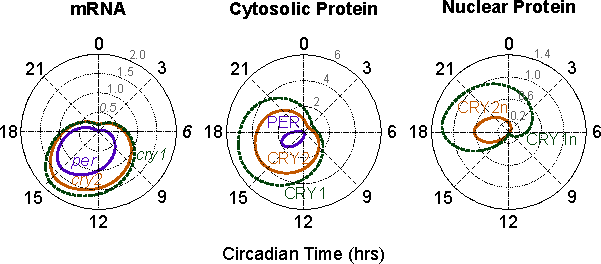
\includegraphics[width=0.8\textwidth]{chap2/figures/timecourse.pdf}
  \titlecaption{Time course concentration profiles of \fref{mod:hirota}}{
    The three polar plots show the time-varying levels of each clock component for optimal parameter set. 
    In these plots, the amplitude of each variable (always positive) is plotted against its phase, $0 \rightarrow 2\pi$. 
    Since the limit cycle is periodic, this results in a closed curve. 
    Rising mRNA levels caused by low repressor concentrations (CT12) result in accumulating cytosolic protein (left plot). 
    Lower levels of PER prevent all the available CRY from entering the nucleus (middle plot). 
  High levels of nuclear repressors halt transcription until both CRYs have degraded (right plot).}
  \label{fig:timecourse}
\end{figure}

\subsubsection{SiRNA knockdowns}
SiRNA knockdowns were performed {\it in silico} by increasing the degradation rate for the corresponding mRNA (\fref{fig:experimentalvalidation}), as done previously in \cite{Relogio2011}. 
{\it Cry1} and {\it Cry2} knockdowns in wild type conditions show close agreement to experiment \cite{Zhang2009}, and demonstrate that altering the nuclear CRY1/CRY2 ratio is effective in changing the period of oscillation.

\subsubsection{CRY2 cytosolic stabilization}
The {\it Dyrk1a} knockdown in \cite{Kurabayashi2010} serves as another demonstration of the change in period as a response to a change in nuclear CRY1/CRY2 ratio. 
To demonstrate the effect in silico, the degradation rate of cytosolic CRY2 was decreased. 
Matching experimental evidence, the cytosolic CRY2 levels rose, with a corresponding change in the nuclear CRY ratio and decrease in period.

\subsubsection{Single cry perturbations}
The $\text{\it Cry1}^{+/-}$ $\text{\it Cry2}^{-/-}$ and $\text{\it Cry1}^{-/-}$ $\text{\it Cry2}^{+/-}$ single/double knockout perturbations from \cite{VanderHorst1999} were approximated with an appropriate knockout and siRNA knockdown, and show the correct period shortening. 
With one {\it Cry} knocked out, the levels of cytoplasmic PER are no longer stoichiometrically limiting. 
In this case, less {\it Cry} leads to less nuclear complex, which is cleared faster.

\begin{figure}[bt]
  \centering
  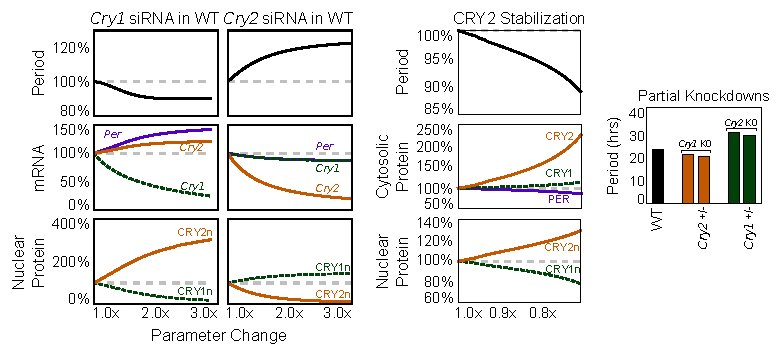
\includegraphics[width=\textwidth]{chap2/figures/experimentalvalidation.pdf}
  \titlecaption{Model validation against experimental results}{
    When comparing against existing experimental results, the model shows the correct response for {\it Cry1} siRNA, {\it Cry2} siRNA, and $\text{CRY}_c$ stabilization (left, middle), through an adjustment in the nuclear CRY1/CRY2 ratio. 
    The model also correctly captures the single/double knockout phenotype of \cite{VanderHorst1999}, (right)} \label{fig:experimentalvalidation}
\end{figure}

\subsection{Prediction of KL001 mechanism}
Using the completed model, I investigated possible mechanisms by which KL001 might lengthen the circadian period. 
Experimental evidence indicates that stabilization of CRY can either lengthen the period ({\it Fbxl3} knockdown) or shorten the period ({\it Dyrk1a} knockdown). 
Assuming equal effect on both isoforms of CRY, the model confirms that cytoplasmic stabilization results in period shortening, since excess CRY expedites the nuclear import of the PER:CRY repressive complex. 
However, stabilizing nuclear CRY (\fref{fig:nucleartimecourse}, last column) yields the appropriate period lengthening observed experimentally. 
We therefore predicted that KL001 acts primarily in the nucleus, potentially through the FBXL3 degradation pathway. 
Additionally, the model predicts that the compound’s effect on $\text{\it Cry1}^{-/-}$ and $\text{\it Cry2}^{-/-}$ systems would be similar to its effect on the wild type clock, causing dose-dependent period lengthening (\fref{fig:40662prediction}, left and right).


\begin{figure}[bt]
    \centering
    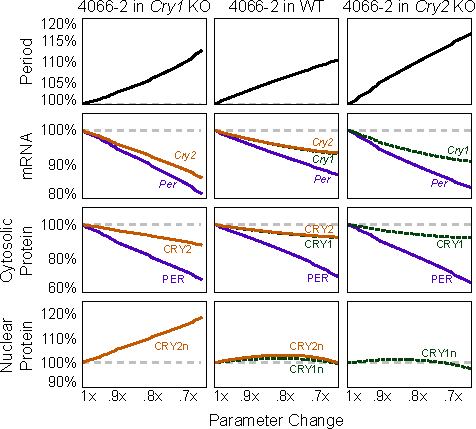
\includegraphics[width=0.7\textwidth]{chap2/figures/prediction.pdf}
    \titlecaption{Prediction of the KL001 mechanism}{ {\it In silico} response to equal stabilization of both CRYs in the nucleus results in longer periods (middle column), matching observed results. The model correctly predicts that stabilization of individual CRYs in the knockout environments also causes period lengthening.}
    \label{fig:40662prediction}
\end{figure}

\subsubsection{Experimental confirmation}
Experimental tests of the model's predictions were performed. 
Nuclear CRY1 and CRY2 levels were up-regulated and almost sustained, respectively, while PER1 level was strongly down-regulated by the compound, supporting stabilization of nuclear CRY, the predicted mechanism. 
Additionally, continuous treatment with KL001 lengthened the period in both {\it Cry1} and {\it Cry2} knockout cells in a dose-dependent manner. 
Similarly, the compound caused period lengthening in both CRY1 and CRY2 knockdown U2OS cells. 
We further investigated the effect of KL001 in SCN explants, which show robust rhythms even in the absence of {\it Cry1}, due to intercellular coupling \cite{Liu2007}. 
Both {\it Cry1} and {\it Cry2} knockout SCN exhibited dose-dependent period lengthening by the compound treatment. 
Thus, in a single {\it Cry} knockout, stabilization of either nuclear CRY1 and CRY2 causes period lengthening, confirming model predictions.
Furthermore, the period-lengthening response of KL001 was abolished in cells treated with FBXL3 siRNA, further confirming that the period effect of KL001 is mediated by inhibiting FBXL3-CRY interactions (\fref{fig:fbxl3data}).
This prediction was further verified in subsequent structural biology work \cite{Nangle2013}.

\begin{figure}[tbp]
  \centering
  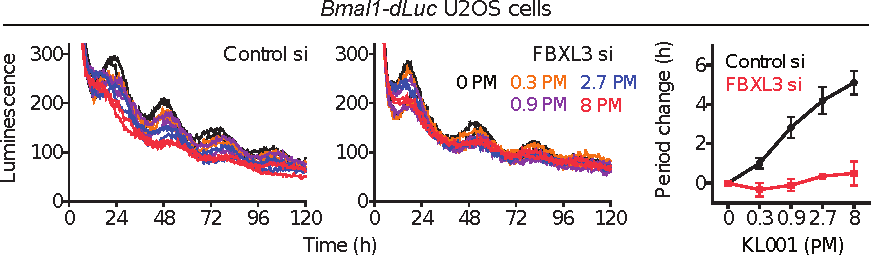
\includegraphics{chap2/figures/fbxl3kl001data.pdf}
  \titlecaption{FBXL3 knockdown interferes with period-lengthening effect of KL001}{The dose-dependent period increase of KL001 (right, black line) is abolished in cells treated with FBXL3 siRNA, indicating the mechanism of KL001 acts through FBXL3 and confirming model predictions}
  \label{fig:fbxl3data}
\end{figure}

\begin{figure}[p]
  \centering
  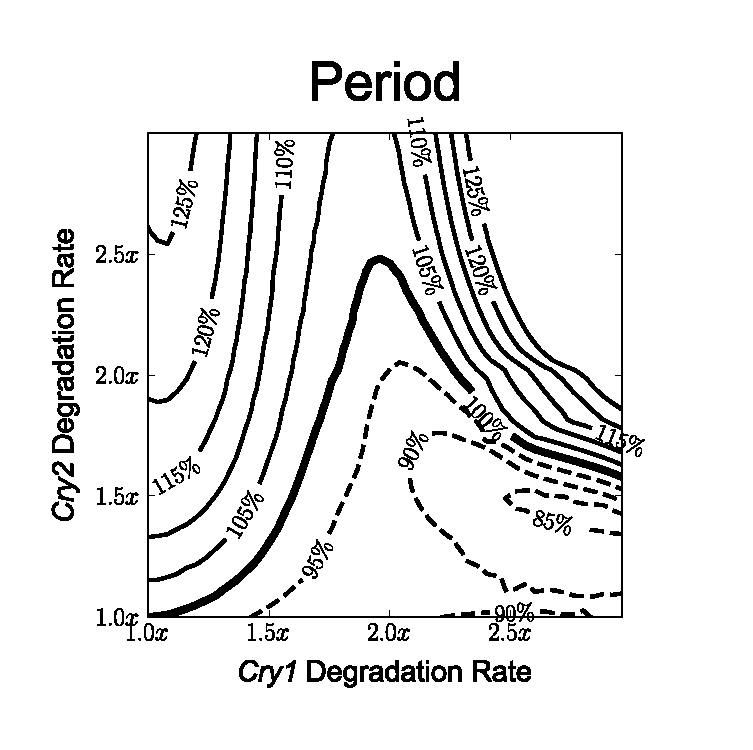
\includegraphics[width=0.5\textwidth]{chap2/figures/crysimultaneousknockdown.pdf}
  \titlecaption{Simultaneous knockdown of {\it Cry1} and {\it Cry2}}{Period contours (\% change) resulting from simultaneous {\it in silico} siRNA knockdowns of {\it Cry1} (x-axis) and {\it Cry2} (y-axis). The plot shows that the CRY1/CRY2 ratio determines the period, independent of total CRY, for perturbations up to twice the normal mRNA degradation rate.}
  \label{fig:simultaneouskdown}
\end{figure}

\begin{figure}[p]
  \centering
  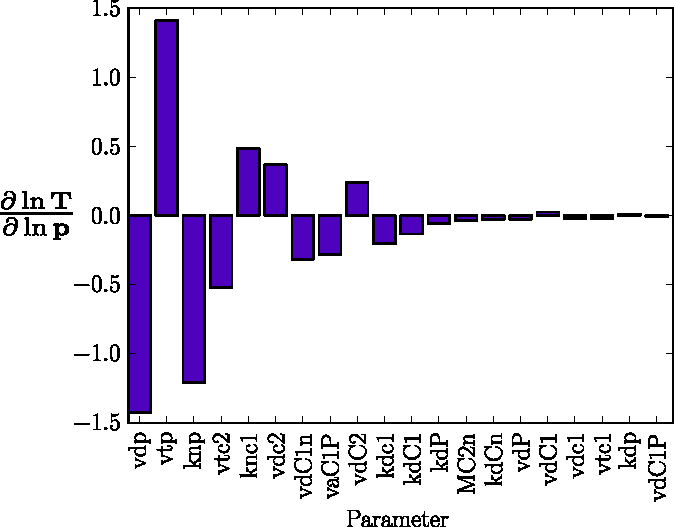
\includegraphics[width=0.6\textwidth]{chap2/figures/firstordersens.pdf}
  \titlecaption{First order relative period sensitivities}{ Dimensionless period sensitivities with respect to the kinetic parameters in the degradation-based model. Perturbations to most clock rates result in noticeable changes to the free-running period. Many of the most sensitive parameters are transcriptional rates, which can be easily changed through mutation of DNA promoter regions.}
  \label{fig:firstordersens}
\end{figure}

\section{Discussion}
\subsection{Insights into circadian network design}
Mathematical modeling has revealed how the balancing of two redundant feedback loops can provide fine control over the oscillatory period. 
A contour plot of period vs CRY1 or CRY2 abundance is shown in \fref{fig:simultaneouskdown}, which shows that the model's period is largely insensitive to the total amount of CRY ($45^\circ$ line), but highly dependent on the ratio of the two isoforms. 
Sensitivity analysis of our mathematical model (\fref{fig:firstordersens}) reveals that subtle changes in most of the involved rates can have an effect on the clock's free running period, which could be caused by evolutionary noise. 
Since many studies have linked entrainment to non-natural periods with long-term health problems, a mechanism to align the clock’s natural period to that of the environment would be advantageous. 
It is therefore possible that the period control afforded by CRY1/CRY2 balancing is a deliberately conserved design principle of the circadian clock, which confers period robustness against random mutations of clock components. 
Indeed, the presence of independent control of the cytosolic CRY2 levels suggests that the biological clock can control its period through simple post-translational modifications \cite{Kurabayashi2010}. 

\subsection{Identifiability of model parameters}
Due to the high dimensionality of the model equations and sparsity of the experimental data, it is likely that more than one set of parameters would fit the cost function defined in \fref{tab:cost}. 
While the fact that {\itshape any} parameter set for the given model equations reproduces experimental results is enough to confirm that our hypothesized mechanism is mathematically consistent, we must be careful in placing too much confidence in predictions based on the particular parameter set generated by the optimization algorithm. 
While subsequent experimental results confirm many of our model predictions, a more rigorous exploration of parameter space would allow us to determine which predictions are constrained by the available experimental data. 
However, incorporating error ranges via standard techniques such as bootstrap techniques are infeasible when using a genetic algorithm optimization strategy. 
In \fref{chap:id}, I describe techniques to improve computational efficiency to allow a more systematic evaluation of predictive confidence.

% The text of this chapter has been largely taken from my BMC systems
% biology manuscript, which thankfully accepted latex source files.
% Commented sentences are likely text which no longer fits within the
% larger scope of the thesis. Additionally, some text which was pruned for
% length from the original manuscript has been re-added, as well as the
% direct inclusion of the supplemental methods.

\chapter[Identifiability analysis for models of circadian rhythms]{ Identifiability analysis for models of circadian rhythms\footnote{ Portions of this chapter are published in P. C. St. John and F. J. Doyle, ``Estimating confidence intervals in predicted responses for oscillatory biological models.,'' {\itshape BMC Syst. Biol.}, vol. 7, p. 71, July 2013.}}\label{chap:id}

\section{Background}

A cell's behavior is governed by the dynamic and selective expression of its genes, in which each protein's activity depends on a careful balance between transcription, translation, transport, and degradation rates. 
These rates, which change with environmental conditions and are often impossible to measure accurately {\itshape in vivo} or {\itshape in vitro}, determine the function of a regulatory pathway. 
While studying the roles of individual proteins can often provide some insight on how a particular function is achieved, this approach is limited in explaining complicated cellular phenomena at the scale of dozens to hundreds of interacting genes. 
With the aid of mathematical models, it is increasingly possible to create {\itshape in silico} realizations of genetic regulatory networks to examine their dynamic properties.
For example, in the previous chapter, we presented a mathematical model of gene regulation for circadian rhythms, using new data from small molecule modulators to gain further insight into clock dynamics.

Essential to understanding how genetic circuits operate is connecting how inputs (i.e., environmental changes, extracellular signals) are processed to give the appropriate outputs (protein expression, cellular response). 
% In some cases these quantities may be changes to oscillatory profiles: for example, seasonal changes in day length leading to flowering or hibernation. 
Models of genetic regulatory networks, often sets of ordinary differential equations (ODEs), contain many unknown parameters that must be estimated from experimental data \cite{Gutenkunst2007}. 
Derivatives of the model output with respect to changes in input, known as local sensitivities, are frequently validated experimentally or used to predict potential targets for pharmaceuticals \cite{Kell2006}. 
In \fref{chap:model}, we used local sensitivities within the cost function to ensure the model matched previously known experimental results.
However, since sensitivities can change drastically with respect to the particular parameter values chosen, the confidence associated with parameter and sensitivity values is an important consideration in model analysis and design.

\subsection{Identifiability analysis}

{\itshape Practical identifiability analysis} is concerned with calculating confidence intervals in parameter estimates resulting from uncertainty in experimental data \cite{Raue2009}. 
Several techniques for such an analysis currently exist, and are commonly used in analyzing biological models \cite{Nihtila1977, Jimenez-Hornero2009, Holmberg1982}. 
In one method, the inverse of the Fisher information matrix is used to provide estimates of the variance in each parameter. 
However, since this method assumes a linearized model, the resulting symmetric normal distributions for each parameter do not accurately reflect the mapping of nonlinear models \cite{Joshi2006}. 
In the bootstrap method, distributions in parameter estimates are found through optimum fits to repeated physical or {\itshape in silico} measurements. 
While accurate in finding the true nonlinear confidence intervals, this approach requires efficient and robust parameter estimation convergence.

% Many systems biology models focus on describing interesting dynamic features from interlocked regulatory mechanisms. 
% Limit cycle oscillations are common features in many biological networks, ranging from cell cycle control to cyclic firing of cardiac cells and circadian rhythms \cite{Goldbeter1996}. 

\subsubsection{Difficulties imposed by periodic systems}

In periodic systems, such as the models examined in this thesis, the behavior (and existence) of limit cycle oscillations is a discontinuous function of the parameters.
Optimal values are traditionally found through trial-and-error type approaches \cite{Forger2003, Leloup2003} or genetic algorithm search strategies \cite{Mirsky2009}, both of which are not amenable to bootstrap methods. 
Additionally, since the solutions are oscillatory, additional care must be taken in the calculation of the first-order sensitivity values. 
In this chapter, we calculate the sensitivity of the oscillatory period to parameter perturbation, a biologically relevant quantity that is often measured experimentally \cite{Wilkins2009}. 
Due to these complications, rigorous identifiability analyses of these models are typically not performed.

In this chapter, a bootstrap uncertainty analysis appropriate for oscillatory biological models is developed and applied to the model of circadian rhythms described in \fref{chap:model} \cite{Hirota2012}. 
% Circadian rhythms are near 24-hour endogenous oscillations in physiological processes found in many organisms, coordinated through transcription-translation networks with inherent time-delayed negative feedback \cite{Ko2006, Doyleiii2006, Herzog2007}. 
% In mammals, expression of circadian E box genes Period ({\itshape Per}) and Cryptochrome ({\itshape Cry1} and {\itshape Cry2}) leads to elevated levels of their protein products, PER and CRY. 
% The formation of a heterodimeric complex allows PER and CRY proteins enter the nucleus and subsequently suppress E box mediated transcription, resulting in rhythmic gene expression. 
These networks serve as an excellent example of a functional genetic circuit, able to process subtle environmental cues while remaining robust to temperature variations and evolutionary disturbances. 
Accurate limit cycle models must capture not only the correct time-dependent dynamics, but also the correct input-output response. 
For circadian rhythms, high-throughput microarrays have provided high-resolution time-series data of gene expression levels \cite{Hughes2009}. 
Additionally, knockdown experiments using RNA interference technology (siRNA) and small molecule modulators have resulted in a wealth of data on the dynamic responses to changes in key rates \cite{Zhang2009, Hirota2010, Hirota2008, Hirota2012}. 
This data, together with qualitative knowledge of the underlying network structure, permits the use and verification of a suitable uncertainty analysis.

\subsubsection{Alternative parameter estimation methods}

To enable a bootstrap approach, we employ an efficient parameter estimation routine optimized for limit cycle models. 
Motivated by the increasing availability of high-resolution time-series measurements, we use an approach similar to multiple shooting, in which a nonlinear and discontinuous parameter estimation problem is transformed into a high-dimensional yet local optimization and solved via nonlinear programming \cite{Biegler2010}. 
Since the desired shape of the limit cycle solution is known {\itshape a priori}, a relatively accurate initial guess for the parameters and trajectories can be found. 
By using multiple sets of {\itshape in silico} data of varying quality, we illustrate how error in experimental results is propagated to uncertainty in parameter sensitivity. 
Lower quality data - with either higher error or fewer sampling points - result in wider distributions of limit cycles and less identifiable responses. 
These results can be used in {\itshape a priori} experimental design, finding the minimum sampling points needed for an estimated experimental error to enable accurate modeling. 
Additionally, we show using literature data how this method can be used to discriminate between candidate model structures, revealing which one yields the highest predictive confidence. 

\section{Methods}\label{sec:idmethods}
\subsection{Collocation methods} \label{sec:coll}

The estimation of the unknown kinetic parameters is accomplished via nonlinear programming \cite{Biegler2010}. 
In this method, we divide the limit cycle trajectory ${\bm x}(t, {\bm p})$ into $\cal N$ finite elements of length $h$, and approximate each with a $\cal K$ degree Lagrange interpolating polynomial, ${\bm x}_i^{\cal K}(t)$, using an internal time $\tau \in [0,1]$. 
For finite element $i$:
\begin{equation}
  \begin{aligned} t &= h (i + \tau) \\ \ell_j(\tau) &= \prod^{\cal K}_{k=0,\ne j}
    \frac{\tau - \tau_k}{\tau_j - \tau_k}\\ {\bm x}_i^{\cal K}(\tau) &= \sum^{\cal K}_{j=0}
    \ell_j(\tau) \ {\bm x}_{ij}.
\end{aligned}
\end{equation}
We also ensure that the interpolating polynomial matches system dynamics at each collocation point, $\tau_k$, by setting
\begin{equation} \label{eq:collocation}
  \begin{aligned} &\sum^{\cal K}_{j=0} {\bm x}_{ij}\frac{d\ell_j(\tau_k)}{d\tau} = h
    {\bm f}({\bm x}_{ij},{\bm p}) \\ \textrm{for}\quad &k = 1, \ldots, {\cal K}.
  \end{aligned}
\end{equation}
Additionally, the interpolating polynomials for each finite element must form a continuous function, so the following continuity constraints are imposed:
\begin{equation} \label{eq:cont}
  \begin{aligned} &{\bm x}_{i+1,0} = \sum_{j = 0}^{\cal K} \ell_j(1) \ {\bm
    x}_{i,j} \\
    \textrm{for}\quad &i = 1,\ldots,{\cal N}-1.
  \end{aligned}
\end{equation}
Periodic conditions are imposed by setting the beginning of the first element equal to the end of the final element:
\begin{equation} \label{eq:periodic}
  {\bm x}_{0,0} = \sum_{j = 0}^{{\cal K}} \ell_j(1) \ {\bm x}_{{\cal N},j}
\end{equation}

The $\tau_k$ values are chosen for optimal accuracy, here we use Gauss-Radau roots so that the resulting method has stiff decay \cite{Biegler2010}. 
With ${\cal K} = 5$: $$ \tau = \left\{0.000, 0.057, 0.277, 0.584, 0.860, 1.000\right\} $$

The interpolating polynomials can now be compared to the experimental data.
For each measured value, $\zdata(t_n)$, the corresponding simulated values ${\bm x}^{\cal K}(t_n)$ can be interpolated from ${\bm x}_{ij}$:
\begin{equation}
  \begin{aligned} &{\bm x}^{\cal K}(t_n) = \sum^{\cal K}_{j=0} \ell_j(\tau_n) \
    {\bm x}_{ij} \\
    \textrm{for}\quad &n = 1,\ldots,{\cal M}
  \end{aligned}
\end{equation}
where $i$ and $\tau_n$ are selected for the appropriate finite element and sampling time. 
The objective function $\Phi({\bm x},{\bm p})$ is thus:
\begin{equation} \label{eq:cost}
  \Phi({\bm x},{\bm p}) = \sum_n^{\cal M} \left(\frac{{\bm x}^{\cal K}(t_n) -
\zdata(t_n)}{{\bm \sigma}_n}\right)^2
\end{equation}
where ${\bm \sigma}_{n}$ is the measurement error associated with measurement $n$. 
Since ${\bm x}$ and $\bm\sigma$ are vectors, the division in \fref{eq:cost} must be performed element-wise. 
This cost function was taken from a similar multiple-shooting approach to parameter estimation \cite{Bock2007}. 

Since the cost function (\fref{eq:cost}) and equality constraints (\fref{eq:collocation}, \fref{eq:cont}, and \fref{eq:periodic}) now satisfy continuity and differentiability requirements \cite{Floudas1995}, parameter estimation can now be accomplished via constrained nonlinear programming (NLP) instead of a global search strategy. 
The solution is subject to variable bounds:
\begin{equation}
  \begin{aligned} {\bm x}_{LB} &\le {\bm x} \le {\bm x}_{UB} \\ {\bm p}_{LB}
    &\le {\bm p} \le {\bm p}_{UB}
  \label{eq:bounds}
\end{aligned}
\end{equation}
The numerical implementation is accomplished using IPOPT \cite{Wachter2005}, using the \texttt{MA57} \cite{HSL2011} linear solver. 
The CasADi computer algebra package \cite{Andersson2013b} was used to provide an interface to the IPOPT numerical libraries and supply derivatives to the cost and equality function calls through automatic differentiation.

\subsection{Generating initial values}

Solution of the NLP described in \fref{sec:coll} requires a suitable initial guess for the optimal state profiles, $\zopt$, and kinetic parameters, $\popt$. 
To find approximate values for these variables, a smoothed periodic B-spline, $\zspline$, is found using experimental data for each state variable using SciPy's interpolate module \cite{Jones}. 
Initial values for $x_{ij}$ are obtained by evaluating this spline at each $\tau_k$ for each finite element.
\begin{equation} \label{eq:approxz}
  \begin{aligned} &\zopt_{ij} \approx \tilde{\bm x}(t_{ij}) \\ 
    \textrm{where} \quad & t_{ij} = h(i - 1 + \tau_j) \\
    \textrm{for} \quad & i = \{1,\ldots,{\cal N}\},\; j = \{1,\ldots,{\cal K}\}
  \end{aligned}
\end{equation}

Since
\begin{equation}
  \frac{d\tilde{\bm x}}{dt} \approx {\bm f}(\tilde{\bm x},{\bm p}),
\end{equation}
approximate values for $\bm p$ can be obtained by solving the simpler unconstrained NLP,
\begin{equation}
  \min_{\bm p} \sum_i^{{\cal N}}\sum_j^{{\cal K}}\left(\frac{d\tilde{\bm x}(t_{ij})}{dt} - {\bm f}(\tilde{\bm x}(t_{ij}),{\bm p})\right)^2
\end{equation}
in which $t_{ij}$ is the same as in \ref{eq:approxz} and the bounds on $p$ are the same as in \fref{eq:bounds}.

\subsection{Numerical calculation of sensitivity coefficients}

After determining an optimal parameter set for the given experimental data, relevant first order sensitivity coefficients for oscillatory models are found using the procedure from \cite{Wilkins2009}, summarized here. 
First, initial conditions and oscillatory period are verified by solving the boundary value problem (BVP):
\begin{equation} \label{eq:bvp}
  \min_{{\bm x}(0),T} \left(\begin{array}{c} {\bm x}(T) - {\bm x}(0) \\ \dot{{\bm x}}_0(0)
  \end{array}\right)     
\end{equation}
where $\dot{{\bm x}}_0(0)$ denotes the time-derivative of the first state variable, evaluated at $t=0$. 
This BVP is solved using Newton's method, employing the SUNDIALS packages CVODES for ODE integration and KINSOL for the Newton iterations \cite{Hindmarsh2005}.
Time-dependent parametric sensitivities (\fref{eq:senslimit}), are obtained by using the staggered-direct method from the CVODES integrator \cite{Serban2005}. 

\subsection{Generation of data for bootstrap methods}
For each run, two thousand simulated measurements, $\hat{x}_i(t_j)$, were generated from the true data, $\tilde{x}_i(t_j)$, using a normal distribution with $\mu = \tilde{x}_i(t_j)$ and $\sigma_{ij} = \xi\;\tilde{x}_i(t_j) + \eta\;\max_j{\tilde{x}_i(t_j)}$, in which $\xi$ is the relative and $\eta$ is the absolute error. 
Each simulated data set was then used to find a unique optimum parameter set, $\popt$. 
Data sets that failed to converge, or reached a steady state solution (in which periodic sensitivities are undefined), were discarded from further analysis.

For the {\itshape in silico} data of varying quality used in figures \ref{fig:3_2}-{\ref{fig:3_4}, we used the known limit cycle ${\bf x}(t)$ to generate data points $\hat{x}_i(t_j)$ at each of $\cal M$ sampling points. 
The effect of increasing error and decreasing number sampling points were tested independently:
\begin{alignat*}{2}
     \xi &=  \{ .01, .05, .10, .20, .30\}; \quad & {\cal M} &= 20 \\
     {\cal M} &=  \{ 30, 20, 15, 10, 5\}; \; & \xi &= 0.15 
\end{alignat*}
Since standard deviations in the data distributions were also used as optimization weights, a small amount of absolute error ($\eta = 0.001$) was added to ensure errors in small values did not dominate the cost function.

\subsection{Calculation times}
Each parameter estimation took approximately 4 seconds on a 2.53GHz processor, with the subsequent limit cycle solution integration and sensitivity calculation taking approximately 0.5 seconds. 
Due to the parallel nature of the 2000 trials, computation times were alleviated by distributing the tasks onto a cluster of 160 compute nodes.

\section{Results}
% Mechanistic models of biological processes are often posed as nonlinear, time-invariant systems of ordinary differential equations (ODEs)
% \cite{Leloup2003, Forger2003, Mirsky2009}, of the form:
% \begin{equation}
%   \frac{d{\bm x}}{dt} = {\bm f}({\bm x}(t), {\bm p})
% \end{equation}
% in which the vector of state variables ${\bm x}(t)$ describe the time-dependent activity of important species (i.e., mRNA, proteins, or metabolites), the parameters $\bm p$ are the kinetic rate constants, and the vector function ${\bm f}({\bm x}(t), {\bm p})$ contains the transcription, translation, transport, and degradation rate laws of the gene regulatory network. 
% In modeling rhythmic phenomena, we typically seek models and parameter values that display {\itshape limit cycle} oscillations - where for the solution approaches a non-trivial periodic trajectory:
% \begin{equation} \label{eq:limit}
%   \lim_{t \rightarrow \infty} {\bm x}(t) = {\bm x}(t + T).
% \end{equation}
% Here the period of oscillation is the smallest $T > 0$ in which \fref{eq:limit} holds. 
% Limit cycle oscillations are independent of the system's initial values ${\bm x}(0)$, and are instead determined completely by the parameters $\bm p$. 

Experimental values for the kinetic parameters of a limit cycle system, $\bm p$, are rarely available. 
Given time-series experimental measurements $\hat{x}_i(t_j)$ for each state variable in a limit cycle system, we find optimal parameters $\popt$ such that the error between the experimental measurements and the simulated limit cycle is minimized \cite{Bock2007}:,
\begin{equation} \label{eq:cost1}
  \popt := \arg\min_{\bm p} \sum_i^{states} \sum_j^{data} \frac{\left(\hat{x}_i(t_j) - x_i(t_j,{\bm p})\right)^2}{ {\sigma}_{ij}^2}.
\end{equation}
Here ${\sigma}_{ij}$ is the standard deviation associated with the measured mean of state $i$ at time $j$. 
Using the data points $\hat{x}_i(t_j)$ to generate a suitable initial guess, parameter estimation may proceed via a nonlinear programming approach as described in \ref{sec:idmethods}. 
In this chapter, we assume that all states are measured to demonstrate how initial guesses can be generated directly from the input data. 
However, for systems with unmeasured states, initial guesses for the trajectory and parameter values can be provided by another approach, such as a global optimization routine, as described in \fref{sec:gas}. 
A bootstrap method was implemented by repeatedly sampling input data distributions to calculate a population of optimal parameter fits.

After finding optimal parameter fits, we used the models to predict how perturbations change systems dynamics by performing a first order sensitivity analysis. 
Since adjustments to periodic systems in response to inputs are often manifested through temporary changes in oscillatory period, relative period sensitivities, \fref{eq:relperiodsens}, were calculated due to their independence of parameter magnitude \cite{Bure1974, Kramer1984, Wilkins2009}. 
Relative period sensitivities were integrated into the bootstrap method by calculating appropriate sensitivities for each estimated parameter set.

Of particular importance in determining the reliability of a model prediction is whether an output response maintains a consistent direction despite noise in measurement data. 
We therefore define a sensitivity value to be practically identifiable for given input data if 95\% of the distribution maintains a consistent sign, similar to definitions for parameter identifiability used in previous studies \cite{Zak2003, Joshi2006}. 
An overview of the method is shown in \fref{fig:3_1}.


\begin{figure}[h]
  \centering
  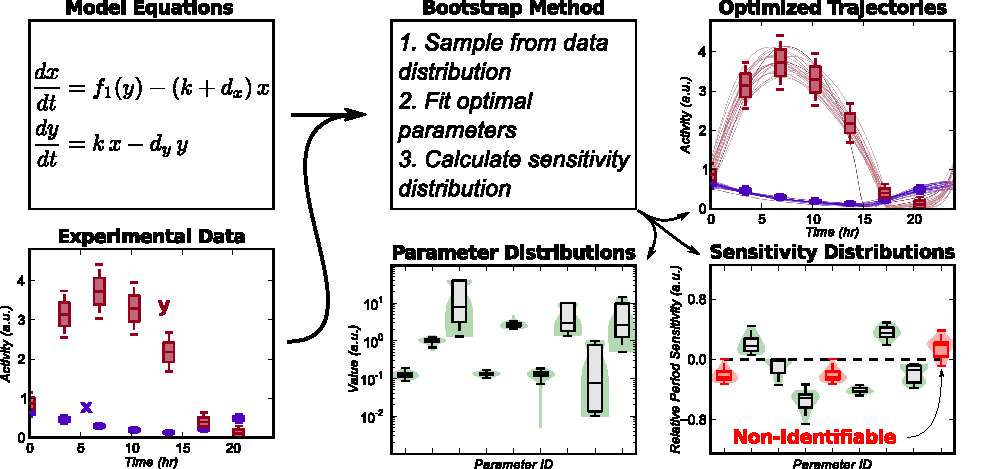
\includegraphics{chap3/figures/fig1.pdf}
  \titlecaption{Parameter estimation and bootstrap methods flowchart}{The demonstrated method calculates confidence intervals in the sensitivity of limit cycle models. An oscillatory model and experimental (or simulated) data are inputs to the bootstrap method. Unique data sets are then used to calculate optimum limit cycle trajectories. The resulting distribution in sensitivities highlight whether a particular response is identifiable (i.e., consistent across the majority of bootstrap trials.)}
  \label{fig:3_1}
\end{figure}

\subsection{Effect of data quality on predictive confidence}

We first analyze the degree to which uncertainty in input data is propagated to uncertainty in output predictions. 
To achieve this, we generate {\itshape in silico} data from a previously published model of circadian rhythms (\fref{mod:hirota}), using relative error $\xi$ to generate normally distributed data ($\sigma_{ij} = \xi \; \hat{x}_{i}(t_j)$) at each of $\cal M$ sampling points. 
As expected, solution trajectories drifted further from the nominal limit cycle for higher values of error, $\xi$, or lower sampling density, $\cal M$, (\fref{fig:3_2}). 
However, the overall shape of the oscillatory profiles remained relatively similar, even for rather high $\xi$ or low $\cal M$.

\begin{figure}[p]
  \centering
  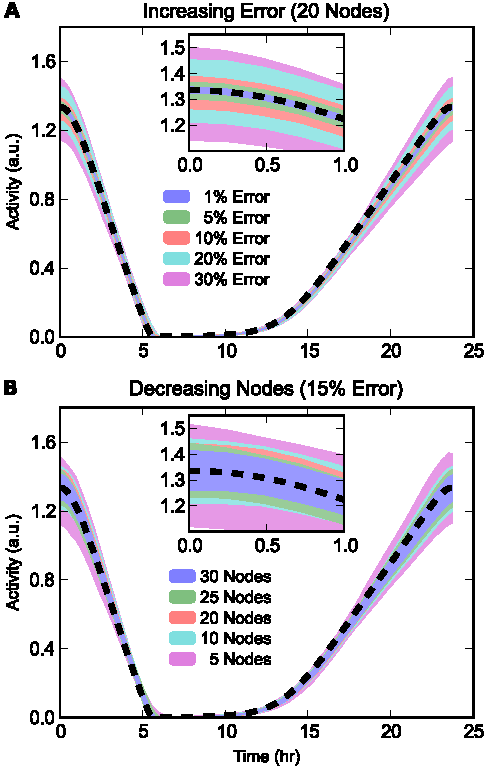
\includegraphics{chap3/figures/fig2.pdf}
  \titlecaption{Time-course profiles of the state trajectories for {\itshape Per mRNA}}{({\bfseries A}) Increasing relative error, $\xi$, with ${\cal M} = 20$. Possible state variable values are shown as shaded regions, obtained by filling between the 5$^\text{th}$ and 95$^\text{th}$ percentile for values at each time for 2000 independent parameter estimations. Increasing $\xi$ results in larger deviations from the original model trajectory, shown as a dashed black line.\\ ({\bfseries B}) Decreasing number of measurement points, $\cal M$, each with $\xi = 0.15$.  Higher $\cal M$ results in trajectories closer to the true trajectory.}
  \label{fig:3_2}
\end{figure}

\Fref{fig:3_3} shows violin plots of the probability distribution for each parameter set and corresponding sensitivity evaluation for increasing $\xi$, while \fref{fig:3_4} shows similar plots for decreasing $\cal M$. 
Interestingly, there is little correlation between the identifiability of a parameter and its corresponding sensitivity value. 
For example, vdP, the maximum degradation rate of Per mRNA, shows a very tight clustering about its nominal parameter value, while the sensitivity of this parameter loses identifiability for even small values of $\xi$. 
Conversely, KdCn, the Michealis-Menten constant associated with the degradation of nuclear CRY, shows large variations in possible parameter values. 
However, the period sensitivity of KdCn, despite lying close to the x-axis, remains identifiable, indicating a robust prediction. 
These results reveal which model responses are constrained by the structure and dynamics of the limit cycle oscillations, and which are dependent on the particular parameterization chosen.

\begin{figure}[p]
  \centering
  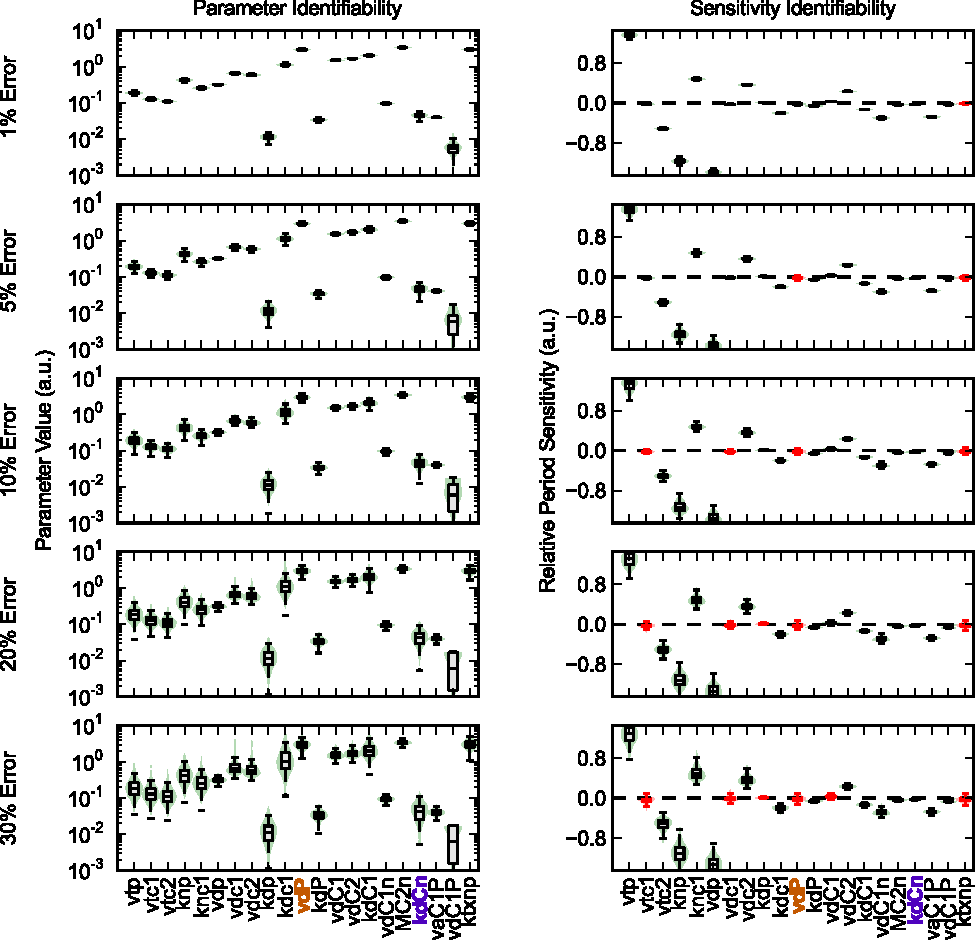
\includegraphics{chap3/figures/fig3.pdf}
  \titlecaption{Parameter and sensitivity identifiability for increasing error}{Increasing $\xi$ results in a corresponding decrease in the confidence of the parameter and sensitivity estimates. Violin plots of the parameter values (left) and relative period sensitivities (right) show the distribution of values from each parameter estimation. In the plots, a box plot is superimposed above a kernel density plot to convey the distribution of values. The whiskers used extend to the most extreme data point within 1.5x the inner quartile range. Sensitivities in which the 5$^\text{th}$ and 95$^\text{th}$ percentile values span the x-axis are deemed non-identifiable (red), as the model's response direction can not be accurately estimated.  Higher $\xi$ also results in wider parameter distributions.}
  \label{fig:3_3}
\end{figure}

\begin{figure}[p]
  \centering
  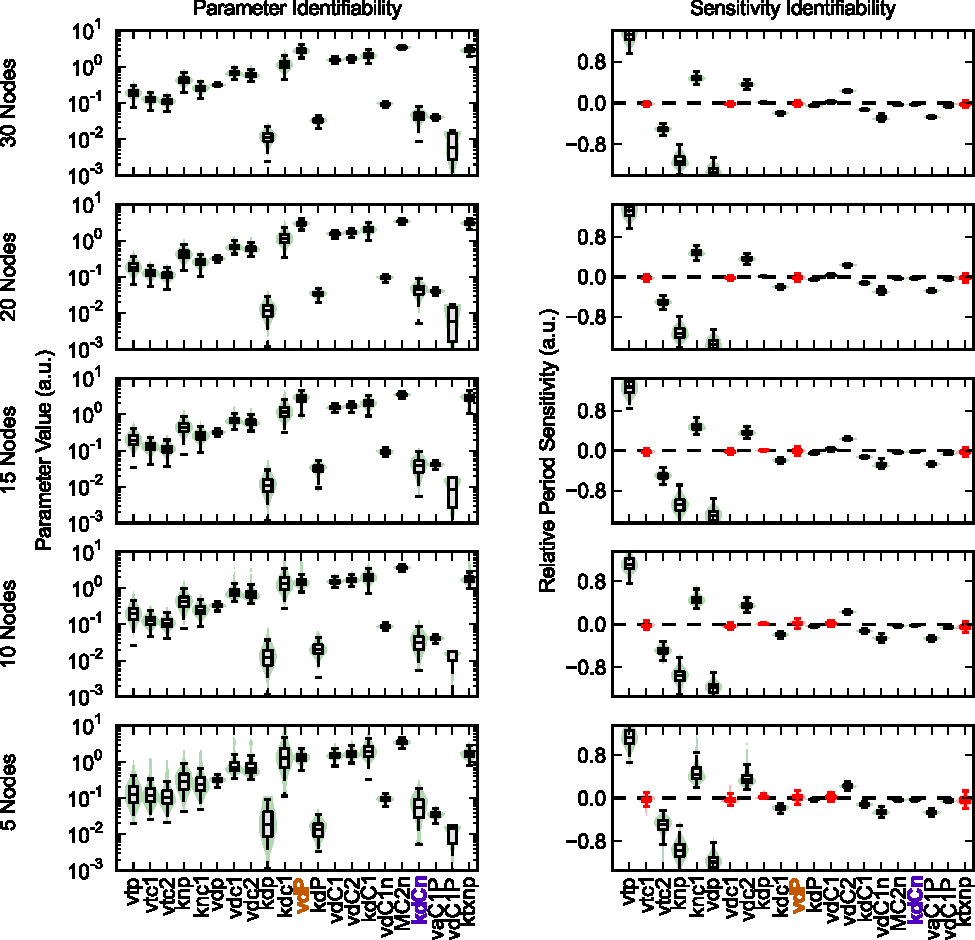
\includegraphics{chap3/figures/fig4.pdf}
  \titlecaption{Effect of high-resolution sampling on identifiability}{ Lower values of $\cal M$ result in less constrained parameter and sensitivity values. Similar to \fref{fig:3_3}, violin plots of the parameters (left) and sensitivities (right) show the distribution from each parameter estimation for decreasing $\cal M$. These results highlight the importance of high-resolution time sampling in generating sensitivity information for oscillatory models.}
  \label{fig:3_4}
\end{figure}

Sensitivities that are experimentally distinguishable from zero are the most important for validation. 
Calculating a typical experimental value for a relative period sensitivity helps to calibrate which sensitivities might be verified experimentally. 
Referring to a recent RNA interference screen, periods changes of approximately 1 hour (~5\%) can be reliably measured using luminescence recordings \cite{Zhang2009}. 
Assuming an increase in the corresponding mRNA degradation parameter value of 50\%, this translates to a relative period sensitivity of ~0.1. 
Thus, many of the identifiable values shown in figures \ref{fig:3_3}-\ref{fig:3_4} fall within the experimentally measurable range. 

\subsection{Application to literature data for model discrimination}
We next apply the method to literature time-course data for core clock components \cite{Lee2001}. 
When modeling a genetic regulatory network, many candidate model equations are often considered. 
We show that a bootstrap uncertainty analysis can also be useful in discriminating between potential model structures based on predictive confidence. 
Here two variations of the same model are fit: The first model (\fref{mod:hirota}) was originally optimized using a genetic algorithm approach, and thus contains a minimal number of parameters to reduce optimization complexity. 
The second model (\fref{mod:hirota2}) considered  contains independent parameters for each rate expression, increasing the number of parameters from 23 to 35. 

\begin{model}[h]
  \centering
  \titlecaption{An expanded parameterization of \fref{mod:hirota}}{These equations have similar reaction stoichiometry to those in table \ref{mod:hirota}, but with more parametric degrees of freedom. This model showed better time-series performance than the more constrained model when fit to time-series data.}

  \begin{align*}
    \frac{d\mathrm{\bf p}}{dt} &= \frac{\mathit{Vm}_{1}}{1 + \mathit{Vm}_{1} \; {\left(\frac{\mathrm{\bf C1N} + \mathrm{\bf C2N} \; \mathit{M}_{1}}{\mathit{Ki}_{1}}\right)}^{3}} - \frac{\mathit{k}_{1} \; \mathrm{\bf p}}{1 + \frac{\mathrm{\bf p}}{\mathit{Km}_{1}}} \\
    \frac{d\mathrm{\bf c1}}{dt} &= \frac{\mathit{Vm}_{2}}{1 + \mathit{Vm}_{2} \; {\left(\frac{\mathrm{\bf C1N} + \mathrm{\bf C2N} \; \mathit{M}_{2}}{\mathit{Ki}_{2}}\right)}^{3}} - \frac{\mathit{k}_{2} \; \mathrm{\bf c1}}{1 + \frac{\mathrm{\bf c1}}{\mathit{Km}_{2}}} \\
    \frac{d\mathrm{\bf c2}}{dt} &= \frac{\mathit{Vm}_{3}}{1 + \mathit{Vm}_{3} \; {\left(\frac{\mathrm{\bf C1N} + \mathrm{\bf C2N} \; \mathit{M}_{3}}{\mathit{Ki}_{3}}\right)}^{3}} - \frac{\mathit{k}_{3} \; \mathrm{\bf c2}}{1 + \frac{\mathrm{\bf c2}}{\mathit{Km}_{3}}} \\
    \frac{d\mathrm{\bf P}}{dt} &= \mathit{k}_{4} \; \mathrm{\bf p} + \mathit{k}_{12} \; \mathrm{\bf C1N} + \mathit{k}_{13} \; \mathrm{\bf C2N} - \frac{\mathit{k}_{7} \; \mathrm{\bf P}}{1 + \frac{\mathrm{\bf P}}{\mathit{Km}_{4}}} - \mathit{k}_{10} \; \mathrm{\bf P} \; \mathrm{\bf C1} - \mathit{k}_{11} \; \mathrm{\bf P} \; \mathrm{\bf C2} \\
    \frac{d\mathrm{\bf C1}}{dt} &= \mathit{k}_{5} \; \mathrm{\bf c1} + \mathit{k}_{12} \; \mathrm{\bf C1N} - \frac{\mathit{k}_{8} \; \mathrm{\bf C1}}{1 + \frac{\mathrm{\bf C1}}{\mathit{Km}_{5}}} - \mathit{k}_{10} \; \mathrm{\bf P} \; \mathrm{\bf C1} \\
    \frac{d\mathrm{\bf C2}}{dt} &= \mathit{k}_{6} \; \mathrm{\bf c2} + \mathit{k}_{13} \; \mathrm{\bf C2N} - \frac{\mathit{k}_{9} \; \mathrm{\bf C2}}{1 + \frac{\mathrm{\bf C2}}{\mathit{Km}_{6}}} - \mathit{k}_{11} \; \mathrm{\bf P} \; \mathrm{\bf C2} \\
    \frac{d\mathrm{\bf C1N}}{dt} &= \mathit{k}_{10} \; \mathrm{\bf P} \; \mathrm{\bf C1} - \mathit{k}_{12} \; \mathrm{\bf C1N} - \frac{\mathit{k}_{14} \; \mathrm{\bf C1N}}{1 + \frac{\mathrm{\bf C1N} + \mathrm{\bf C2N} \; \mathit{M}_{4}}{\mathit{Km}_{7}}} \\
    \frac{d\mathrm{\bf C2N}}{dt} &= \mathit{k}_{11} \; \mathrm{\bf P} \; \mathrm{\bf C2} - \mathit{k}_{13} \; \mathrm{\bf C2N} - \frac{\mathit{k}_{15} \; \mathrm{\bf C2N}}{1 + \frac{\mathrm{\bf C1N} + \mathrm{\bf C2N} \; \mathit{M}_{5}}{\mathit{Km}_{8}}} 
  \end{align*}
  \label{mod:hirota2}
\end{model}


\begin{table}[p]
  \titlecaption{Parameter values for \fref{mod:hirota2}}{Parameters were fit to time-series data via nonlinear programming.}
  \label{tab:parsetopt}
  \vspace{2mm}
  \centering
  \begin{tabular}{cllr} \toprule
           & Parameter        & Description                      & Value  \\ \midrule
    1      & $\mathit{M}_{1}$  & {\itshape Per}/CRY2 activity coefficient    & \num{3.632e+00} \\
    2      & $\mathit{Vm}_{1}$ & {\itshape Per} transcription rate           & \num{9.957e-01} \\
    3      & $\mathit{Ki}_{1}$ & {\itshape Per}/CRY inhibition coefficient   & \num{1.054e-01} \\
    4      & $\mathit{M}_{2}$  & {\itshape Cry1}/CRY2 activity coefficient   & \num{1.000e-03} \\
    5      & $\mathit{Vm}_{2}$ & {\itshape Cry1} transcription rate          & \num{2.262e-01} \\
    6      & $\mathit{Ki}_{2}$ & {\itshape Cry1}/CRY inhibition coefficient  & \num{2.049e-01} \\
    7      & $\mathit{M}_{3}$  & {\itshape Cry2}/CRY2 activity coefficient   & \num{1.000e+01} \\
    8      & $\mathit{Vm}_{3}$ & {\itshape Cry2} transcription rate          & \num{1.850e-01} \\
    9      & $\mathit{Ki}_{3}$ & {\itshape Cry2}/CRY inhibition coefficient  & \num{1.427e-01} \\
    10     & $\mathit{k}_{1}$  & {\itshape Per} degradation rate             & \num{2.920e-01} \\
    11     & $\mathit{Km}_{1}$ & {\itshape Per} degradation self-inhibition  & \num{6.609e-01} \\
    12     & $\mathit{k}_{2}$  & {\itshape Cry1} degradation rate            & \num{1.000e+01} \\
    13     & $\mathit{Km}_{2}$ & {\itshape Cry1} degradation self-inhibition & \num{1.823e-02} \\
    14     & $\mathit{k}_{3}$  & {\itshape Cry2} degradation rate            & \num{4.711e-02} \\
    15     & $\mathit{Km}_{3}$ & {\itshape Cry2} degradation self-inhibition & \num{1.000e+01} \\
    16     & $\mathit{k}_{4}$  & {\itshape Per} translation rate             & \num{1.132e-01} \\
    17     & $\mathit{k}_{5}$  & {\itshape Cry1} translation rate            & \num{3.409e-01} \\
    18     & $\mathit{k}_{6}$  & {\itshape Cry2} translation rate            & \num{1.961e-01} \\
    19     & $\mathit{k}_{7}$  & PER degradation rate             & \num{1.000e+01} \\
    20     & $\mathit{Km}_{4}$ & PER degradation self-inhibition  & \num{1.911e-03} \\
    21     & $\mathit{k}_{8}$  & CRY1 degradation rate            & \num{1.000e+01} \\
    22     & $\mathit{Km}_{5}$ & CRY1 degradation self-inhibition & \num{2.077e-02} \\
    23     & $\mathit{k}_{9}$  & CRY2 degradation rate            & \num{1.000e+01} \\
    24     & $\mathit{Km}_{6}$ & CRY2 degradation self-inhibition & \num{1.180e-02} \\
    25     & $\mathit{k}_{10}$ & C1N association rate             & \num{5.022e-01} \\
    26     & $\mathit{k}_{11}$ & C2N association rate             & \num{1.035e+00} \\
    27     & $\mathit{k}_{12}$ & C1N dissociation rate            & \num{1.000e-03} \\
    28     & $\mathit{k}_{13}$ & C2N dissociation rate            & \num{2.070e-01} \\
    29     & $\mathit{M}_{4}$  & CRY1n/CRY2n activity coefficient & \num{1.000e+01} \\
    30     & $\mathit{k}_{14}$ & CRY1N degradation rate           & \num{1.000e+01} \\
    31     & $\mathit{Km}_{7}$ & CRY1n degradation inhibition     & \num{5.206e-03} \\
    32     & $\mathit{M}_{5}$  & CRY2n/CRY2n activity coefficient & \num{1.000e+01} \\
    33     & $\mathit{k}_{15}$ & CRY2n degradation rate           & \num{1.000e+01} \\
    34     & $\mathit{Km}_{8}$ & CRY2n degradation inhibition     & \num{1.829e-02} \\ \bottomrule
    \hline
  \end{tabular}
\end{table}

\begin{figure}[p]
  \centering
  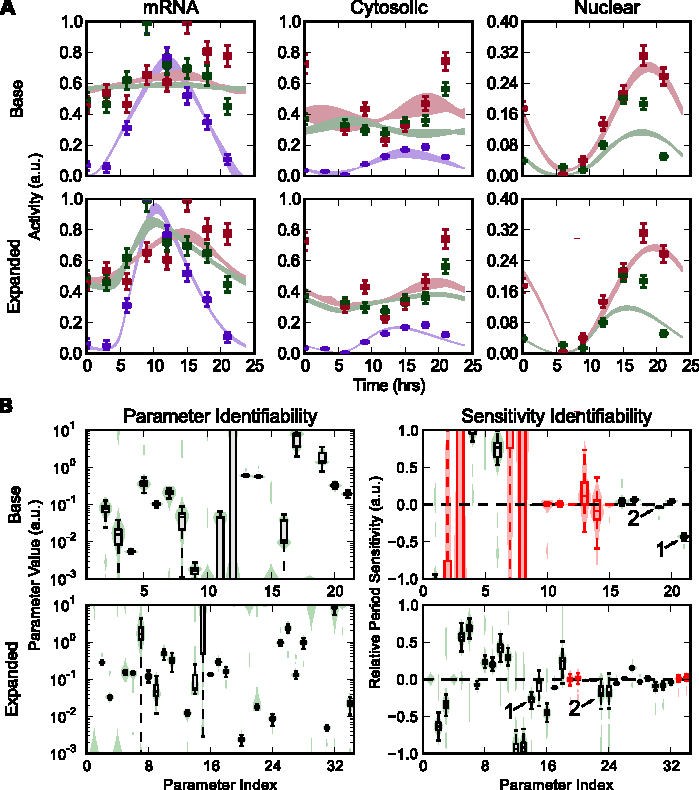
\includegraphics{chap3/figures/fig5.pdf}
  \titlecaption{Identifiability comparison of two model structures}{ ({\bfseries A}) Bootstrap parameter estimations on two model structures using literature time-series data with estimated errors (box plots). Resulting regions of model trajectories are shaded between the 5$^\text{th}$ and 95$^\text{th}$ percentile.  {\itshape Per} species are shown in purple, {\itshape Cry1} in red, and {\itshape Cry2} in green. While both models were able to approximately reproduce the same dynamic response, the expanded model was better able to capture differences between the {\itshape Cry1} and {\itshape Cry2} profiles. ({\bfseries B}) Parameter and sensitivity identifiability for the base and expanded models.  Violin plots show the parameter and sensitivity distributions, with unidentifiable sensitivities (90\% confidence level) highlighted in red.  Despite containing more parameters, the expanded model shows better parameter identifiability and higher confidence in its predicted sensitivities. The PER translation rate (1) and PER-CRY association rate (2) sensitivities are consistent across model equations and are highlighted.}
  \label{fig:3_5}
\end{figure}

The literature data used consisted of 7-8 concentration time points across a 24 hour period. 
Confidence intervals in the data were not available, so an optimistic 3\% relative and 0.5\% absolute error was assumed for each data point ($\sigma_{ij} = 0.03\;\hat{x}_{i}(t_j) + 0.005\;\max(\hat{x}_i)$). 
\Fref{fig:3_5}A shows the resulting time-series profiles for bootstrap estimations of each model. 
While additional kinetic parameters are typically thought to lower the predictive confidence of a model (the `curse of dimensionality'), the expanded model is able to better capture the oscillatory profiles with lower variability between solutions. 
Parameter and sensitivity distributions, figure \ref{fig:3_5}B, similarly show how the expanded model parameterization is able to generate more confident predictions in model response. 
Since the resulting sensitivity identifiability for both models was relatively poor, we highlight sensitivities which pass a 90\% confidence level threshold. 
These results thus indicate higher-resolution data on circadian components would help in conferring confidence to model predictions.

Two sensitivities, the PER translation rate (figure \ref{fig:3_5}B, 1) and the PER-CRY association rate (2), had high confidence and consistent direction in both the base and expanded parameterization - suggesting that the predicted values are robust to slight changes in both parameter value and model structure. 
Since a biological system can be modeled using many different combinations of kinetic assumptions, such a technique will likely prove useful in finding consistent predictions which are robust to slight differences in model equations.

\Fref{fig:3_6} compares optimal fits for both the base and expanded models to the originally published parameter set \cite{Hirota2012}. 
Since the original cost function was concerned mostly with optimizing stoichiometric and knockout data, the refitted models are able to much more accurately represent the time-series dynamics. 

\begin{figure}[p]
  \centering
  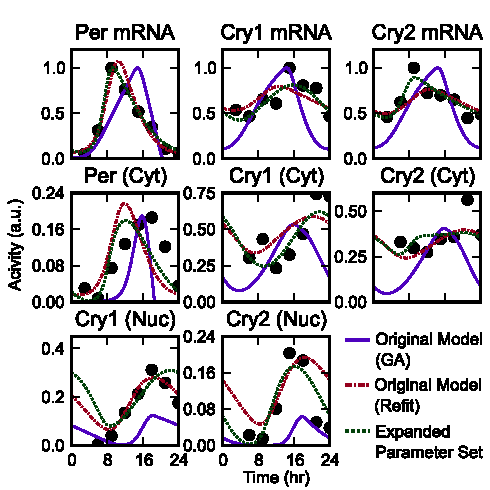
\includegraphics{chap3/figures/fig6.pdf}
  \titlecaption{Time-series dynamics of fitted models}{Model trajectories for each of the considered models. The original model (purple) shows the time series dynamics for the previously published parameter set, used in Figures 1-4. In these plots, the original model's period and amplitudes were rescaled to best match the experimental data, shown in black (without changing the dynamic profiles). The refitted model (red, dashed) was generated by optimizing the dynamic profile to time series data using the parameter estimation routine described in Supplemental Text 1. The expanded model (green, dashed) consists of a similar network structure, but with independent kinetic parameters for each rate expression (see Supplemental Text 2). These plots show that parameter optimization through nonlinear programming is able to more accurately fit gene and protein expression profiles.}
  \label{fig:3_6}
\end{figure}

\section{Discussion}
Increasingly, mathematical models are being used to study biological systems where traditional experiments would prove infeasible. 
 For example, in the search for drug targets, thousands of possible combinatorial perturbations can be quickly scanned for therapeutic effects using {\itshape in silico} modeling. 
This is especially useful in oscillatory systems with long periods, such as circadian rhythms, where a perturbed {\itshape in vitro} or {\itshape in vivo} system must be measured for multiple days before changes can be reliably determined.
 
However, since errors in model responses can arise from either incorrect structure or measurement noise, our confidence in {\itshape in silico} predictions is limited. 
Here we have developed a bootstrap approach suitable for periodic systems, and extended it to include uncertainty in predicted responses. 
With this method, errors due to local parameter effects can be identified, even in models with complicated dynamics. 
Furthermore, by considering multiple variations in model assumptions, we have demonstrated that more trustworthy model predictions can be found.

Since this method takes advantage of time-series data to generate a strong initial guess for an otherwise difficult parameter estimation, it requires high-resolution data on the concentrations of all species in the model. 
In many biological systems, such data is only available for the activity levels of certain well-studied species. 
However, the continued development of high-throughput genomic and proteomic techniques promise to deliver time-series data for a much larger network of components. 
With expanding datasets, these methods will likely prove useful for the quantitative evaluation of uncertainty in larger biological models.

In the following chapter, we apply this method to several existing circadian models in order find conserved predictions across different model kinetics and parameterizations. 
Such an approach allows us to further differentiate between the actions of two seemingly similar small molecule perturbations. 

\chapter[Spatiotemporal separation of PER and CRY posttranslational regulation]{Spatiotemporal separation of PER and CRY posttranslational regulation\footnote{Portions of this chapter are published in P. C. St. John, T. Hirota, S. A. Kay, and F. J. Doyle, ``Spatiotemporal separation of PER and CRY posttranslational regulation in the mammalian circadian clock.,'' {\itshape Proc. Natl. Acad. Sci. U. S. A.}, vol. 111, pp. 2040–5, Feb. 2014.}}

In the previous chapter, computationally efficient techniques for preforming a bootstrap analysis on circadian models was described. 
In this chapter, we apply this technique to clarify the roles of two posttranslational regulators in the core circadian feedback loop. 
Since direct experimental evidence of the systems-level effect of these regulators is difficult if not impossible to obtain, we must rely on computational modeling to provide insight into the dynamic consequences of modulating posttranslational activity. 
For this reason, bootstrap methods are invaluable in generating confident {\itshape in silico} results. 

\section{Background}

Since circadian and metabolic regulators are tightly integrated, circadian disruptions often manifest in metabolic disease \cite{Bass2012}. 
Recent efforts have therefore sought to gain a mechanistic understanding of these pathways, such that the metabolic burdens imposed by a 24-hour society might be mitigated. 
Posttranslational regulators, which play key roles in connecting circadian and metabolic processes, serve as likely targets for future therapeutics -- demonstrated by the wealth of available circadian-active small molecules \cite{Chen2013}.

\subsection{Nuclear entry of PER-CRY complex}
% Oscillations in circadian gene transcription are generated through a time-delayed transcription-translation negative-feedback loop. 
% In mammals, transcription factors CLOCK and BMAL1 promote transcription of E box-containing genes {\it Period} ({\it Per}) and {\it Cryptochrome} ({\it Cry}) (\fref{fig:4-1a}). 
% PER and CRY protein products form heterodimers to accumulate in the nucleus, in which PER is stoichiometrically limiting \cite{Lee2001}, and subsequently close the negative feedback loop by inhibiting CLOCK-BMAL1-promoted gene expression. 
% While steady-state endpoint assays have shown the possibility of nuclear entry of CRY without PER \cite{Ye2011, Kume1999, Yagita2002}, experiments from {\it Per1}\textsuperscript{-/-} {\it Per2}\textsuperscript{-/-} mice demonstrated that PER proteins are required for the timely nuclear accumulation of CRY \cite{Lee2001}. 
% Clearance of nuclear repressors reactivates CLOCK-BMAL1, allowing the cycle to begin anew \cite{Takahashi2008}. 

Experimental evidence on PER/CRY nuclear entry is seemingly contradictory. 
For nuclear localization of the PER and CRY proteins, experiments from {\it Per1}\textsuperscript{-/-} {\it Per2}\textsuperscript{-/-} mice demonstrate that PER proteins are required for timely nuclear accumulation of CRY \cite{Lee2001}. 
While other studies have shown the possibility of nuclear entry of CRY without PER, these results are typically based on steady-state endpoint assays which do not consider the speed of CRY nuclear entry \cite{Ye2011, Kume1999, Yagita2002}. 
We therefore consider the formation of the PER-CRY heterodimer as a key step in nuclear entry, which is supported by the fact that to the best of our knowledge all circadian models that consider both PER and CRY employ this kinetic assumption \cite{Hirota2012, Relogio2011, Leloup2003, Forger2003, Mirsky2009}.

\subsection{Importance of posttranslational regulators}
The stabilities of PER and CRY are tightly regulated: PER proteins are phosphorylated by the casein kinase I family of proteins (CKI$\delta/\epsilon$), prompting $\beta$-TrCP-mediated degradation \cite{Reischl2007} and nuclear import \cite{Takano2004}. 
The degradation of CRY proteins is separately regulated by the SCF\textsuperscript{FBXL3} ubiquitin ligase complex \cite{Busino2007, Godinho2007, Siepka2007}. 
The activities of both CKI-PER and FBXL3-CRY may be further coupled to the cell's metabolic state through AMPK signalling \cite{Lee2013}. 
These posttranslational regulatory mechanisms have a strong effect on period length: the gain-of-function mutant CKI$\epsilon^\mathrm{tau}$ leading to hyperphosphorylation of PER \cite{Gallego2006} and small molecule CKI inhibitors, such as longdaysin \cite{Hirota2010}, demonstrated that increasing or decreasing CKI-dependent PER phosphorylation shortens or lengthens the period, respectively. 
In contrast, genetic mutations of FBXL3 \cite{Godinho2007, Siepka2007} and KL001, a small molecule inhibitor of FBXL3-dependent CRY degradation \cite{Hirota2012}, showed that increased CRY stability leads to longer periods. 
Since the scale and complexity of the circadian network complicates an intuitive understanding of these relationships, mathematical models have played important roles in understanding how these manipulations affect circadian period \cite{Gallego2006, Hirota2012, Reischl2007}.

\subsection{Functional differences between PER and CRY}
Given that both CKI and FBXL3 pathways regulate the stability of linked negative factors, it was thought that simultaneous perturbations to both pathways might lead to non-additive effects: i.e., the slowest link would determine the period. 
 However, both small molecule \cite{Hirota2012} and genetic experiments \cite{Maywood2011} have demonstrated the independent period effects of these two posttranslational regulations. 
A recent clarification of the canonical clock feedback circuit has shown that dissociated CRY is the dominant repressor of CLOCK-BMAL1 mediated E box transcription \cite{Ye2011}. 
This distinction helps differentiate between the roles of the otherwise similar PER and CRY proteins, in which the main role of PER in transcriptional repression is likely regulating the timing of nuclear accumulation of CRY. 
Therefore, while previous mathematical models in which PER acts as a direct repressor have proposed mechanisms for CKI-dependent period lengthening \cite{Gallego2006, Vanselow2006}, they are likely not suitable for distinguishing between CKI-PER and FBXL3-CRY mediated period change.

In this chapter, we used human cells harboring clock gene reporters together with mathematical modeling to gain insight into the relationship between PER and CRY posttranslational regulation. 
Consequently, we provide a new mechanism by which CKI-dependent PER phosphorylation controls the circadian period separately from the FBXL3-CRY pathway. 
The resulting detailed understanding of PER and CRY regulation in the core feedback loop provides a framework on which to interpret metabolic and pharmacological control of circadian rhythms.

\section{Methods}
\subsection{Analysis of luminescence profiles}
Raw luminescence data was first separated into a moving baseline and oscillatory component using a Hodrick-Prescott filter with a smoothing parameter of 1600. 
Example trajectory decompositions are shown in \fref{fig:4s1}. 
Amplitudes (as shown in \fref{fig:4-1b}) were determined by taking the standard deviation in the baseline-subtracted data. 
Periods were obtained by nonlinear curve fitting, in which a four parameter (initial amplitude, decay, period and phase) damped cosine curve was fit to the baseline-subtracted data. 
Periods were not shown if the relative amplitude (found by standard deviation) fell below 25\%, since noise dominated the periodic trajectory. 

\begin{figure}[p]
  \centering
  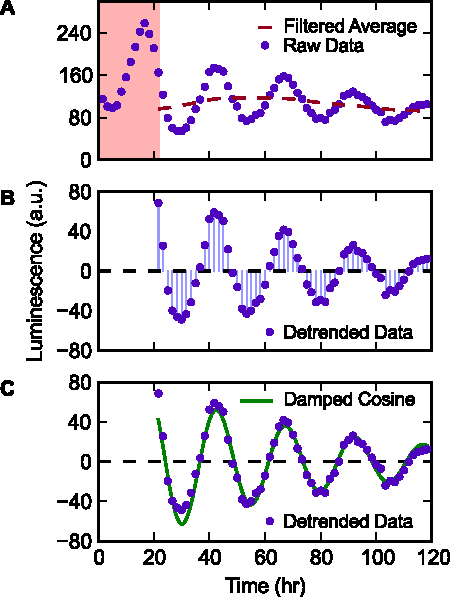
\includegraphics[width=0.6\textwidth]{chap4/figures/figS1.pdf}
  \titlecaption{Analysis of circadian reporter luminescence data}{ ({\bfseries A}) Raw luminescence data is first cropped by removing the initial transient region (first 12 points). The moving baseline is estimated using a Hodrick-Prescott filter with smoothing parameter 1600 (red dashed line). ({\bfseries B}) Data is detrended by subtracting the moving baseline from the raw data. The detrended data is used to calculate the relative amplitude of the oscillations via standard deviation. ({\bfseries C}) Periods are estimated by fitting a damped cosine curve (green solid line) to the detrended data.}
  \label{fig:4s1}
\end{figure}

\subsection{Cost function}
Models were fit to a cost function of experimental results. 
{\it Per}, {\it Cry}, {\it Clock}, and {\it Bmal1} protein and mRNA levels were taken from \cite{Lee2001}, along with profiles of CRY nuclear localization. 
For the model from \cite{Relogio2011}, additional activity profiles on {\it Rev-Erb} and {\it Ror} were obtained from CircaDB (\url{http://bioinf.itmat.upenn.edu/circa/}). 
To score a model trajectory, mRNA state variables were scaled independently to minimize the squared error between model and experiment, since model parameters could be adjusted to give mRNA profiles arbitrary amplitudes. 
For protein species, where stoichiometric interactions are important, a single scaling parameter was used for all species. 
Nuclear repressor species, in which only relative measurements were available, were scaled independently. 
Full model equations for the model from Hirota {\itshape et al.}, 2012 are shown in \fref{mod:hirota}, the model from Rel\'{o}gio {\itshape et al.} 2011 in \fref{mod:relogioeqs}, and the model from Leloup \& Goldbeter, 2003 in \fref{mod:leloupeqs}.

\begin{model}[p]
  \centering
  \titlecaption{Model from Rel\'{o}gio {\itshape et al.} 2011 \cite{Relogio2011}}{}
  \label{mod:relogioeqs}
  \fontsize{9}{11}

  \begin{align*}
    \frac{d\,\mathit{CLKBM1}}{dt} &= \mathit{BM1n} \cdot \mathit{kfCLKBM1} - \mathit{CLKBM1} \cdot \mathit{dCLKBM1} - \mathit{CLKBM1} \cdot \mathit{kdCLKBM1}\\
    \frac{d\,\mathit{reverb}}{dt} &= \frac{\mathit{V3max} \left(\mathit{g} \cdot
    {\frac{\mathit{CLKBM1}}{\mathit{kt3}}}^{\mathit{v}} +
  1\right)}{{\frac{\mathit{CLKBM1}}{\mathit{kt3}}}^{\mathit{v}}
  {\left(\frac{\mathit{PnCn} + \mathit{PnpCn}}{\mathit{ki3}}\right)}^{\mathit{w}} +
  {\frac{\mathit{CLKBM1}}{\mathit{kt3}}}^{\mathit{v}} + 1} - \mathit{dreverb}
  \cdot \mathit{reverb}\\
  \frac{d\,\mathit{ror}}{dt} &= \frac{\mathit{V4max} \left(\mathit{h} \cdot {\frac{\mathit{CLKBM1}}{\mathit{kt4}}}^{\mathit{p}} + 1\right)}{{\frac{\mathit{CLKBM1}}{\mathit{kt4}}}^{\mathit{p}} \cdot {(\frac{\mathit{PnCn} + \mathit{PnpCn}}{\mathit{ki4}})}^{\mathit{q}} + {\frac{\mathit{CLKBM1}}{\mathit{kt4}}}^{\mathit{p}} + 1} - \mathit{dror} \cdot \mathit{ror}\\
  \frac{d\,\mathit{REVERBc}}{dt} &= - \mathit{REVERBc} \cdot \mathit{dREVERBc} - \mathit{REVERBc} \cdot \mathit{kiREVERBc} + \mathit{kp3} \cdot \mathit{reverb}\\
  \frac{d\,\mathit{RORc}}{dt} &= - \mathit{RORc} \cdot \mathit{dRORc} - \mathit{RORc} \cdot \mathit{kiRORc} + \mathit{kp4} \cdot \mathit{ror}\\
  \frac{d\,\mathit{REVERBn}}{dt} &= \mathit{REVERBc} \cdot \mathit{kiREVERBc} - \mathit{REVERBn} \cdot \mathit{dREVERBn}\\
  \frac{d\,\mathit{RORn}}{dt} &= \mathit{RORc} \cdot \mathit{kiRORc} - \mathit{RORn} \cdot \mathit{dRORn}\\
  \frac{d\,\mathit{bm1}}{dt} &= \frac{\mathit{V5max} \left(\mathit{i} \cdot {\frac{\mathit{RORn}}{\mathit{kt5}}}^{\mathit{n}} + 1\right)}{{\frac{\mathit{REVERBn}}{\mathit{ki5}}}^{\mathit{m}} + {\frac{\mathit{RORn}}{\mathit{kt5}}}^{\mathit{n}} + 1} - \mathit{bm1} \cdot \mathit{dbm1}\\
  \frac{d\,\mathit{BM1c}}{dt} &= - \mathit{BM1c} \cdot \mathit{dBM1c} - \mathit{BM1c} \cdot \mathit{kiBM1c} + \mathit{bm1} \cdot \mathit{kp5}\\
  \frac{d\,\mathit{BM1n}}{dt} &= \mathit{BM1c} \cdot \mathit{kiBM1c} - \mathit{BM1n} \cdot \mathit{dBM1n} - \mathit{BM1n} \cdot \mathit{kfCLKBM1} + \mathit{CLKBM1} \cdot \mathit{kdCLKBM1}\\
  \frac{d\,\mathit{per}}{dt} &= \frac{\mathit{V1max} \left(\mathit{a} \cdot {\frac{\mathit{CLKBM1}}{\mathit{kt1}}}^{\mathit{b}} + 1\right)}{{\frac{\mathit{CLKBM1}}{\mathit{kt1}}}^{\mathit{b}} \cdot {(\frac{\mathit{PnCn} + \mathit{PnpCn}}{\mathit{ki1}})}^{\mathit{c}} + {\frac{\mathit{CLKBM1}}{\mathit{kt1}}}^{\mathit{b}} + 1} - \mathit{dper} \cdot \mathit{per}\\
  \frac{d\,\mathit{cry}}{dt} &= \frac{\mathit{V2max}
  \left(\frac{\mathit{CLKBM1}^{3} \cdot \mathit{d}}{\mathit{kt2}^{3}} +
1\right)}{\left({\frac{\mathit{REVERBn}}{\mathit{ki21}}}^{\mathit{f1}} +
1\right) \left(\frac{\mathit{CLKBM1}^{3}}{\mathit{kt2}^{3}} +
{\frac{\mathit{CLKBM1}}{\mathit{kt2}}}^{\mathit{e}}
{\left(\frac{\mathit{PnCn} +
\mathit{PnpCn}}{\mathit{ki2}}\right)}^{\mathit{f}} + 1\right)} - \mathit{cry}
\cdot \mathit{dcry}\\
\frac{d\,\mathit{Cc}}{dt} &= - \mathit{Cc} \cdot \mathit{Pc} \cdot \mathit{kfPcCc} - \mathit{Cc} \cdot \mathit{Pcp} \cdot \mathit{kfPcpCc} - \mathit{Cc} \cdot \mathit{dCc} + \mathit{PcCc} \cdot \mathit{kdPcCc} + \mathit{PcpCc} \cdot \mathit{kdPcpCc} + \mathit{cry} \cdot \mathit{kp2}\\
\frac{d\,\mathit{Pc}}{dt} &= - \mathit{Cc} \cdot \mathit{Pc} \cdot \mathit{kfPcCc} - \mathit{Pc} \cdot \mathit{dPc} - \mathit{Pc} \cdot \mathit{kphPc} + \mathit{PcCc} \cdot \mathit{kdPcCc} + \mathit{Pcp} \cdot \mathit{kdphPcp} + \mathit{kp1} \cdot \mathit{per}\\
\frac{d\,\mathit{Pcp}}{dt} &= - \mathit{Cc} \cdot \mathit{Pcp} \cdot \mathit{kfPcpCc} + \mathit{Pc} \cdot \mathit{kphPc} - \mathit{Pcp} \cdot \mathit{dPcp} - \mathit{Pcp} \cdot \mathit{kdphPcp} + \mathit{PcpCc} \cdot \mathit{kdPcpCc}\\
\frac{d\,\mathit{PcpCc}}{dt} &= \mathit{Cc} \cdot \mathit{Pcp} \cdot \mathit{kfPcpCc} - \mathit{PcpCc} \cdot \mathit{dPcpCc} - \mathit{PcpCc} \cdot \mathit{kdPcpCc} - \mathit{PcpCc} \cdot \mathit{kiPcpCc} + \mathit{PnpCn} \cdot \mathit{kePnpCn}\\
\frac{d\,\mathit{PcCc}}{dt} &= \mathit{Cc} \cdot \mathit{Pc} \cdot \mathit{kfPcCc} - \mathit{PcCc} \cdot \mathit{dPcCc} - \mathit{PcCc} \cdot \mathit{kdPcCc} - \mathit{PcCc} \cdot \mathit{kiPcCc} + \mathit{PnCn} \cdot \mathit{kePnCn}\\
\frac{d\,\mathit{PnpCn}}{dt} &= \mathit{PcpCc} \cdot \mathit{kiPcpCc} - \mathit{PnpCn} \cdot \mathit{dPnpCn} - \mathit{PnpCn} \cdot \mathit{kePnpCn}\\
\frac{d\,\mathit{PnCn}}{dt} &= \mathit{PcCc} \cdot \mathit{kiPcCc} - \mathit{PnCn} \cdot \mathit{dPnCn} - \mathit{PnCn} \cdot \mathit{kePnCn}\\
\end{align*}
\end{model}

\begin{model}[p]
  \centering
  \titlecaption{Model from Leloup \& Goldbeter, 2003 \cite{Leloup2003}}{}
  \label{mod:leloupeqs}
  \footnotesize

  \begin{align*}
    \frac{d\,\mathit{MP}}{dt} &= - \mathit{MP} \cdot \mathit{kdmp} - \frac{\mathit{MP} \cdot \mathit{vmP}}{\mathit{KmP} + \mathit{MP}} + \frac{\mathit{vsP} \cdot {\mathit{BN}}^{\mathit{n}}}{{\mathit{BN}}^{\mathit{n}} + {\mathit{KAP}}^{\mathit{n}}}\\
    \frac{d\,\mathit{MC}}{dt} &= - \mathit{MC} \cdot \mathit{kdmc} - \frac{\mathit{MC} \cdot \mathit{vmC}}{\mathit{KmC} + \mathit{MC}} + \frac{\mathit{vsC} \cdot {\mathit{BN}}^{\mathit{n}}}{{\mathit{BN}}^{\mathit{n}} + {\mathit{KAC}}^{\mathit{n}}}\\
    \frac{d\,\mathit{MB}}{dt} &= - \mathit{MB} \cdot \mathit{kdmb} - \frac{\mathit{MB} \cdot \mathit{vmB}}{\mathit{KmB} + \mathit{MB}} + \frac{\mathit{vsB} \cdot {\mathit{KIB}}^{\mathit{m}}}{{\mathit{BN}}^{\mathit{m}} + {\mathit{KIB}}^{\mathit{m}}}\\
    \frac{d\,\mathit{PC}}{dt} &= - \mathit{CC} \cdot \mathit{PC} \cdot \mathit{k3} + \mathit{MP} \cdot \mathit{ksP} - \frac{\mathit{PC} \cdot \mathit{V1P}}{\mathit{Kp} + \mathit{PC}} - \mathit{PC} \cdot \mathit{kdn} + \mathit{PCC} \cdot \mathit{k4} + \frac{\mathit{PCP} \cdot \mathit{V2P}}{\mathit{Kdp} + \mathit{PCP}}\\
    \frac{d\,\mathit{CC}}{dt} &= - \mathit{CC} \cdot \mathit{PC} \cdot \mathit{k3} - \frac{\mathit{CC} \cdot \mathit{V1C}}{\mathit{CC} + \mathit{Kp}} - \mathit{CC} \cdot \mathit{kdnc} + \frac{\mathit{CCP} \cdot \mathit{V2C}}{\mathit{CCP} + \mathit{Kdp}} + \mathit{MC} \cdot \mathit{ksC} + \mathit{PCC} \cdot \mathit{k4}\\
    \frac{d\,\mathit{PCP}}{dt} &= \frac{\mathit{PC} \cdot \mathit{V1P}}{\mathit{Kp} + \mathit{PC}} - \frac{\mathit{PCP} \cdot \mathit{V2P}}{\mathit{Kdp} + \mathit{PCP}} - \mathit{PCP} \cdot \mathit{kdn} - \frac{\mathit{PCP} \cdot \mathit{vdPC}}{\mathit{Kdp} + \mathit{PCP}}\\
    \frac{d\,\mathit{CCP}}{dt} &= \frac{\mathit{CC} \cdot \mathit{V1C}}{\mathit{CC} + \mathit{Kp}} - \frac{\mathit{CCP} \cdot \mathit{V2C}}{\mathit{CCP} + \mathit{Kdp}} - \mathit{CCP} \cdot \mathit{kdn} - \frac{\mathit{CCP} \cdot \mathit{vdCC}}{\mathit{CCP} + \mathit{Kd}}\\
    \frac{d\,\mathit{PCC}}{dt} &= \mathit{CC} \cdot \mathit{PC} \cdot \mathit{k3} - \frac{\mathit{PCC} \cdot \mathit{V1PC}}{\mathit{Kp} + \mathit{PCC}} - \mathit{PCC} \cdot \mathit{k1} - \mathit{PCC} \cdot \mathit{k4} - \mathit{PCC} \cdot \mathit{kdn} + \frac{\mathit{PCCP} \cdot \mathit{V2PC}}{\mathit{Kdp} + \mathit{PCCP}} + \mathit{PCN} \cdot \mathit{k2}\\
    \frac{d\,\mathit{PCN}}{dt} &= - \mathit{BN} \cdot \mathit{PCN} \cdot \mathit{k7} + \mathit{IN} \cdot \mathit{k8} + \mathit{PCC} \cdot \mathit{k1} - \frac{\mathit{PCN} \cdot \mathit{V3PC}}{\mathit{Kp} + \mathit{PCN}} - \mathit{PCN} \cdot \mathit{k2} - \mathit{PCN} \cdot \mathit{kdn} + \frac{\mathit{PCNP} \cdot \mathit{V4PC}}{\mathit{Kdp} + \mathit{PCNP}}\\
    \frac{d\,\mathit{PCCP}}{dt} &= \frac{\mathit{PCC} \cdot \mathit{V1PC}}{\mathit{Kp} + \mathit{PCC}} - \frac{\mathit{PCCP} \cdot \mathit{V2PC}}{\mathit{Kdp} + \mathit{PCCP}} - \mathit{PCCP} \cdot \mathit{kdn} - \frac{\mathit{PCCP} \cdot \mathit{vdPCC}}{\mathit{Kd} + \mathit{PCCP}}\\
    \frac{d\,\mathit{PCNP}}{dt} &= \frac{\mathit{PCN} \cdot \mathit{V3PC}}{\mathit{Kp} + \mathit{PCN}} - \frac{\mathit{PCNP} \cdot \mathit{V4PC}}{\mathit{Kdp} + \mathit{PCNP}} - \mathit{PCNP} \cdot \mathit{kdn} - \frac{\mathit{PCNP} \cdot \mathit{vdPCN}}{\mathit{Kd} + \mathit{PCNP}}\\
    \frac{d\,\mathit{BC}}{dt} &= \frac{- \mathit{BC} \cdot \mathit{V1B}}{\mathit{BC} + \mathit{Kp}} - \mathit{BC} \cdot \mathit{k5} - \mathit{BC} \cdot \mathit{kdn} + \frac{\mathit{BCP} \cdot \mathit{V2B}}{\mathit{BCP} + \mathit{Kdp}} + \mathit{BN} \cdot \mathit{k6} + \mathit{MB} \cdot \mathit{ksB}\\
    \frac{d\,\mathit{BCP}}{dt} &= \frac{\mathit{BC} \cdot \mathit{V1B}}{\mathit{BC} + \mathit{Kp}} - \frac{\mathit{BCP} \cdot \mathit{V2B}}{\mathit{BCP} + \mathit{Kdp}} - \mathit{BCP} \cdot \mathit{kdn} - \frac{\mathit{BCP} \cdot \mathit{vdBC}}{\mathit{BCP} + \mathit{Kd}}\\
    \frac{d\,\mathit{BN}}{dt} &= \mathit{BC} \cdot \mathit{k5} - \mathit{BN} \cdot \mathit{PCN} \cdot \mathit{k7} - \frac{\mathit{BN} \cdot \mathit{V3B}}{\mathit{BN} + \mathit{Kp}} - \mathit{BN} \cdot \mathit{k6} - \mathit{BN} \cdot \mathit{kdn} + \frac{\mathit{BNP} \cdot \mathit{V4B}}{\mathit{BNP} + \mathit{Kdp}} + \mathit{IN} \cdot \mathit{k8}\\
    \frac{d\,\mathit{BNP}}{dt} &= \frac{\mathit{BN} \cdot \mathit{V3B}}{\mathit{BN} + \mathit{Kp}} - \frac{\mathit{BNP} \cdot \mathit{V4B}}{\mathit{BNP} + \mathit{Kdp}} - \mathit{BNP} \cdot \mathit{kdn} - \frac{\mathit{BNP} \cdot \mathit{vdBN}}{\mathit{BNP} + \mathit{Kd}}\\
    \frac{d\,\mathit{IN}}{dt} &= \mathit{BN} \cdot \mathit{PCN} \cdot \mathit{k7} - \mathit{IN} \cdot \mathit{k8} - \mathit{IN} \cdot \mathit{kdn} - \frac{\mathit{IN} \cdot \mathit{vdIN}}{\mathit{IN} + \mathit{Kd}}\\
  \end{align*}
\end{model}

\subsection{Parameter estimation and bootstrap analysis}
Bootstrap parameter estimations were performed as described in \fref{chap:id} with data from \cite{Lee2001} assumed to have a normally distributed 10\% relative and 5\% absolute error. 
Since not all states in the models were measured, initial guess values for the trajectory and parameter variables were generated by optimizing the parameter sets first with a genetic algorithm approach, described in \cite{Mirsky2009}. 
To help ensure bootstrap trials remained in a similar stability region of parameter space (and protect against steady-state solutions), bootstrap parameters were bound between 50\% and 150\% of their initial value. 

\subsection{Selection of parameters for FBXL3 and CKI}
For FBXL3-CRY, parameters that determined the degradation rate of CRY (or CRY containing complexes) were considered to be the most likely candidates. 
Michealis-Menten degradation parameters were omitted from \fref{fig:4.3} since perturbations to such parameters are not easily attributable to changes in FBXL3 binding affinity. 
In the model presented in \cite{Leloup2003}, CRY is degraded through a series of phosphorylation events, and these parameters were considered as representative of the rate of progression toward ubiquitination of CRY. 
The forward phosphorylation rates of CRY and nuclear PER-CRY complex were therefore also considered. 
 For CKI-PER, we considered rates that determined the degradation rate and nuclear import rate of PER. 
Michealis-Menten parameters were not included, similar to FBXL3-CRY. 
With CRY being the main repressor of E box transcription \cite{Ye2011}, the degradation rates of PER-CRY complex were not considered as potential mechanisms of CKI. 
In the models of \cite{Leloup2003} and \cite{Relogio2011}, the nuclear entry of PER-CRY requires two independent steps: the formation of the PER-CRY complex and the subsequent import of the complex. 
Therefore, the forward reaction rates of each of these steps were included. 

\subsection{Numerical experiments}
Numerical parameter inhibitions were performed by recalculating the limit cycle trajectory for each new parameter set to a tolerance of $10^{-8}$, using computational methods described previously \cite{Wilkins2009}.

\begin{figure}[tbp]
  \centering
  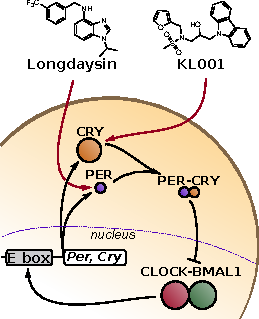
\includegraphics[width=0.4\textwidth]{chap4/figures/fig1_schem.pdf}
  \titlecaption{Small molecule targets}{Schematic of the core circadian feedback loop, with the targets of small molecule modulators longdaysin (CKI inhibitor) and KL001 (inhibitor of FBXL3-dependent CRY degradation) shown. The size of each molecule is representative of relative concentration}
  \label{fig:4-1a}
\end{figure}

\section{Results}

\subsection{Opposite amplitude effects of longdaysin and KL001}
To gain a more detailed understanding of the roles of CKI-PER and FBXL3-CRY pathways, we applied small molecule compounds longdaysin and KL001, which cause stabilization of PER and CRY, respectively \cite{Hirota2010, Hirota2012} (\fref{fig:4-1a}). 
We used {\it Bmal1}- and {\it Per2-dLuc} as circadian reporters, which represent different loops of the core clock mechanism and show circadian luminescence rhythms with mutually opposite phase. 
Time-course data on circadian reporter expression under increasing concentrations of longdaysin and KL001 \cite{Hirota2012} was analyzed for period and amplitude change (\fref{fig:4-1b}).
Longdaysin caused dose-dependent increases in period and detrended amplitude to $\approx 50\%$ of control values in both {\it Bmal1}- and {\it Per2-dLuc} reporter cells. 
In contrast, KL001 induced a simultaneous increase in period and strong reduction in amplitude. 
Modulation of the activity of CKI-PER and FBXL3-CRY is therefore differentiated by an opposite amplitude response.

\begin{figure}[h]
  \centering
  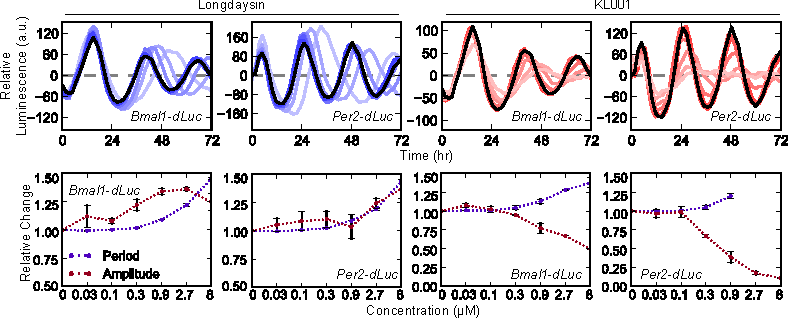
\includegraphics[width=\textwidth]{chap4/figures/fig1_ts.pdf}
  \titlecaption{Different amplitude effect of small molecule circadian modulators targeting CKI-PER and FBXL3-CRY}{(top) Detrended luminescence profiles (first 72 hours, mean of two independent replications) obtained from U2OS reporter cells with increasing concentration of longdaysin and KL001. Black profiles indicate control conditions (0 $\mu$M), lighter colors indicate higher concentrations of small molecule (from 0.03 to 8 $\mu$M). (bottom) Relative change in period and amplitude of the results in shown on top.}
  \label{fig:4-1b}
\end{figure}

\subsection{Main period-determining perturbations}

We next used {\it in silico} modeling to gain mechanistic insight into CKI-PER and FBXL3-CRY mediated circadian regulation. 
In \fref{chap:model}, I described the connection between inhibition of FBXL3-dependent CRY degradation and period change \cite{Hirota2012}: increasing the stability of nuclear CRY results in longer transcriptional repression and increased period length. 
However, while CKI has been linked to modulating PER stability and nuclear entry, it remained unclear which perturbation dominates the period effect, and whether these processes are sufficient to separate the effects of CKI and FBXL3.

To generate predictions that are consistent across slight differences in model assumptions, we chose three mathematical models from the literature based on their moderate size and similar scope \cite{Hirota2012, Leloup2003, Relogio2011}. 
The models included, at a minimum, the expression and nuclear entry mechanisms of PER and CRY. 
We considered the formation of the PER-CRY heterodimer as a key step in nuclear entry, which is supported by the fact that, to the best of our knowledge, all circadian models that consider both PER and CRY employ this kinetic assumption \cite{Hirota2012, Relogio2011, Leloup2003, Forger2003, Mirsky2009}.

Since dynamic models of genetic regulatory networks typically suffer from poor parameter identifiability \cite{Gunawan2006}, we demonstrate that our predictions are parameter-independent by employing a bootstrap identifiability analysis \cite{St.John2013}. 
As part of the bootstrap method, the models were re-fit to experimental data \cite{Lee2001} while ensuring appropriate protein stoichiometry. 
The state trajectories of the resulting 2000 parameter sets for each model are shown in \fref{fig:4.2}, with reasonable agreement between models and experiment.

\begin{figure}[h]
  \centering
  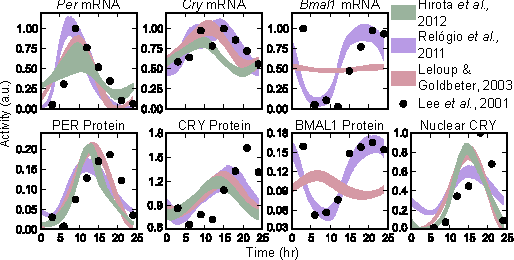
\includegraphics[width=0.8\textwidth]{chap4/figures/fig2.pdf}
  \titlecaption{Fitted trajectories from bootstrap runs}{Time series trajectories of the 2000 bootstrap trials for each model. Shaded regions indicate 95\% confidence regions. The data were scaled to have a maximum value of 1, except for protein species, where relative values were important for clock stoichiometry.}
  \label{fig:4.2}
\end{figure}


A first-order period sensitivity analysis, performed on each of the parameter sets, identified which parameters associated with PER and CRY protein activity had the greatest effect on period (\fref{fig:4.s2}). 
To simplify analysis, we present only those parameters that are associated with experimentally supported mechanisms of CKI and FBXL3 in \fref{fig:4.3}. 
We first tested parameters associated with potential FBXL3-CRY activity to evaluate if our method matched the experimentally verified effect of KL001 \cite{Hirota2012}. 
Since CRY is the dominant repressor of CLOCK-BMAL1 \cite{Ye2011}, we attribute degradation rates of the PER-CRY complex to be representative of CRY clearance rates. 
We found that only parameters governing nuclear CRY degradation show a period lengthening effect upon inhibition, while rates associated with cytoplasmic CRY degradation show period shortening effects. 
These results match with our previous assertion that period lengthening occurs via nuclear CRY stabilization \cite{Hirota2012}. 
Experimental evidence has also indicated cytoplasmic CRY stabilization may lead to period shortening \cite{Kurabayashi2010}, a result consistent with our mathematical results.

\begin{figure}[p]
  \centering
  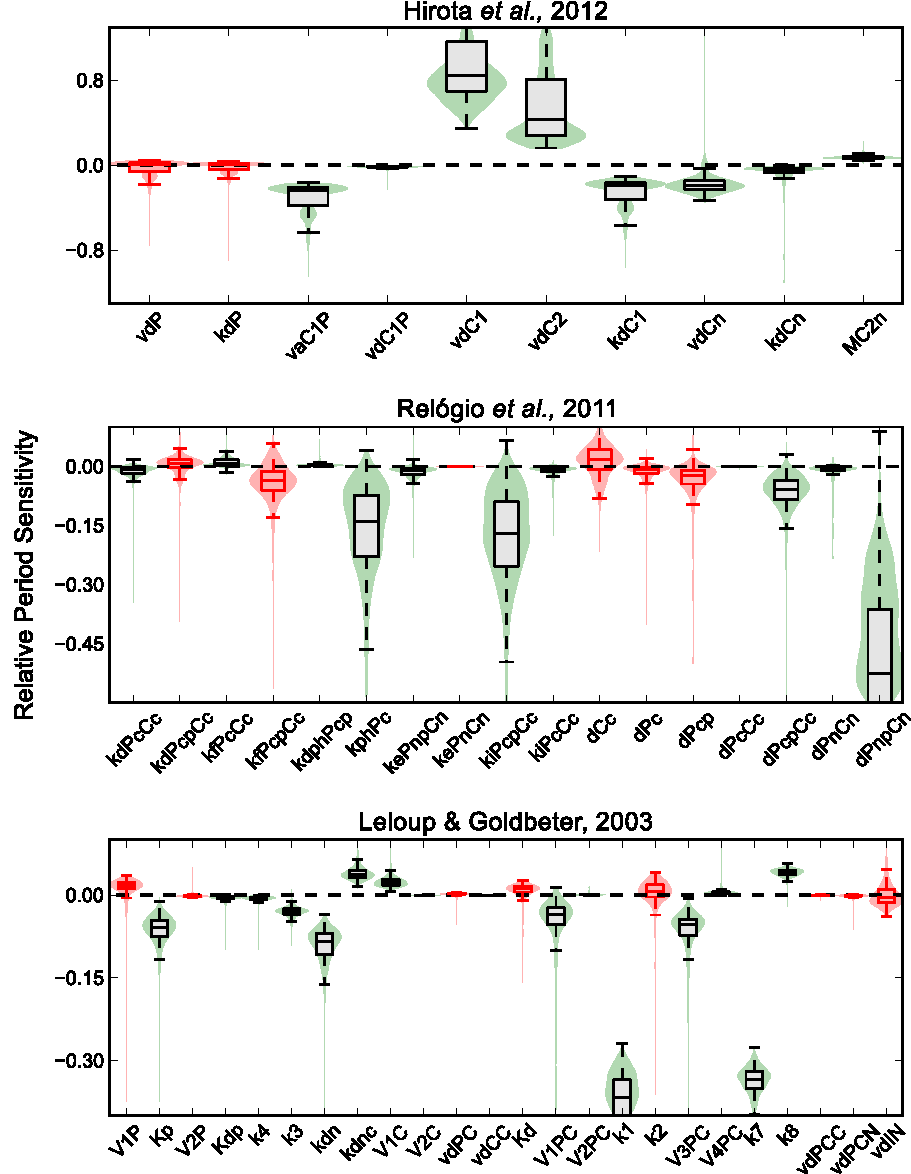
\includegraphics[height=0.7\textheight]{chap4/figures/figS2.pdf}
  \titlecaption{Bootstrap confidence intervals in relative period sensitivities}{Violin plots for distributions in relative period sensitivities for parameters associated with PER and CRY proteins. Whiskers extend to the most extreme data point within 1.5$x$ the inner quartile range.  Distributions in which the 5\textsuperscript{th} and 95\textsuperscript{th} percentile lie on opposite sides of the $x$-axis are colored red and deemed non-identifiable.}
  \label{fig:4.s2}
\end{figure}

\begin{figure}[p]
  \centering
  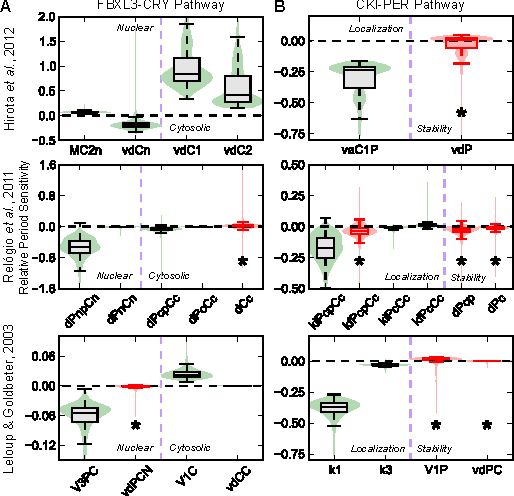
\includegraphics[height=0.6\textheight]{chap4/figures/fig3.pdf}
  \titlecaption{Bootstrap predictions of circadian actions of FBXL3-CRY and CKI-PER pathways}{Violin plots of the relative period sensitivity of parameters associated with potential mechanisms for FBXL3-CRY (A) and CKI-PER (B) activity. A negative or positive period sensitivity indicate that the period of oscillation will increase or decrease when that rate is inhibited, respectively. Distributions that are not different than 0 with 95\% confidence are colored red.  Descriptions of the parameters shown are listed in tables \ref{tab:4.1}-\ref{tab:4.2}.}
  \label{fig:4.3}
\end{figure}

\begin{table}[p]
\caption{Descriptions of the model parameters governing FBXL3-CRY}
\label{tab:4.1}
\centering
\begin{tabular}{llp{10cm}}\toprule
Model              & Parameter & Description \\\midrule
\cite{Hirota2012}  & MC2n      & CRY2 nuclear multiplicative degradation coefficient \\
                   & vdCn      & CRY1/2 nuclear degradation rate \\
                   & vdC1      & CRY1 cytoplasmic degradation rate \\
                   & vdC2      & CRY2 cytoplasmic degradation rate \\\midrule
\cite{Relogio2011} & dPnpCn    & Phosphorylated PER-CRY complex nuclear degradation rate \\
                   & dPnCn     & PER-CRY complex nuclear degradation rate \\
                   & dPcpCc    & Phosphorylated PER-CRY complex cytoplasmic degradation rate \\
                   & dPcCc     & PER-CRY complex cytoplasmic degradation rate \\
                   & dCc       & CRY cytoplasmic degradation rate \\\midrule
\cite{Leloup2003}  & V3PC      & PER-CRY complex nuclear phosphorylation rate \\
                   & vdPCN     & Phosphorylated PER-CRY complex nuclear degradation rate \\
                   & V1C       & CRY cytoplasmic degradation rate \\
                   & vdCC      & Phosphorylated CRY cytoplasmic degradation rate \\\bottomrule
\end{tabular}
\end{table}

\begin{table}[p]
\caption{Descriptions of the model parameters governing CKI-PER}
\label{tab:4.2}
\centering
\begin{tabular}{llp{10cm}}\toprule
Model              & Parameter & Description \\\midrule
\cite{Hirota2012}  & vaC1P   & PER-CRY complex nuclear entry rate \\
                   & vdP     & PER cytoplasmic degradation rate \\\midrule
\cite{Relogio2011} & kiPcpCc & Phosphorylated PER-CRY complex nuclear entry rate \\
                   & kfPcpCc & Phosphorylated PER-CRY complex association rate \\
                   & kiPcCc  & PER-CRY complex nuclear entry rate \\
                   & kfPcCc  & PER-CRY complex association rate \\
                   & dPcp    & Phosphorylated PER cytoplasmic degradation rate \\
                   & dPc     & PER cytoplasmic degradation rate \\\midrule
\cite{Leloup2003}  & k1      & PER-CRY complex nuclear entry rate \\
                   & k3      & PER-CRY complex association rate \\
                   & V1P     & PER cytoplasmic phosphorylation rate \\
                   & vdPC    & Phosphorylated PER cytoplasmic degradation rate \\\bottomrule
\end{tabular}
\end{table}

We next describe parameters potentially associated with CKI-dependent regulation of PER localization and stability. 
Since PER is rate-limiting in the formation of the PER-CRY complex \cite{Lee2001}, rates associated with complex formation or nuclear import were included in this analysis. 
Conversely, we did not include degradation rates of PER-CRY nuclear repressive complex, since CRY alone is considered the main repressor. 
While it was hypothesized in models where PER acts as a direct repressor that the regulation of PER stability would play the dominant role determining the period \cite{Gallego2006, Vanselow2006}, our new assumptions revealed that parameters governing PER degradation showed only non-identifiable responses. 
 However, inhibition of rates associated with the nuclear entry of the PER-CRY complex showed strong period lengthening effects. 
These results indicate that under our current understanding of clock kinetics, the regulation of nuclear import likely plays the prominent role in CKI-dependent period regulation.

\subsection{Independent mechanisms of PER and CRY regulation}
Using \fref{mod:hirota} and the perturbations identified in \fref{fig:4.3}, we first confirmed that inhibition of nuclear CRY degradation (vdCn) and PER-CRY nuclear import (vaC1P) reproduced the experimental period and amplitude effects of the small molecules KL001 and longdaysin, respectively (\fref{fig:44a}, compare with \fref{fig:4-1b}). 

\begin{figure}[h]
  \centering
  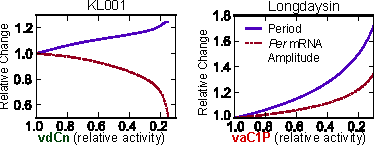
\includegraphics[width=0.7\textwidth]{chap4/figures/fig4a.pdf}
  \titlecaption{Predictions of KL001 and longdaysin results}{{\it In silico} reproductions of the circadian reporter experiments in \fref{fig:4-1b}, using the predictions identified in \fref{fig:4.3}.}
  \label{fig:44a}
\end{figure}

Comparison of the oscillatory profiles of {\it Per} mRNA and nuclear CRY protein (\fref{fig:44b}) revealed that inhibition of FBXL3-dependent CRY degradation caused lingering nuclear CRY to not be completely purged each cycle. 
 This excess repressor during the accumulating phase of {\it Per} and {\it Cry} transcripts resulted in lower E box amplitudes, providing a likely explanation for the effect of KL001.

\begin{figure}[h]
  \centering
  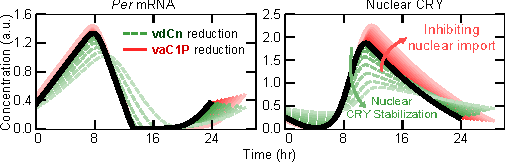
\includegraphics[width=0.85\textwidth]{chap4/figures/fig4b.pdf}
  \titlecaption{Comparison of the effects of KL001 and longdaysin}{Parameter changes were normalized such that the period change was equal for each pair of perturbations (vdCn: 100\% $\to$ 23\%, vaC1P: 100\% $\to$ 51\%).}
  \label{fig:44b}
\end{figure}

In contrast, stabilization of cytoplasmic PER (lowering vdP) resulted in reduced transcriptional amplitude with minimal period effect (\fref{fig:4S3}), consistent with experimental findings from the knockdown of $\beta$-TrCP, an F box protein responsible for PER degradation \cite{Ohsaki2008}. 
However, other experimental results have shown that down-regulation of $\beta$-TrCP leads to longer periods \cite{Reischl2007}, suggesting that further modeling and experimental inquiry is needed on the role of $\beta$-TrCP in clock regulation. 
This period lengthening might be explained through $\beta$-TrCP-mediated stabilization of nuclear PER-CRY or by using alternative kinetic assumptions for the rate of PER-CRY binding. 

\begin{figure}[h]
  \centering
  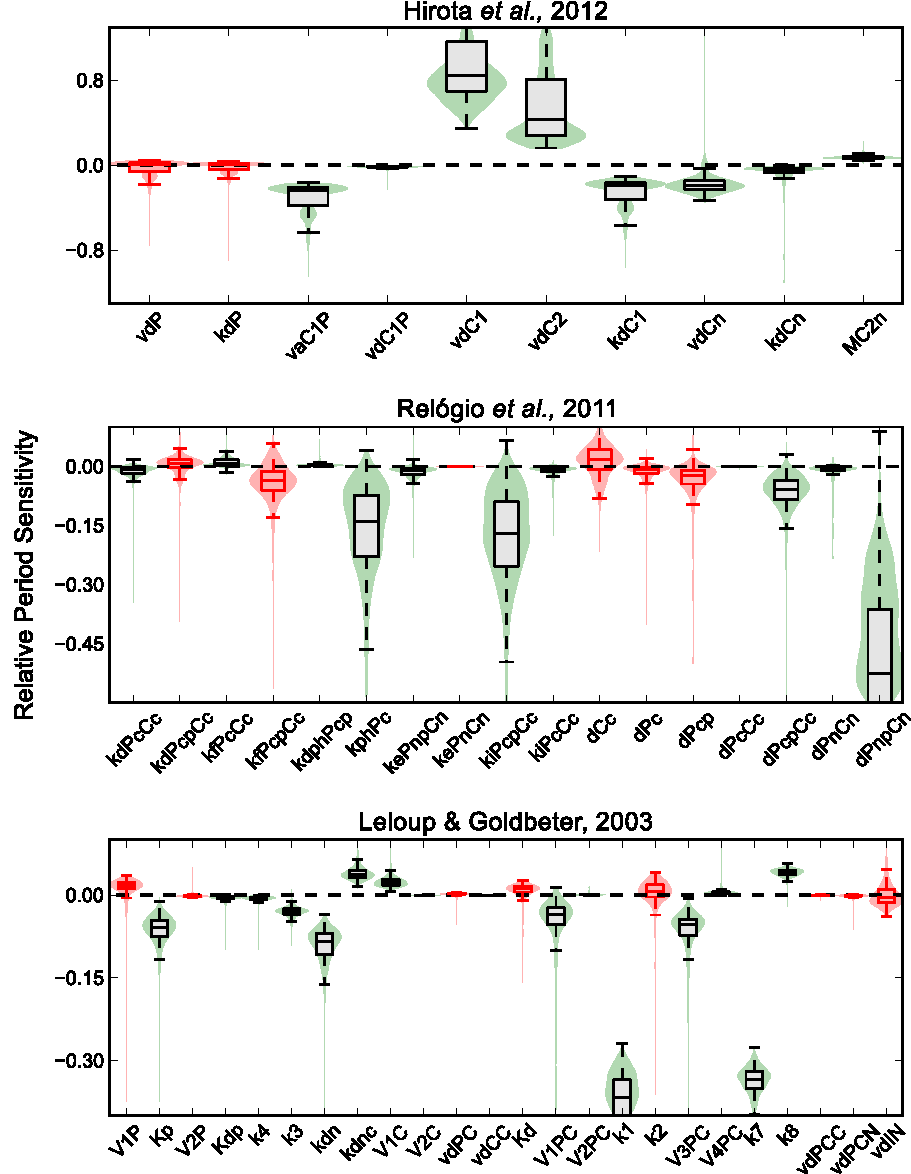
\includegraphics[width=0.6\textwidth]{chap4/figures/figS3.pdf}
  \titlecaption{Effect of cytoplasmic PER stabilization on period and E box transcription amplitude}{Relative period and peak-to-trough amplitude change in {\itshape Per} mRNA resulting from a reduction in the vdP parameter in the model from Hirota {\itshape et al.}, 2012.}
  \label{fig:4S3}
\end{figure}


\subsubsection{CKI likely regulates nuclear entry rather than PER stability}
We further compared the effect of inhibiting PER degradation with inhibiting nuclear import on the oscillatory profile of key clock proteins (\fref{fig:44c}) to identify mechanistic differences between the two potential effects of CKI inhibition. 
Both perturbations increased cytoplasmic PER, suggesting the two mechanisms are difficult to distinguish experimentally. 
Direct stabilization of PER in the cytoplasm (lowering vdP) lead to two simultaneous trends which shift the period in opposite directions: it shortened the time delay between transcription and inactivation by accelerating the accumulation of cytoplasmic PER and nuclear PER-CRY; and lengthened the repressive phase by increasing the total amount of PER-CRY which enters the nucleus. 
These perturbations sped and slowed the clock, respectively, and resulted in little period change. 
In contrast, inhibiting PER-CRY nuclear entry (lowering vaC1P) caused additional free protein to build in the cytoplasm, delaying nuclear accumulation and ultimately increasing the total amount of nuclear PER-CRY. 
Since both of these trends work to increase period length, inhibiting PER-CRY nuclear entry resulted in significantly longer cycles. 
Additionally, the longer cytoplasmic time delay resulted in increased transcription, yielding slightly higher amplitudes (\fref{fig:44b}) that closely match the experimental results of the small molecule longdaysin.

\begin{figure}[h]
  \centering
  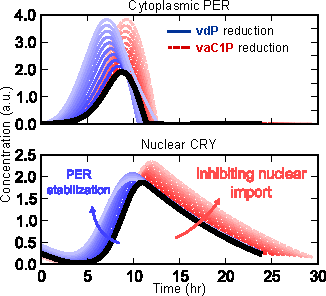
\includegraphics[width=0.6\textwidth]{chap4/figures/fig4c.pdf}
  \titlecaption{Comparison of two candidate mechanisms for CKI inhibition}{Effects of increasing PER stabilization and nuclear import inhibition  on the time profiles of cytoplasmic PER (top) and nuclear CRY (bottom). Parameter values were selected such that the amplitudes of cytoplasmic PER are equal at each level. Lighter colors indicate stronger perturbations (vdP: 100\% $\to$ 22\%, vaC1P: 100\% $\to$ 45\%), $t=0$ is set to the onset of PER accumulation.}
  \label{fig:44c}
\end{figure}


Since CKI likely regulates both stability and subcellular localization of PER {\it in vivo}, we considered the effects of simultaneously lowering both PER cytoplasmic degradation and nuclear entry rates, as shown in \fref{fig:45}.
The loss of oscillations under extreme reduction of both parameters highlights an interesting role of CKI in conferring robustness to the circadian clock: since oscillations are lost when import of the PER-CRY complex to the nucleus ceases to be rhythmic, CKI ensures lingering PER is purged from the cytoplasm by one pathway or another before E box transcription resumes. 
This importance has been proven experimentally, as disruption of CKI-mediated regulation leads to compromised circadian oscillations \cite{Lee2009a}.


\begin{figure}[h]
  \centering
  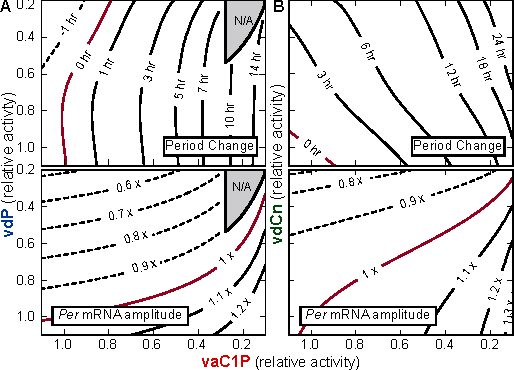
\includegraphics[width=0.9\textwidth]{chap4/figures/fig5.pdf}
  \titlecaption{Independence of CKI-PER and FBXL3-CRY pathways}{({\bfseries A}) Contour plots of period change (top) and {\bfseries Per} mRNA amplitude (bottom) for simultaneous inhibition of both PER degradation (vdP) and nuclear import (vaC1P). The gray shaded region indicates loss of oscillations. ({\bfseries B}) Period and amplitude change contour plots for varying both vdCn (CRY nuclear degradation rate) and vaC1P (PER-CRY nuclear import). The consistently straight lines indicate the independence of CKI-PER and FBXL3-CRY mechanisms.}
  \label{fig:45}
\end{figure}

Together, inhibition of CKI by longdaysin may increase the time required before PER-CRY can enter the nucleus to repress transcription, leading to a higher amplitude and longer period. 
In contrast, KL001 lengthens the period by stabilizing nuclear CRY, resulting in a longer time delay before transcription resumes and lower amplitude from increased E box repression. 
PER regulation through CKI is therefore partitioned to the accumulating phase, controlling the speed and amount of PER-CRY complex that enters the nucleus. 
CRY regulation through FBXL3 is partitioned independently to the repressive phase, controlling the length of time until CLOCK-BMAL1-dependent transcription resumes (\fref{fig:46}). 
This independence was reproduced {\it in silico} by the simultaneous reduction of nuclear CRY degradation and PER-CRY nuclear import (\fref{fig:45}), where nonlinear interactions in amplitude and period between the two perturbations are all but absent.

\begin{figure}[h]
  \centering
  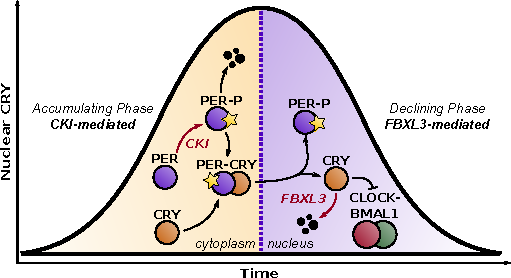
\includegraphics[width=0.8\textwidth]{chap4/figures/fig6.pdf}
  \titlecaption{Spatiotemporal separation underlies independence of CKI-PER and FBXL3-CRY pathways}{Longdaysin, acting through CKI, lengthens the accumulating phase of the circadian cycle, while KL001, acting through FBXL3, lengthens the declining phase.}
  \label{fig:46}
\end{figure}

\section{Discussion}
An understanding of the interactions between posttranslational regulators is crucial for the further development of circadian pharmacological reagents, as efficient modulation of clock function will assuredly come from simultaneous perturbations to many connected species. 
In this study, we used circadian reporter cells together with mathematical modeling to provide mechanistic insight into the differences of CKI- and FBXL3- mediated posttranslational regulation of PER and CRY. 
As a result, we clarified a process by which CKI exerts control over the circadian period, demonstrated through both the hyperphosphorylating CKI$\epsilon^\mathrm{tau}$ mutant and small molecule CKI inhibitors, such as longdaysin. 
In developing our predictions, we have used multiple models and parameterizations to ensure our mechanisms are consistent across many {\it in silico} realizations. 
These results reinforce the notion that computational modeling is essential in interpreting results in systems with complicated oscillatory feedback. 
Additionally, {\it in silico} analyses reveal hidden design principles of biological networks, as this work highlights the importance of the CKI family of kinases in conferring robustness to the circadian cycle. 
 
\subsection{Phase-dependent activity of small molecule modulators}
In this chapter, it was shown that the posttranslational CKI and FBXL3 control separate time regimes of the core clock oscillation. 
While in the cultured cell experiments the small molecule modulators were continuously present, in pharmacological applications there would likely be dosed at specific times of day. 
Since their targets play key roles during specific circadian phases, it is likely that there would be a significant difference in small molecule effect depending on the time at which they are given. 
In the next chapter, I systematically analyze the dynamic consequences associated with {\itshape transient} applications of small molecule agonises, rather than dose-dependent continuous applications, as the former will likely have more significant clinical relevance. 

\chapter[Amplitude metrics for cellular bioluminescence reporters]{Amplitude metrics for cellular bioluminescence reporters\footnote{Portions of this chapter are published in P. C. St. John, S. R. Taylor, J. H. Abel, and F. J. Doyle, ``Amplitude Metrics for Cellular Circadian Bioluminescence Reporters,'' {\itshape Biophys. J.}, vol. 107, pp. 2712– 2722, Dec. 2014.}}
% \section{Motivation, link to previous chapter}\blindtext
% \subsection{Different enzymes control circadian rhythms at different phases}\blindtext
% \subsection{Perturbations likely have a time-dependent effect on amplitude}\blindtext
% \subsection{Comparison of Ukai vs Pulivarthy 2007}\blindtext
% \section{Single cell amplitude metrics}\blindtext
% \subsection{Definition of amplitude metric}\blindtext
% \subsection{Finite difference ARC}\blindtext
% \subsection{Derivation of sensitivity-based method}\blindtext
% \section{Population-level models}\blindtext
% \subsection{Definitions and diffusion-convection equation}\blindtext
% \subsection{Circular statistics}\blindtext
% \subsection{Inverting $p(\theta, \hat{t})$}\blindtext
% \subsection{Calculating $\bar{x}(\hat{t})$ and $\hat{x}(\hat{t})$}\blindtext

\section{Background}

In the previous chapter, I described used mathematical modeling to explain the systems-level effects of two pharmacological agents. 
In doing so, it was shown that each compound controlled reactions which primarily occur during specific times of day. 
Since clinical applications of circadian therapies will likely have a time at which they are administered, it is important to understand the effects of temporary perturbations on circadian amplitude. 
The effects of temporary perturbations are more complicated, however, since they may effect both the single-cell oscillator as well as the synchrony of cell populations as a whole.
In this chapter, I develop the mathematical background required to understand and efficiently predict the response of a population of oscillators to a temporary change.

\subsection{Importance of circadian amplitude}
% In mammals, circadian rhythms are endogenous oscillations in gene transcription responsible for coordinating daily changes in physiology.
While the suprachiasmatic nucleus (SCN) in the brain serves as the body's master pacemaker, cells found in peripheral tissues also oscillate in a circadian manner \cite{Lamia2008}.
These peripheral clocks process systemic and SCN-mediated entraining cues, buffering against rhythmic changes in energy availability to maintain metabolic homeostasis \cite{Kornmann2007}.
The amplitude of circadian transcription is a relevant factor, and has been shown to play a critical role in phase resetting and entrainment \cite{Pittendrigh1991, Abraham2010}.
Recent studies have further highlighted the importance of high peripheral clock amplitudes in maintaining metabolic health.
Mice lacking an intact clock have been shown to develop metabolic disease \cite{Marcheva2010}, while low amplitude clock oscillations, whether caused by diet \cite{Hatori2012} or age \cite{Chang2013} have also been tied to metabolic disorders.
An understanding of how clock amplitudes are regulated is therefore a topic of ongoing research with potential therapeutic applications \cite{St.John2014}.
Unlike the network of oscillators in the SCN, in which intercellular coupling maintains robust amplitudes even in the absence of external cues, peripheral oscillators are thought to lack a direct mechanism to spontaneously synchronize \cite{Welsh2004}.
As a result, populations of peripheral clocks are likely synchronized by common external cues, with stochastic effects and cell heterogeneity driving entrained populations gradually toward desynchrony.

\subsection{Amplitude at the single-cell and population level}
The development of immortalized peripheral oscillator cell lines with bioluminescent reporters has allowed high-throughput analysis of the responses of circadian rhythms to genetic and pharmacological manipulation \cite{Hirota2010, Ramanathan2014}.
In addition to providing experimental tractability, these systems provide detailed information on the amplitude of oscillations in gene transcription, a measure often lacking from earlier experiments using wheel-running activity.
 As a result, these cell lines have proven useful in studying core clock connectivity and stoichiometry \cite{Baggs2009}.
However, since {\itshape in vitro} experiments typically measure entire cultures of cells, data collected at the population-level can obscure the response of the clock at the scale of the gene-regulatory network.
Even when individual cells can be recorded, stochastic noise hinders accurate amplitude determination.
As a result, two studies using similar perturbations to understand the mechanism of light-induced amplitude reduction reached differing conclusions, in which either single-cell amplitude reduction or population-level desynchrony was identified as the dominant factor \cite{Pulivarthy2007, Ukai2007}.

\subsection{Role of mathematical modeling}
Mathematical models have long been used to understand the results of circadian experiments \cite{Leloup2003, Becker-Weimann2004}, aided by definitions and computational techniques designed to match modeling predictions to experimental data.
One such definition is the response function, a general technique that maps a change in an output variable to a temporary change in parameters \cite{Rand2004}.
For instance, the phase response curve (PRC) has been used to characterize the entrainment behavior of both experimental and mathematical systems \cite{Daan1976, Taylor2008, Pfeuty2011}, and in analyzing the synchrony of populations of oscillators \cite{Kim2014}.
Accurate and efficient numerical routines for finding infinitesimal PRCs have therefore been developed \cite{Kramer1984, Gunawan2006, Taylor2008a}.
In addition to changes in phase, phase-dependent changes in amplitude are an important factor in understanding circadian rhythms.
Amplitude response curves (ARCs) were first used in the clock literature to understand the effects of light pulses on simple phase-amplitude models, and were useful in predicting phase singularity behavior \cite{Jewett1998}.
ARCs have also been used to characterize perturbations to groups of oscillators through desynchrony \cite{Achermann1999, Ukai2007}, at the level of the single oscillator \cite{VanderVeen2012, Castejon2013}, and even in studying the effect of entrainment phase on SCN rhythm amplitude \cite{VanOosterhout2012}.
However, previous definitions of the ARC are inconsistent between studies and do not simultaneously consider amplitude effects at the single-cell and population level.

The choice of modeling framework dictates the type of amplitude response which can be predicted.
Ordinary differential equation (ODE) models of gene regulation are capable of describing the amplitude and phase-resetting behavior of single cells, but fail to capture the collective dynamics of a population of oscillators.
Likewise, phase-only models correctly capture the change in synchrony of a population, but do not capture fluctuations in amplitude of individual oscillators.
Explicit stochastic simulations of populations of cells are capable of realistically capturing both single-cell and population-level effects, and have been successfully used to understand the response of coupled oscillators to external VIP perturbation \cite{An2013}.
However, these methods are computationally expensive, and cannot be used for an analytical understanding of amplitude response.

In this chapter, I describe approaches to quantify amplitude change in a population of non-interacting oscillators.
By exploiting the independence of each oscillator, we derive computationally efficient methods to approximate the mean dynamics of full stochastic simulations.
Additionally, our method allows the calculation of ARCs at both the single-cell and population level, allowing the behavior of the system to be quickly profiled.
Specifically, we use ODE models to describe the transient amplitude response at the single-cell level, coupled with a phase probability density function to describe population-level dynamics.
Following a perturbation with a finite duration, a limit cycle oscillator undergoes a transient change in amplitude.
When the mean expression level of a population of oscillators is also considered, an additional change in amplitude is incurred due to the change in synchrony of the population, which persists until synchrony is changed by subsequent perturbations.
We therefore observe a separation in timescales between the effects on clock output mediated at the single-cell level and those mediated by population synchrony, allowing the source of an amplitude change to be qualitatively inferred by inspection of bioluminescence data.
Characterizing the mechanisms and consequences of both types of amplitude regulation will be important in understanding how peripheral amplitudes are maintained, and may lead to the design of pharmacological or behavioral strategies to boost circadian amplitudes.


\section{Methods}

\subsection{Perturbations to limit cycle systems}

In this chapter we restrict our analysis to temporary perturbations capable of entraining an oscillatory system, excluding permanent parameter changes arising, for instance, from genetic knockout experiments.
The most simple entraining perturbation involves adding or removing components to a limit cycle system, resulting in a perturbed trajectory $x(t)$.
Here the initial conditions are determined by the strength of the perturbation and the phase at which it is applied:
\begin{equation}
  x(0) \coloneqq x^\gamma(\theta_0) + \Delta x(0).
  \label{eq:stateperturbation}
\end{equation}
This trajectory evolves according to \fref{eq:odefn}, eventually returning to $x^\gamma$.
It is useful to express this trajectory by the deviation from the limit cycle:
\begin{equation}
  \Delta x(\tilde{t}) = x(\tilde{t}) - x^\gamma(\tilde{t} + \theta_0).
  \label{eq:delxt}
\end{equation}

In addition to perturbations directly to the state of the system, oscillators can also be perturbed by temporary changes to the parameters.
For a parameter pulse $\Delta p$ of duration $\tilde{d}$ (in radians) that ends at $\theta_0$, the oscillator deviates from the limit cycle trajectory according to:
\begin{align}
  x_{\tilde{d}}(-\tilde{d}) &= x^\gamma(\theta_0 - \tilde{d}) \\
  \frac{dx_{\tilde{d}}}{d\tilde{t}} &= \tilde{f}(x_{\tilde{d}}(\tilde{t}), p + \Delta p) \label{eq:ode_pert}.
\end{align}
The pulse trajectory $x_{\tilde{d}}(\tilde{t})$ is then integrated from $\tilde{t} = -\tilde{d} \to 0$, at which point the pulse is removed.
A temporary parameter pulse is therefore equivalent to a state perturbation, but with the perturbation at $t = 0$ defined by:
\begin{equation}
  \Delta x(0) = x_{\tilde{d}}(0) - x^\gamma(\theta_0).
\end{equation}
A schematic depicting an example perturbed and reference trajectory is shown in \fref{fig:51schem}.

\begin{figure}[tbp]
  \begin{center}
    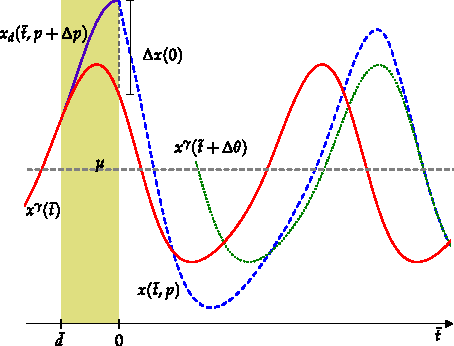
\includegraphics[width=.75\textwidth]{chap5/figures/figure_1_schem.pdf}
  \end{center}
  \titlecaption{Schematic showing trajectories used in the calculation of single-cell phase and amplitude change}{A perturbation $x(\tilde{t},p)$, blue, from the limit cycle solution $x^\gamma(\tilde{t},p)$, red, ultimately returns to the limit cycle with a phase shift $x^\gamma(\tilde{t} + \Delta\theta,p)$, green.}
  \label{fig:51schem}
\end{figure}

\subsection{Phase response curves}
Quantifying phase changes following a perturbation has been well studied and is particularly relevant for models of circadian rhythms \cite{Kramer1984, Taylor2008a}.
A phase response curve (PRC) maps the change in phase resulting from the same perturbation applied at each initial phase.
Infinitesimal PRCs, the derivative of the phase change with respect to the perturbation, can be defined for state and parameter-impulse perturbations \cite{Taylor2008a}.
Methods for efficiently calculating these quantities using ODE sensitivity analysis have been developed \cite{Taylor2008a}, with the important result that the parameter- and state-impulse PRCs can be related by the Jacobian matrix:
\begin{equation}
  \frac{d}{d\tilde{t}}\frac{d\theta}{dp} = \frac{d\theta}{dx}\frac{d\tilde{f}}{dp}.
  \label{eq:pPRCequiv}
\end{equation}
This result follows from the fact that in the limit of an infinitely short and small parameter pulse, $\Delta x(0) \to \nicefrac{d\tilde{f}}{dp}\,\tilde{d}\, \Delta p$.

\subsection{Phase-diffusion model}
Large populations of oscillators are typically described using phase-only models \cite{Rougemont2006}, in which the state of each oscillator is represented only by its phase, $\theta$.
The synchrony of the population can be modeled using a probability density function $p(\theta, \tilde{t})$ that describes the probability of finding an oscillator at each phase \cite{Kuramoto1984}.
The usefulness of probability density functions in describing the phase and amplitude responses of populations of circadian cells has been previously shown \cite{Ukai2007}.
As with all probability density functions,
\begin{equation}
  \int_0^{2\pi} p(\theta, \tilde{t}) \; d\theta = 1.
\end{equation}
The shape of $p(\theta, \tilde{t})$ changes as the cells advance in time.
Stochastic effects cause the population to gradually desynchronize as slight cycle-to-cycle deviations are propagated throughout the population \cite{Teramae2004}.
For a infinite population of oscillators, these effects are well-described by a Fokker-Plank equation \cite{Stein1965}:
\begin{equation}
  \frac{\partial p}{\partial \tilde{t}} = \frac{\partial p}{\partial \theta} + d\frac{\partial^2 p}{\partial \theta^2}.
  \label{eq:pde}
\end{equation}
Due to the rescaling of $t$, the mean period of the population is $2\pi$.
Here, the $\nicefrac{\partial p}{\partial \theta}$ term, analogous to convection, describes the mean oscillatory period, while the $\nicefrac{\partial^2 p}{\partial \theta^2}$ term describes the diffusion of phases across $[0, 2\pi)$.
The phase diffusivity parameter $d$ (in units of inverse radians) describes the speed with which the population desynchronizes and can be fit to experimental data \cite{Rougemont2007}.
\fref{eq:pde} has periodic boundary conditions, with initial condition $\phi(\theta)$ as the phase population at $t=0$:
\begin{align}
  \text{BCs:}\quad p(0, \tilde{t}) &= p(2\pi, \tilde{t}) \\
  \frac{\partial p}{\partial \theta}(0, \tilde{t}) &= \frac{\partial p}{\partial \theta}(2\pi, \tilde{t}) \\
  \text{IC:}\quad p(\theta, 0) &= \phi(\theta).
  \label{eq:pde_ic}
\end{align}
The solution of equations~(\ref{eq:pde}-\ref{eq:pde_ic}) is well-characterized, with $p(\theta, \tilde{t})$ evolving in time as the convolution of the initial conditions with a wrapped normal distribution with mean $\tilde{t}$ and standard deviation $\sqrt{2d\tilde{t}}$ \cite{Chirikjian2009}:
\begin{equation}
  p(\theta, \tilde{t}) = \phi(\theta) * \mathcal{WN}(\theta; \tilde{t},
  \sqrt{2\, d\, \tilde{t}}),
\end{equation}
in which the wrapped normal distribution \cite{Mardia2009} is defined as
\begin{equation}
  {\cal WN}(\theta; \mu, \sigma) =
  \frac{1}{\sigma\sqrt{2\pi}}\sum_{k=-\infty}^\infty \exp\left[\frac{-(\theta
  - \mu + 2\pi k)^2}{2\sigma^2}\right].
  \label{eq:wrapped_normal}
\end{equation}
Since the convolution of two normal distributions is also a normal distribution, it is efficient when possible to describe $\phi(\theta)$ as a normal distribution with mean $\mu_0$ and standard deviation $\sigma_0$, such that $p(\theta, \tilde{t})$ can be found analytically through
\begin{equation}
  p(\theta, \tilde{t}) = \mathcal{WN}(\theta; \mu_0 + \tilde{t},
  \sqrt{\sigma_0^2 + 2d^2\tilde{t}^2}).
\end{equation}

\subsection{Numerical simulations}

ODE models were simulated in Python, using the computer algebra package CasADi \cite{Andersson2013b}.
Stochastic simulations were performed using the StochKit2 package \cite{Sanft2011a}.
The codes used to generate the figures are included as a supplemental file.

\section{Results}

A signal to a population of limit cycle oscillators can affect amplitude in two ways.
First, individual cells are perturbed from their limit cycles, and exhibit transient dynamics before settling back to steady state amplitudes.
Secondly, the phases of the population are changed, resulting in a permanent change in population synchrony.
Differences between these two types of amplitude change are summarized in \fref{fig:arcdiff}.
Therefore, in order to derive continuous approximations to the dynamics of a large population of non-interacting oscillators, we first demonstrate how ARCs can be found at both the single-cell and population level.

\begin{figure}[tbp]
  \centering
  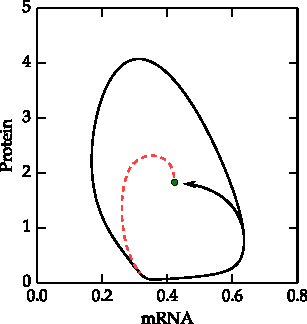
\includegraphics[width=0.45\textwidth]{chap5/figures/arc_singlecell.pdf}
  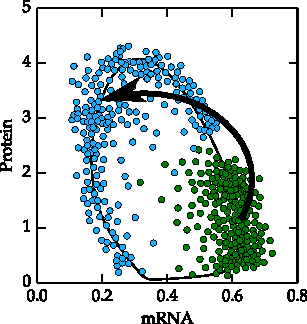
\includegraphics[width=0.45\textwidth]{chap5/figures/arc_population.pdf}
  \titlecaption{Differences between population and single-cell mediated amplitude change}{Amplitude change at the single-cell level (left) is temporary, mediated by the dynamics of the limit cycle system. At the population-level (right), many limit cycle oscillators are averaged together to find the total expression level. The amplitude is therefore changed by the degree of synchrony of the population, which is often changed by perturbations.}
  \label{fig:arcdiff}
\end{figure}

\subsection{Definition of an amplitude metric at the single-cell level}

Following a perturbation to a single cell, the path that the perturbed trajectory $x(t)$ takes in returning to the limit cycle will have a different amplitude than the unperturbed trajectory.
While such an amplitude change will only have a finite duration, it plays an important role when perturbations are repeatedly received by the clock, such as a peripheral oscillator entrained to daily metabolic stimuli.
To define an amplitude change metric for such a case, we compare a perturbed trajectory $x(t)$ to a phase-shifted limit cycle reference $y(t)$, for which $x(t) \to y(t)$ for sufficiently long times.
Since $x(t)$ approaches the reference as $t \to \infty$, the means of both trajectories are equal and can be calculated by
\begin{equation}
  \mu \coloneqq \int_0^{2\pi} \frac{x^\gamma(\theta)}{2\pi} \; d\theta.
  \label{eq:mu}
\end{equation}
The amplitude change metric is defined as
\begin{equation}
  \begin{aligned}
    \Delta A (x(t), y(t)) &\coloneqq \int_0^\infty (x(t) - \mu)^2 - (y(t) - \mu)^2 \; dt\\
    &= \int_0^\infty h(t) \; dt.
  \end{aligned}
  \label{eq:ampchangedefinition}
\end{equation}
This amplitude metric was chosen over alternatives, such as peak-trough distance, for its analytical tractability.
The integrand in \fref{eq:ampchangedefinition}, abbreviated by $h(t)$, compares the variances of the reference and perturbed trajectories.
When $h(t) > 0$, the trajectory is further from the mean than the reference, and similarly when $h(t) < 0$ the trajectory is closer to the mean than the reference.
Thus the overall amplitude change can be calculated by integrating $h(t)$ until the two trajectories converge, returning an amplitude value for each state variable.
Amplitude change for a two-dimensional oscillator is easy to visualize graphically.
In \fref{fig:51b}, the same state perturbation $\Delta x(0)$ applied at two different phases results in opposite amplitude changes, depending on whether the perturbation shifts the trajectory to the interior of the limit cycle (reduced amplitudes) or to the outside the limit cycle (increased amplitudes).
Trajectories for the second state variable, $Y(\tilde{t})$, and the corresponding integrand for the amplitude change equation, $h(\tilde{t})$, demonstrate how this transient change is quantified.

\begin{figure}[tbp]
  \begin{center}
    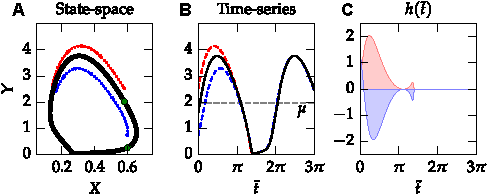
\includegraphics[width=.75\textwidth]{chap5/figures/figure_1_b.pdf}
  \end{center}
  \titlecaption{Amplitude metrics at the single-cell level measure transient deviations from the limit cycle}{The same perturbation applied at two different phases can result in opposite amplitude effects. The state-space representation ({\bfseries B}) reveals the path both perturbations take to return to the limit cycle. The time-series representation ({\bfseries C}) shows how the perturbation in blue results in an amplitude decrease, while the one in red results in an amplitude increase. ({\bfseries D}) This amplitude change is quantified by integrating $h(\tilde{t})$, the difference in variance from each solution to the limit cycle as defined in \fref{eq:ampchangedefinition}, from $t=0 \to \infty$. Here the shaded region indicates the area under the curve, $\Delta A$, for the perturbations shown in red and blue. Model adapted from \cite{Novak2008}.}
  \label{fig:51b}
\end{figure}

\subsection{Single-cell amplitude response curves}
Similar to the PRC, we denote the phase-dependent amplitude change following a perturbation as an amplitude response curve (ARC), using the metric presented in \fref{eq:ampchangedefinition}.
In \fref{fig:52}, we calculate the PRC and ARC for a state perturbation of three different strengths.
The weakest perturbation results in type 1 (weak) resetting, in which the phase response curve is continuous, while the strongest perturbation results in type 0 (strong) resetting, in which the PRC is discontinuous.
This transition occurs once the state perturbation is strong enough to push the trajectory over the unstable fixed point located at the middle of the limit cycle.
For a perturbation of intermediate strength, at a critical phase the trajectory will be pushed close to the fixed point and take a long time to recover the steady state amplitude.
The behavior at this singularity point is indicated by a sharp dip in the ARC for this perturbation strength.

\begin{figure}[tbp]
  \centering
  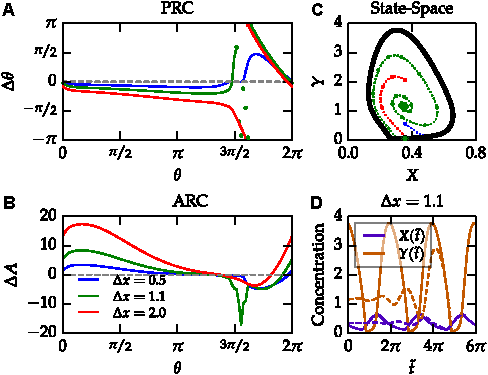
\includegraphics[width=.75\textwidth]{chap5/figures/figure_2.pdf}
  \titlecaption{Phase and amplitude response curves describe how a single oscillator will respond to a perturbation}{({\bfseries A-B}) The phase and amplitude response curves for three perturbations of increasing strengths demonstrate the transition from type 1 phase resetting for a weak stimulus (blue) to type 0 phase resetting from a strong stimulus (red). ({\bfseries C}) The state space representation for the perturbations of varying strengths demonstrate how the trajectories return to the limit cycle. For the particular perturbation shown in green, the trajectory starts very close to the singularity, and therefore takes a long time to recover. ({\bfseries D}) For an oscillator perturbed to the singularity, a strong amplitude reduction ensues. Here, the oscillator with an initial phase $\theta \approx \nicefrac{3\pi}{2}$ is perturbed by $\Delta x = 1.1$ at $\tilde{t} = 0$. Several cycles are required for normal amplitudes to be restored, corresponding to a dip in the ARC (C, green).}
  \label{fig:52}
\end{figure}

Infinitesimal versions of response curves are often more general and easier to compute than those that track a specific perturbation strength \cite{Rand2004}.
We therefore derive an expression for the infinitesimal ARC, defined as
\begin{equation}
  \frac{dA}{dx} \coloneqq \lim_{\Delta x(0) \to 0} \frac{\Delta A\left(x(\tilde{t}),\ x^\gamma(\tilde{t} + \theta_0 + \Delta\theta)\right)}{\Delta x(0)} = \int_0^\infty \lim_{\Delta x(0) \to 0} \frac{h(t)}{\Delta x(0)} \; dt.
  \label{eq:sARC}
\end{equation}
While this quantity could be calculating by using a very small $\Delta x(0)$, it is more accurate and efficient to derive a direct method to calculate \fref{eq:sARC} using the ODE sensitivities defined in \fref{eq:odesens}.
For simplicity, we define $t_\theta = \tilde{t} + \theta_0$, which allows the time variable for the perturbation to vary from $0 \to \infty$ while tracking the appropriate phase on the limit cycle.
Since $\Delta \theta \to 0$ as $\Delta x(0) \to 0$, we Taylor expand the limit cycle trajectory around $t_\theta$:
\begin{align}
  x^\gamma(t_\theta + \Delta\theta) &= x^\gamma(t_\theta) +
  \frac{dx^\gamma(t_\theta)}{d\theta}\Delta\theta + O(\Delta\theta^2)\\
  &= x^\gamma(t_\theta) + \tilde{f}\left(x^\gamma(t_\theta)\right)\Delta\theta +
  O(\Delta\theta^2).
\end{align}
Simplifying the integrand in \fref{eq:sARC},
\begin{align}
  \frac{h(t)}{\Delta x(0)} &= \frac{1}{\Delta x(0)} \left[\left(x^\gamma(t_\theta) + \Delta x(\tilde{t}) - \mu\right)^2 - \left(x^\gamma(t_\theta + \Delta \theta) - \mu\right)^2 \right]\\
  &= \frac{1}{\Delta x(0)} \left[\left(x^\gamma(t_\theta) + \Delta x(\tilde{t}) - \mu\right)^2 - \left(x^\gamma(t_\theta) + \tilde{f}\left(x^\gamma(t_\theta)\right)\Delta\theta - \mu\right)^2 \right]\\
  &= \frac{1}{\Delta x(0)} \left[\left(\Delta x(\tilde{t}) - \tilde{f}\left(x^\gamma(t_\theta)\right)\Delta\theta\right) \left(\Delta x(\tilde{t}) + \tilde{f}\left(x^\gamma(t_\theta)\right)\Delta\theta + 2(x^\gamma(t_\theta) - \mu)\right) \right].
\end{align}
Taking the limit of this integrand as $\Delta x(0) \to 0$ cancels several differential terms, and allows the remainder to be substituted with quantities that can be calculated using ODE sensitivity analysis:
\begin{align}
  \lim_{\Delta x(0) \to 0} \frac{h(t)}{\Delta x(0)} &= 2\left(\lim_{\Delta x(0) \to 0}\frac{\Delta x(\tilde{t})}{\Delta x(0)} - \tilde{f}\left(x^\gamma(t_\theta)\right)\lim_{\Delta x(0) \to 0}\frac{\Delta\theta}{\Delta x(0)}\right) \left(x^\gamma(t_\theta) - \mu\right)\\
  &= 2\left(S(\tilde{t}) - \tilde{f}(x^\gamma(t_\theta))\frac{d\theta}{dx}\right)\left(x^\gamma(t_\theta) - \mu\right).
  \label{eq:sens_sub}
\end{align}
Note that in \fref{eq:sens_sub}, $\nicefrac{d\theta}{dx}$ represents the derivative of $\Delta\theta$ with respect to the perturbation, and is therefore a scalar quantity.
The infinitesimal state-impulse ARC may therefore be calculated directly from the ODE sensitivity matrix and the PRC, allowing the amplitude change for an infinitesimal perturbation to be calculated exactly and efficiently:
\begin{equation}
  \frac{dA}{dx} = \int_0^\infty 2\left(S(\tilde{t}) - \tilde{f}(x^\gamma(t_\theta))\frac{d\theta}{dx}\right)\left(x^\gamma(t_\theta) - \mu\right) \; dt.
  \label{eq:siARC}
\end{equation}
Here, the first term of the integrand $(S - \tilde{f}\dot{\theta})$ tracks the distance from the perturbed trajectory to the limit cycle, which decays to zero as $t \to \infty$.
The second term $(x^\gamma - \mu)$ weights this distance by whether or not the deviation occurs above or below the oscillatory mean, yielding negative amplitude changes when the trajectory is perturbed closer to the mean.
Just as with the parameter-impulse PRC, the infinitesimal parameter-impulse ARC is defined as
\begin{equation}
  \frac{d}{d\tilde{t}}\frac{dA}{dp} \coloneqq \lim_{\tilde{d},\; \Delta p \to 0} \frac{\Delta A}{\tilde{d}\, \Delta p},
\end{equation}
and may be calculated from the state-impulse version with the following relationship:
\begin{equation}
  \frac{d}{d\tilde{t}}\frac{dA}{dp} = \frac{dA}{dx}\frac{d\tilde{f}}{dp}.
    \label{eq:piARC}
\end{equation}
As with \fref{eq:pPRCequiv}, this equivalency reflects the fact that for a pulse of infinitely short duration, a parameter change is equivalent to changing the state of the system along the direction specified by the Jacobian.
Convergence between the methods in equations~(\ref{eq:siARC}-\ref{eq:piARC}) and finite-difference approaches is shown in \fref{fig:5s1}, which demonstrates that the numerically-efficient differential ARCs remain representative even for moderate-strength perturbations.

\begin{figure}[tbp]
  \centering
  \includegraphics[width=.75\textwidth]{chap5/figures/figure_S1.pdf}
  \titlecaption{Convergence of finite-difference and differential methods}{({\bfseries A}) Perturbations of decreasing strength to the state of the oscillator result in phase and amplitude response curves that match the differential limit. ({\bfseries B}) Temporary perturbations of decreasing strength to a kinetic parameter. The duration of each perturbation is fixed to 0.2 radians. Finite difference approximations closely match the differential method, which is offset in phase by 0.1 radians to account for the nonzero pulse duration.}
  \label{fig:5s1}
\end{figure}


\subsection{Population-level response curves}

We next briefly describe how to calculate the PRC and ARC for a phase-density model.
These approaches are commonly used in understanding phase models \cite{Kuramoto1984, Ukai2007}, and are presented here to match previous definitions for single cells. 
A phase transition curve, $g(\theta) = \theta + \Delta\theta$, maps the phase of an oscillator before perturbation to its phase after the perturbation.
We denote the phase probability density function following a perturbation as $\hat{p}(\theta, \tilde{t})$, as shown in \fref{fig:phatdef}.

\begin{figure}[tbp]
  \centering
  \includegraphics[width=.5\textwidth]{chap5/figures/phat.pdf}
  \titlecaption{Perturbations change population-level phase synchrony}{A perturbation giving rise to a phase transition curve $g(\theta)$ results in a changed phase probability density function, denoted as $\hat{p}(\theta, \tilde{t})$}
  \label{fig:phatdef}
\end{figure}

Since individual oscillators are neither created nor destroyed during the perturbation, it is possible - yet numerically difficult - to directly calculate the phase probability distribution following perturbation using the standard change of variables relation:
\begin{equation}
  \hat{p}(\theta, \tilde{t})\; dg(\theta) = p(\theta, \tilde{t})\; d\theta.
  \label{eq:pdfinversion}
\end{equation}
However, it is easier to estimate the mean and standard deviation of the perturbed population $\hat{p}(\theta, \tilde{t})$ using directional statistics \cite{Mardia2009}.
A population defined on the unit circle can be described by a complex variable $z = \rho e^{i\bar{\theta}}$, where $\bar{\theta}$ is the mean phase and $\rho$, the synchronization index, is related to the standard deviation of the population.
For $\rho = 1$, the population is clustered about one mean phase, while for $\rho = 0$ the population is evenly balanced across the unit circle.
Complex variables for the population before and after perturbation can be calculated via
\begin{align}
  z &\coloneqq \int_0^{2\pi} e^{i\theta} p(\theta, \tilde{t}) \; d\theta \label{eq:zbar}\\
  \hat{z} &\coloneqq  \int_0^{2\pi} e^{i\theta} \hat{p}(\theta, \tilde{t}) \; d\theta = \int_0^{2\pi} e^{i g(\theta)} p(\theta, \tilde{t}) \; d\theta.
  \label{eq:zhat}
\end{align}
In \fref{eq:zhat}, we avoid calculating the perturbed population explicitly by instead integrating over the new phases at the prior population density function.
Population-level amplitude and phase responses can therefore be calculated by
\begin{align}
  \Delta \bar{\theta} &= \angle z - \angle \hat{z} \\
  \Delta \rho &= |z| - |\hat{z}|.
  \label{eq:popampchange}
\end{align}
Population-level PRCs and ARCs can be tabulated by solving equations~(\ref{eq:zbar}-\ref{eq:popampchange}) for populations $p(\theta, \tilde{t})$ with different mean phases.
It is important to note that the ARC at the population level strongly depends on the slope of the PRC, as has been shown previously \cite{Ukai2007}.


\subsection{Population-level mean expression profiles}

To efficiently capture the population-level effects of bioluminescence experiments, we couple the detailed single-cell ODE model to a phase-density model.
Previous work has used limit cycle models to estimate population-level parameters, such as desynchronization rate, for phase-only models \cite{Rougemont2007}.
In this chapter, we use an ODE model to calculate the response to a perturbation at each phase, and subsequently take the weighted average of these responses according to the phases of the cells in the population.

Assuming each oscillator in the population follows the dynamics described by $x^\gamma(\theta)$, the unperturbed mean population-level expression, $\bar{x}(\tilde{t})$, can be found by taking the weighted average of the expression level over the current population:
\begin{equation}
  \bar{x}(\tilde{t}) = \int_0^{2\pi} x^\gamma(\theta) p(\theta, \tilde{t}) \; d\theta.
  \label{eq:xbar}
\end{equation}

Phase-diffusion models can explain why the gradual damping from experimental population-level data closely resembles an exponentially damped sinusoid, a result that has been shown experimentally \cite{Welsh2004} and computationally \cite{Rougemont2007}.
Our method similarly demonstrates exponential decay: for the idealized system $x^\gamma(\theta) = \cos(\theta)$ starting from a synchronized state:
\begin{align}
  \bar{x}(\tilde{t}) &= \frac{1}{\sqrt{4\pi d\tilde{t}}}\int_{-\infty}^{\infty} \cos(x) \exp\left(-\frac{(x - \tilde{t})^2}{4d\tilde{t}}\right)\; dx \\
  &= \Re\left[\frac{1}{\sqrt{4\pi d\tilde{t}}}\int_{-\infty}^{\infty} \exp(ix) \exp\left(-\frac{(x - \tilde{t})^2}{4d\tilde{t}}\right)\; dx\right] \\
    &= \Re\left[e^{(i - d)\tilde{t}}\right]\\
    &= e^{-d\tilde{t}} \cos(\tilde{t}).
    \label{eq:expsin}
\end{align}
Due to the smoothing effect of phase diffusion, higher frequency sinusoidal components of the limit cycle are damped faster than lower frequency components, resulting in an exponentially decaying sinusoids even for limit cycles that are not sinusoidal in sufficiently disperse populations.
The analytical result in \fref{eq:expsin} allows us to easily estimate the phase diffusivity parameter in \fref{eq:pde} by simply fitting an exponentially damped sinusoid to detrended bioluminescence data.

Using our continuous approximation to population-level dynamics, we demonstrate an example unperturbed trajectory using a model adapted from \cite{Novak2008}, see \fref{mod:novak}.
In \fref{fig:53}, an initially jagged population density smooths and widens over time as cells desynchronize, similar to the effects of diffusion.
While each cell's expression level follows the limit cycle, the population amplitude gradually damps with time as cells with diverse phases are averaged together.

\begin{model}
  \titlecaption{Model adapted from Nov\'{a}k \& Tyson, 2008 \cite{Novak2008}}{Used for ARC demonstrations in figures \ref{fig:51b}-\ref{fig:53} ($P=4$) and \fref{fig:5s2} ($P=2$). It should be noted that the use of the stochastic simulation algorithm for reactions with non-elementary propensities may inaccurately represent the noise of the full system. In this case, we simply fit the noise characteristics of the approximated model (using the volume parameter) to yield physiologically realistic desynchronization rates. The volume of the stochastic simulations was chosen as $\Omega = 250$.}
  \centering
  \begin{align*}
    \frac{dX}{dt} &= \frac{1}{1 + Y} - X \\
    \frac{dY}{dt} &= k_t \; X - k_d \; Y - \frac{Y}{\alpha_0 + \alpha_1 \; Y +
    \alpha_2 Y^2}
  \end{align*}

  \tablehead{\toprule Parameter & Value\\\midrule}
  \begin{supertabular}{rl}
    $k_t$ & 20 \\
    $k_d$ & 1  \\
    $P$   & 4 (or 2)  \\
    \bottomrule\end{supertabular}\hspace{3ex}
  \begin{supertabular}{rl}
    $\alpha_0$ & 0.005 \\
    $\alpha_1$ & 0.05  \\
    $\alpha_2$ & 0.1   \\
    \bottomrule\end{supertabular}
  \label{mod:novak}
\end{model}

\begin{figure}[tbp]
  \centering
  \includegraphics[width=.75\textwidth]{chap5/figures/figure_3.pdf}
  \titlecaption{Synchrony affects population-level amplitude}{ ({\bfseries A}) Stochastic fluctuations cause a population of cells to gradually desynchronize with time. The phase probability density, $p(\theta, \tilde{t})$, gradually widens as it advances in phase according to the mean period. ({\bfseries B}) The mean amplitude from a population of oscillators is determined by the probability density function $p(\theta, \tilde{t})$ and the oscillator's limit cycle $x^\gamma(\theta)$. As time passes, population-level rhythms resemble an exponentially damped sinusoid.}
  \label{fig:53}
\end{figure}

Next we describe how to calculate population-level mean expression following a perturbation.
The perturbed trajectory $\hat{x}(\tilde{t})$ can be decomposed into contributions from two sources.
First, for long times after the perturbation, each individual oscillator will have returned to the limit cycle $x^\gamma(\theta)$, but with a new population density $\hat{p}(\theta, \tilde{t})$.
This steady-state perturbed trajectory $\hat{x}_{ss}(\tilde{t})$ can be found by
\begin{equation}
  \hat{x}_{ss}(\tilde{t}) = \int_0^{2\pi} x^\gamma(\theta) \hat{p}(\theta, \tilde{t}) \; d\theta.
  \label{eq:xhatss}
\end{equation}
For very long times following perturbation, the new phase probability density could be approximated using the initial mean and standard deviation found through \fref{eq:zhat}, as jagged profiles in the population density will eventually smooth to a normal distribution.
However, for shorter times following perturbation, $\hat{p}(\theta, \tilde{t})$ must be calculated numerically.

The second contribution to the perturbed population trajectory comes from deviations from limit cycle oscillations in each cell.
We calculate the population-level effect of these deviations by averaging over the deviations that occur at each phase.
We define the deviation trajectory $\delta x(\theta, \tilde{t})$ for each phase as the distance between the perturbed trajectory and the phase-adjusted reference:
\begin{align}
  \delta x(\theta_0, \tilde{t}) &\coloneqq x(\tilde{t}) - x^\gamma(\tilde{t} + \theta_0 + \Delta \theta) \\
  \therefore\; \lim_{\tilde{t} \to \infty} \delta x(\theta, \tilde{t}) &= 0.
  \label{eq:deviation}
\end{align}
Since the perturbed trajectory ultimately converges with the phase-adjusted reference, deviations will converge to zero.
Since the phase change, $\Delta\theta$, associated with a perturbation at each phase is likely not known prior to calculating the perturbed trajectory, it is difficult to tabulate deviation trajectories associated with each final phase, $\theta_0 + \Delta\theta$.
It is therefore more straightforward to find the average effect of single-cell perturbations at the population level by weighting the deviations by the phase density function prior to perturbation.
The population-level response to a perturbation, $\hat{x}(\tilde{t})$, is therefore defined as
\begin{equation}
  \hat{x}(\tilde{t}) = \int_0^{2\pi} x^\gamma(\theta)\hat{p}(\theta, \tilde{t}) + \delta x(\theta, \tilde{t})p(\theta, \tilde{t}) \; d\theta.
  \label{eq:xhat}
\end{equation}
Here the first term is equivalent to $\hat{x}_{ss}(\tilde{t})$, the steady-state perturbed trajectory, while the second term decays to zero as individual oscillators return to their steady-state amplitude.
The accuracy of the continuous phase-diffusion model was tested by explicitly simulating a perturbation to a population of 225 uncoupled oscillators using a stochastic simulation algorithm \cite{Gillespie1977, Sanft2011a}.
Good agreement between the stochastic population and continuous approximation was shown in phase shift, single-cell level amplitude change, and alteration of population synchrony (\fref{fig:5s2}).
These results indicate the use of a continuous probability function is justified in the case of cultured cellular reporter systems, which may contain up to $10^5$ individual cells per culture \cite{Welsh2004}.
In addition, the method was verified by similar simulations using the Oregonator \cite{Field1974}, a model containing only mass-action terms, and a detailed mechanistic model of circadian rhythms \cite{Hirota2012} at a variety of phase timings (\fref{fig:5s3a} and \fref{fig:5s3b}).
Good agreement is seen between the continuous and stochastic simulations, indicating the proposed method is suitable for predicting the population-level responses for a variety of model types. 
The slightly reduced accuracy seen in the larger \fref{mod:hirota} demonstrates a limitation of the method, which should be considered before applying the method to extreme cases. 
As \fref{eq:deviation} tabulates the response of the system from the limit cycle, systems which are perturbed from states far from the deterministic limit cycle will not be captured appropriately. 
Therefore, the difference in accuracy between \fref{mod:hirota} and \fref{mod:oregon} likely comes from increased deviation about the deterministic limit cycle in a greater number of spatial dimensions. 
The continuous approximation is therefore able to capture the population-level dynamics of a wide variety of limit cycle models and perturbations.

\begin{figure}[tbp]
  \centering
  \includegraphics[width=.75\textwidth]{chap5/figures/figure_S2.pdf}
  \titlecaption{Approximation of an explicit stochastic population by continuous methods}{({\bfseries A}) A population of 225 stochastic oscillators was simulated using the Gillespie stochastic simulation algorithm (SSA). The mean protein expression, $Y$, is plotted as a function of time. A $50\%$ reduction in the protein translation rate to each of the oscillators is applied from $\hat{t} = -\nicefrac{\pi}{4} \to 0$, resulting in both single-cell and population-level amplitude change (red solid line). This population is approximated by the continuous methods described in this manuscript, in which the decay parameter $d=0.025$ is estimated to match the stochastic-induced desynchrony of the control population (black solid line). The initial standard deviation $\sigma_0 = 0.48$ is similarly matched to the stochastic population. The resulting predicted unperturbed and perturbed trajectories, $\bar{x}(\hat{t})$ and $\hat{x}(\hat{t})$ respectively, closely match the stochastically modeled values.  ({\bfseries B}) Phase histograms for the stochastic population are shown at several phases, both before and after the desynchronizing perturbation.  Phase probability-density functions for the continuous approximation are also shown, with close agreement between stochastic and continuous simulations. This close approximation validates the use of ODE models and phase-diffusion populations in deriving amplitude and phase-response behavior for networks of uncoupled cells.}
  \label{fig:5s2}
\end{figure}

\begin{figure}[tbp]
  \centering
  \includegraphics[width=0.75\textwidth]{chap5/figures/figure_S3a.pdf}
  \titlecaption{Validation of continuous methods with the Oregonator model}{ ({\bfseries A}) The Oregonator model (\fref{mod:oregon}) was tested as an example of a mass-action limit cycle oscillator. A population of 2000 oscillators was perturbed at size different mean phases, $\mu$, by increasing the $\mathit{c2}$ parameter by $50\%$ for $d=\pi$ (highlighted region). Only the average $\mathit{Y2}$ variable is plotted.}
  \label{fig:5s3a}
\end{figure}

\begin{figure}[tbp]
  \centering
  \includegraphics[width=0.75\textwidth]{chap5/figures/figure_S3b.pdf}
  \titlecaption{Validation of continuous methods with the model from Hirota {\itshape et al.,} 2012}{ ({\bfseries A}) ({\bfseries B}) The model described in \cite{Hirota2012} (\fref{mod:hirota}) was similarly tested at a variety of mean phases by reducing the $\mathit{vdp}$ parameter by $28.5\%$ and plotting the resulting $\mathit{c2}$ state variable (as in \fref{fig:55}). Parameters for the continuous approximations were found by estimating the phase, initial standard deviation, period, and phase diffusivity of the control population. }
  \label{fig:5s3b}
\end{figure}


\begin{model}[p]
  \titlecaption{The Oregonator model \cite{Field1974}}{The parameters used are as presented in \cite{Gillespie1977}. Used in \fref{fig:5s3a} as an example of a limit cycle oscillator using only mass-action kinetics.}
  \label{mod:oregon}

  The individual chemical reactions (used for stochastic simulation) are:
\begin{align*}
  X_1 + Y_2 &\xrightarrow{c_1} Y_1\\
  Y_1 + Y_2 &\xrightarrow{c_2} Z_1\\
  X_2 + Y_1 &\xrightarrow{c_3} 2Y_1 + Y_3\\
  2Y_1 &\xrightarrow{c_4} Z_2\\
  X_3 + Y_3 &\xrightarrow{c_5} Y_2
\end{align*}

These reactions can be converted to a standard ODE model, in which only the
intermediate variables $Y$ are considered, as:
\begin{align*}
  \frac{d\,\mathit{Y1}}{dt} &= \mathit{c1x1}\cdot\mathit{Y2} -
  \mathit{c2}\cdot\mathit{Y1}\cdot\mathit{Y2} + \mathit{c3x2}\cdot\mathit{Y1} -
  \mathit{c4}\cdot\mathit{Y1}^2\\
  \frac{d\,\mathit{Y2}}{dt} &= -\mathit{c1x1}\cdot\mathit{Y2} -
  \mathit{c2}\cdot\mathit{Y1}\cdot\mathit{Y2} + \mathit{c5x3}\cdot\mathit{Y3}\\
  \frac{d\,\mathit{Y3}}{dt} &= \mathit{c3x2}\cdot\mathit{Y1} -
  \mathit{c5x3}\cdot\mathit{Y3}
\end{align*}
  
\begin{center}
  \tablehead{\toprule Parameter & Value\\\midrule}
  \begin{supertabular}{rl}
    $\mathit{c1x1}$ & 2 \\
    $\mathit{c2}$ & 0.1 \\
    $\mathit{c3x2}$ & 104 \\
    $\mathit{c4}$ & 0.016 \\
    $\mathit{c5x3}$ & 26 \\
    \bottomrule\end{supertabular}
\end{center}
\end{model}

We next demonstrate the usefulness of single-cell and population level ARCs in predicting the mean response of a population.
Using a detailed single-cell model (\fref{mod:hirota}), we calculate the response of the system, specifically the average CRY2 protein expression level, to a temporary increase in {\itshape Per} transcription rate.
In part A of \fref{fig:54}, we plot the resulting single-cell and population-level response curves.
In this case, the population-level phase change is a slightly smoothed version of the single-cell PRC, since the population has an averaging effect on incoming perturbations with each cell receiving the input at a slightly different internal phase.
This smoothing follows from the consistent definition of phase between the single-cell and population level.
In the ARC plot, however, the shape of the single-cell and population-based ARC are different, since they describe different types of changes (finite vs.\ sustained) in the output trajectories.

\begin{figure}[tbp]
  \centering
  \includegraphics[width=.75\textwidth]{chap5/figures/figure_4.pdf}
  \titlecaption{Response curves describe different types of amplitude change}{A population of cells is simulated using a detailed model of circadian rhythms (\fref{mod:hirota}). Each cell in the population is subjected to a $20\%$ increase in the $\mathit{vtp}$ parameter ({\itshape Per} transcription rate) for $d=\nicefrac{\pi}{2}$, inducing both a phase and amplitude change. ({\bfseries A}) The phase response curves are shown for both the single limit cycle oscillator and population average, left. The population-level ARC is shown together with the single-cell amplitude response, with both curves normalized to $\sigma=1$. ({\bfseries B-C}) Population-level rhythms, $\hat{x}(\tilde{t})$ resulting from perturbations given at the indicated phases in A (red and cyan lines, respectively). The population transitions from the unperturbed population, $\bar{x}(\tilde{t})$, to the steady-state perturbed population, $\hat{x}_{ss}(\tilde{t})$. ({\bfseries B}) A perturbation at this phase yields a transient amplitude reduction resulting from perturbations at the single-cell level, however, there is little change in population synchrony. Population-level rhythms are therefore transiently damped before regaining normal amplitudes. ({\bfseries C}) Oscillators are desynchronized, but with a transient increase in limit cycle amplitude. It therefore takes some time before the amplitude reduction from desynchrony is realized.}
  \label{fig:54}
\end{figure}

Using these response curves, we demonstrate characteristic features of amplitude change mediated at the single-cell and population-level.
In part B of \fref{fig:54}, the perturbation at $\theta_1$ does not cause a significant change in phase or population synchrony, yet strongly reduces single-cell amplitudes.
The resulting population-level trajectory appears damped for the first cycle, until the oscillators within the population return to the limit cycle and normal amplitudes are restored.
In part C, the perturbation at $\theta_2$ reduces population synchrony while increasing single-cell amplitudes, yielding amplitudes that are transiently increased before the population settles to a lower-amplitude, desynchronized trajectory.

These examples demonstrate the qualitative differences between amplitude change mediated at the single-cell and population level.
Their characteristic features allow us to distinguish between these two sources of amplitude change without explicitly recording single-cell amplitudes: amplitude change induced at the population-level will be sustained, but may be masked in the short term by changes to single-cell level amplitudes.
Similarly, a change induced at the single-cell level will be evident only at short time-scales.
These results underscore the importance in considering both single-cell and population-mediated amplitude change in predicting the effects of daily stimuli on clock amplitudes.


\subsection{Application to Experimental Data}

We conclude by using the proposed modeling framework to reconcile two experimental studies that measured the effect of light on the circadian amplitude of photosensitive fibroblast cells \cite{Ukai2007, Pulivarthy2007}.
Both studies sought to determine the main factor of amplitude reduction following a transient light pulse, in which either desynchrony alone \cite{Ukai2007} or a combination of single-cell amplitude reduction and desynchrony \cite{Pulivarthy2007} was identified as the dominant factor.

Data on the response of melanopsin-responsive and control NIH3T3 mouse fibroblasts cells is shown in \fref{fig:55} \cite{Ukai2007}.
The experimental data is de-noised using a discrete wavelet transform \cite{Leise2011}.
In the experiment, a light pulse is given to desynchronize a colony of cells, resulting in drastically reduced amplitudes.
A second (longer) light pulse subsequently re-synchronizes the population, resulting in increased amplitudes.
To capture this phenomenon {\itshape in silico}, we used a recent model of the core circadian feedback circuit \cite{Hirota2012}.
In order to find parameters for the phase density function, we assumed an initial phase population with $\sigma = 0.1$ and calculated a phase diffusivity parameter $d = 0.104$ from the experimental control trajectory.

\begin{figure}[tbp]
  \centering
    \includegraphics[width=.75\textwidth]{chap5/figures/figure_5.pdf}
    \titlecaption{Method allows direct comparison between model results and experimental bioluminescence profiles}{({\bfseries A}) Response curves for the parameter perturbation used to model the first light pulse in (B). The initial phase of the system is chosen to coincide with the strong dip in the population-level ARC (left). ({\bfseries B}) De-noised bioluminescence data from Ukai {\itshape et al.} 2007 (top) demonstrates population-level amplitude change resulting from two light pulses \cite{Ukai2007}. Circadian oscillations are suppressed by the first light pulse and rescued by the second. These perturbations were reproduced {\itshape in silico} (bottom) using the model from Hirota {\itshape et al.} 2012. The experimental results are qualitatively captured by the model, demonstrating the suitability of the method in capturing bioluminescence experiments. The relative amplitude of the model equations has been scaled to match that of the normalized bioluminescence profiles. ({\bfseries C}) Example probability density functions for the model trajectory shown in (A). The initial population (red) is effectively desynchronized (orange) following the first light pulse.}
    \label{fig:55}
\end{figure}

The next step in capturing the experimental data was finding a perturbation capable of desynchronizing the system.
To find such a perturbation, we calculated population-level ARCs at several different knockdown strengths for each parameter in the model.
We selected the degradation rate of {\itshape Per} mRNA from the feasible parameters due to PER's known induction by CREB following photo-perturbation \cite{Tischkau2003}.
While not an exact match of the experimental system, reducing degradation rate yields a similar response to increasing transcription.
The parameter was reduced by $28.5\%$ during the light pulses, a value fit to maximize light-induced desynchrony.
The output variable, PER2-luciferase in the experimental system, was chosen to be represented by {\itshape Cry1} mRNA - an E box activated gene that is buffered from the direct effects of the parameter perturbation.
The single-cell and population-level response curves for this parameter choice are shown in \fref{fig:55}, which demonstrates the strong desynchronization that occurs at $\theta\approx\nicefrac{\pi}{4}$.
Since the reporter used in the experimental system likely has a phase lag from the corresponding mRNA, we did not try to match the initial phase of the simulation to experiment.
Instead, the initial phase of simulation was chosen such that the first pulse occurred when the system was at the phase that corresponded with the minimum of the population-level ARC.

Population-level trajectories were found by solving for the resulting limit cycle trajectories at every phase, and subsequently finding the weighted average of these trajectories according the phase density (as described in equations~(\ref{eq:xbar} and \ref{eq:xhat})).
The simulated control and perturbed trajectories, Fig.~5B, closely match the experimental results, in which the model captures both the phase shifts and amplitude modulation of the light pulses.
The phase probability density function for the light-sensitive model trajectory is shown in Fig.~5C for several representative time points.
Changes to the synchronization of the population from each perturbation are readily apparent, with both perturbations inducing a bimodal distribution in the phase density.
While experimental data on individual cell phases was unavailable for this data set, bimodal distributions in SCN neuron firing following a phase shift have previously been seen experimentally \cite{Rohling2011}.
As higher-frequency features, these bimodal distributions dissipate as the phases diffuse.
Amplitude change in this case is mediated both at the population and single-cell level, as indicated by their representative ARCs. The contributions from each source are summarized in Fig.~S4.

Several quantitative differences between the model and experiment do appear.
Most importantly, the acute amplitude change following the light pulse is not correctly captured by the single-cell model.
From the experimental system, it appears the light pulse temporarily reduces PER2-luciferase amplitudes immediately following perturbation, separate from the overall change in population synchrony.
This result is most obvious after the second light pulse, where rhythms require some time before their maximum amplitude is reached.
Such a delay is indicative of perturbations to the limit cycle system, suggesting a contribution from single-cells in determining the population amplitude.
Light-induced amplitude suppression in fibroblasts is therefore likely mediated at the single-cell level at short time-scales, and at the population level for longer time-scales.
To improve the fit of the model to the data, the response curves could be fit to match experimentally predicted values.
Infinitesimal PRCs and ARCs calculated at the single-cell level are numerically efficient to evaluate, and could be more readily incorporated into a parameter estimation algorithm than explicit stochastic simulations of a population of oscillators.

\section{Discussion}

In this chapter, we have described new tools for understanding amplitude change in independent cells based on analytically tractable methods for simulating a large population of oscillators.
These tools synthesize single-cell level ODE sensitivity analysis metrics with population-level measures of synchrony, allowing the quantification of clock amplitude at multiple levels of biological organization.
Using these tools, we have demonstrated how ODE models can be directly compared to experimental bioluminescence profiles, which currently serve as a standard system to investigate clock perturbations.
More generally, we have demonstrated the differences between acute and prolonged changes in amplitude following temporary perturbations, and characterized the mechanisms that give rise to each.

\subsection{Application to pharmacological control}
While our examples have focused on light-mediated perturbations, these approaches could also be applied to pharmacological perturbations.
Some difficulty arises in obtaining such data in cultured cells, however, as entraining perturbations would require that pharmacological agents be introduced for only a finite duration.
As medium or temperature changes are often enough to resynchronize cultured cells, a transient application is difficult to achieve experimentally.
The search for clock-enhancing molecules has therefore tended to focus on constant drug concentrations: for instance, dose-dependent period or amplitude change following inhibition of CK1$\delta$ or similar targets \cite{Chen2013}.
For {\itshape in vivo} systems, however, pharmacokinetics dictates a finite duration of action for both naturally secreted hormones and pharmacological therapies.
More effective treatments might therefore be designed by explicitly accounting for such a transient response, perturbing peripheral clocks at the right phase to induce resynchronization and an increase in single-cell level amplitudes.

Maintaining robust rhythmicity in peripheral oscillators has been linked to protection against metabolic disease.
It is therefore interesting that liver cells have not developed a stronger mechanism of intercellular coupling, such as in the SCN, to maintain robust amplitudes in the absence of external cues.
Perhaps the ability to quickly re-entrain to a phase shift, which is often slowed by coupling \cite{Abraham2010}, has historically been more advantageous than protection against highly variable food intake.
Regardless, the necessities of modern society often dictate irregular circadian-metabolic regimes that damp peripheral clock oscillations.
For such instances, we hope that the mathematical theory presented here will permit the development of optimized treatment regimes.

\subsection{Damping rate is correlated with single-cell noise}

One result from this chapter, which has previously been discussed in the circadian literature \cite{Rougemont2007}, is that in noninteracting populations, stochastic noise at the single-cell level affects the damping rate of a population of oscillators. 
Stochastic noise is often a relevant circadian parameter, as it describes the precision of the underlying oscillators. 
In the following chapter, I show how population-level recordings, even those from high-throughput circadian screens, can be used to gain estimates of stochastic noise at the single-cell level. 
Using such an approach, it is possible to gain genome-wide insight into how noise is regulated in the cell-autonomous feedback loop. 

% \chapter{Decay rate as proxy for cellular noise}\label{chap:decay}
\section{Background}
\subsection{Importance of cellular noise}
\subsection{High-throughput datasets}
\section{Methods}
\subsection{Fitting sinusoid data}
\subsection{Data analysis}
\section{Results}
\subsection{Dose-dependent changes in decay from KL001/Longdaysin}
\subsection{Mathematical validation using model}
\subsection{High-throughput trends in amplitude vs decay}
\section{Discussion}
\subsection{Clock's natural state is likely at optimum on amplitude vs. noise}

% \chapter{Conclusions and future work}

The preceding chapters discussed several research threads that have been brought more or less to completion during my PhD thesis.
It was relatively fortunate that the model created early in my PhD thesis, described in \fref{chap:model}, has remained current and predictive for the past few years.
This model was used in some capacity in each of my publications, whether as simply an example oscillator (in \fref{chap:id} or \fref{chap:arc}), or for its biological insight (in \fref{chap:longdaysin} or \fref{chap:decay}).
Another theme throughout this thesis has been the development and subsequent implementation of various computational methods or approaches.
Specifically, the identifiability scheme discussed in \fref{chap:id} was used to make the predictions described in \fref{chap:longdaysin}, and many of the ideas described in \fref{chap:arc} were used as the motivations behind the more data-driven analysis in \fref{chap:decay}.

Thanks in part to my Mitsubishi Chemical fellowship, each chapter in this thesis largely follows from the work in the preceding it.
However, as results often present many possible paths for follow-up work, several interesting potential projects were passed over due to lack of time or experimental support.
This chapter describes several such opportunities for future studies.

\section{Experimental validation of the amplitude response to metabolic stimulation}\label{sec:chida}

One of the key motivations for the development of the amplitude response curve metrics was applying the methods to metabolic perturbations.
Several studies have highlighted the importance of rhythmic food intake in maintaining high amplitude rhythms in peripheral tissues \cite{Vollmers2009, Hatori2012}.
Additionally, the importance of high-amplitude peripheral oscillations in maintaining metabolic health has been demonstrated multiple times \cite{Hatori2012, Marcheva2010}.
It is therefore likely that signals coming from rhythmic changes in metabolic state entrain peripheral oscillators and give them a temporary boost in amplitude.

In particular, we were motivated by results from Yamajuku {\itshape et al.,}, 2012, which shows that a temporary dose of insulin not only changes the phase of cultured hepatocytes, but also appears to have an effect on the amplitude of the oscillations as well (\fref{fig:yamajuku}).
This effect, while not described in the original paper, seems to be phase-dependent: insulin delivered at late times (T12-20) seems to have a small to negative effect on the amplitude, while that delivered at early times (T0-T8) has a positive effect on the amplitude.
This type of behavior would be expected if insulin indeed conveyed a ``fed'' state to the circadian oscillator, as amplitudes would only be boosted when meals arrived at the proper phase.

\begin{figure}[tbp]
  \centering
\includegraphics[width=\textwidth]{chap7/figures/yamajuku_arc.jpg}
\titlecaption{Effect on temporary insulin dosages on hepatocyte circadian gene expression}{The introduction and subsequent washing out of insulin in cultured hepatocytes leads to a phase-response curve (B), but perhaps more interestingly also seems to have an effect on the amplitude of circadian oscillations. Figure taken from \cite{Yamajuku2012}.}
  \label{fig:yamajuku}
\end{figure}

Ultimately, however, the data presented in \cite{Yamajuku2012} did not prove to be sufficient for a complete analysis.
In particular, we noted that the amplitude response due to the application of the vehicle (comparing black lines before and after the pulse, \fref{fig:yamajuku}) seems to be as significant as the amplitude change due to the application of insulin.
This is not surprising, as peripheral oscillators as acutely sensitive to changes in temperature and culture medium, which is often enough to resynchronize the population of oscillators \cite{Izumo2006}.

We therefore sought to re-create these experiments in collaboration with Andrew Liu and Chidambaram Ramanathan at the University of Memphis.
We also hoped that by knocking out different components of the signal transduction pathway between insulin and the core clock, we might be able to elucidate a mechanism by which the amplitude response curves were occurring.

\subsection{Metabolic-circadian connections}
The literature on signalling networks connecting metabolic and circadian regulators is very dense.
Additionally, the signalling network changes over time, since many key metabolic regulators are expressed in a circadian manner.
For example energy sensors Akt and AMPK are up- or down-regulated depending on the energy and redox state of the cell \cite{Naimi2010}.
Akt, which is also a direct target of insulin \cite{Luni2011}, is known to regulate mTOR \cite{Hahn-Windgassen2005}, which is in turn known to regulate the light-mediated transcription of {\itshape Per} in the SCN \cite{Cao2010}.
Some of the key connections between insulin and core clock species are highlighted in \fref{fig:connections}

\begin{figure}[tbp]
  \centering
  \includegraphics[width=0.7\textwidth]{chap7/figures/metabolic_connections.pdf}
  \titlecaption{Known connections between insulin and circadian rhythms}{A key step in determining potential mechanisms for the amplitude effect of insulin stimulation on circadian rhythms will be to map major signalling pathways which may be responsible for conveying information on metabolic state to the clock. Some of the connections are shown here, many of which could be independently stimulated via small molecule action.}
  \label{fig:connections}
\end{figure}

Many posttranslational regulators are also means by which cellular energy state affects circadian rhythms.
AMPK is known to affect the posttranslational regulator FBXL3, a regulator of CRY stability identified as the main target of KL001 \cite{Lamia2009}.
Additionally, AMPK has been shown to affect the activity of CKI$\delta/\epsilon$ \cite{Lee2013}, modulators of PER phosphorylation identified as main targets of longdaysin.

Since many of the targets of insulin could be independently stimulated via small molecule activators, a follow up experiment might be to directly test the time-dependent effect of small molecule modulators on circadian amplitudes.
A summary of possible small molecule modulators and pathways by which they might affect the core clock is shown in \fref{fig:small-molecule}

\begin{figure}[tbp]
  \centering
  \includegraphics[width=0.8\textwidth]{chap7/figures/connectivity.pdf}
  \titlecaption{Potential small molecule candidates}{Several small molecules are known to modulate intermediate species in the insulin to core clock pathway. The phase-dependent effect of these small molecules could be independently tested in order to validate experiments using insulin.}
  \label{fig:small-molecule}
\end{figure}

\subsection{Continuous wavelet methods}\label{sec:cwt}

Several methods could be used to determine changes in amplitude or phase from experimental data.
One of method for understanding nonstationary sinusoidal signals is the continuous wavelet transform (CWT) \cite{Torrence1998}, which maps the correlation between a wavelet function and the data at a variety of scales (periods) and times.
The resulting CWT is useful for visualizing changes in phase or amplitude, as shown in \fref{fig:cwt}.
Such a tool could be used to compare the phase-dependent changes in phase and amplitude following insulin or small molecule application under a variety of conditions.

\begin{figure}[tbp]
  \centering
  \begin{subfigure}{0.475\textwidth}
    \includegraphics[width=\textwidth]{chap7/figures/phase.pdf}
    \caption{Phase Change}
  \end{subfigure}
  \begin{subfigure}{0.475\textwidth}
    \includegraphics[width=\textwidth]{chap7/figures/amp.pdf}
    \caption{Amplitude Change}
  \end{subfigure}
  \titlecaption{Application of the continuous wavelet data to example data}{The continuous wavelet transform can be used to visualize variations in period, amplitude, or phase of a sinusoidal signal. In {\bfseries (a)}, a reference signal (black) is compared to a perturbed signal (red) with a change in phase (top). In the middle two plots, heat maps indicate the amplitude of the CWT, which remains comparable across the two signals. In the bottom plot, the difference in phase between the two signals is highlighted by a strong transition from white to blue. In {\bfseries (b)}, a change in amplitude is highlighted by a reduction in the corresponding amplitude of the CWT, with little change in phase.}
  \label{fig:cwt}
\end{figure}

\subsection{Summary}

While potentially an exciting area of research, the amplitude response characterization work has largely stalled to due experimental difficulty.
In particular, since medium changes have such a profound effect on cultured cells, it is important to perform as few disturbances as possible during the incubation period.
Unlike with studies using light as a temporary perturbation, it is likely impossible to remove exogenous inputs after their application, a requirement for finding their phase-dependent effect.
Perhaps with a more cleverly designed experimental protocol, such as coupling the induction of insulin to a light-activated promoter, such an experiment would be possible to perform accurately.
Until such time, however, the amplitude response theory will likely be primarily applicable to experimental work involving light-mediated changes.

% \section{Amplitude maximization through therapeutic treatment}
% \subsection{Optimal control strategies to maximize peripheral clock amplitude}
% \subsection{Fewest treatments, combinatorial perturbations, etc.}

\section{Further extensions to the population phase response theory}\label{sec:prd}

In \fref{chap:arc}, we pull together definitions from a variety of different sub-fields to create a model of a population of noisy oscillators, each following their own limit cycle dynamics. 
In several cases, there were further analytical treatments which could have solved in greater detail, and perhaps solutions exist in the voluminous literature on phase oscillators.
Regardless, in this section, we present some unfinished derivations and thoughts on phase populations undergoing perturbations.

\subsection{Infinitesimal population PRCs and ARCs for limiting cases}
In \fref{chap:arc}, amplitude response curves at the population-level are calculated numerically by performing a change of variables of the initial probability density function $p(\theta)$ to the probability after perturbation, $\hat{p}(\theta)$.
Infinitesimal response curves at the population level can be calculated numerically.
Phase and amplitude response curves for the population level were previously defined as:
\begin{align}
  z &\coloneqq \int_0^{2\pi} e^{i\theta} p(\theta, \tilde{t}) \; d\theta \tag{\ref{eq:zbar}}\\
  \hat{z} &\coloneqq  \int_0^{2\pi} e^{i\theta} \hat{p}(\theta, \tilde{t}) \; d\theta = \int_0^{2\pi} e^{i g(\theta)} p(\theta, \tilde{t}) \; d\theta,
  \tag{\ref{eq:zhat}}\\
  \Delta \bar{\theta} &= \angle \hat{z} - \angle z \tag{\ref{eq:popphasechange}}\\
  \Delta \rho &= |\hat{z}| - |z|.
  \tag{\ref{eq:popampchange}}
\end{align}
It would be preferable if infinitesimal curves, 
\[
  \lim_{\Delta x \to 0} \frac{\Delta \bar{\theta}}{\Delta x}
\]
be calculated analytically in the differential limit, and might lead to more efficient insight into model kinetics and the relationship between the PRC and population synchrony.

As $\Delta x \to 0$, the phase transition function $g(\theta)$ can be approximated as
\[
  g(\theta) \to \theta + \frac{d\theta}{dx}\Delta x.
\]
While its unlikely that the infinitesimal PRC and ARC could be calculated for an arbitrary $p(\theta)$, it may be possible to calculate them for the limiting cases in which the oscillators were perfectly synchronized, $p(\theta) \to \delta(\theta - \mu)$, or perfectly disperse, $p(\theta) \to {\cal U}$.

Starting first with the case where $p(\theta) \to \delta(\theta - \mu)$, we can find $\hat{z}$ directly:
\[
  \hat{z} =  \int_0^{2\pi} e^{i g(\theta)} \delta(\theta - \mu) \; d\theta = e^{i g(\mu)} = e^{i(\mu + \left.\frac{d\theta}{dx}\right|_\mu \Delta x)},
\]
In which $\left.\frac{d\theta}{dx}\right|_\mu$ represents the infinitesimal phase response curve evaluated at phase $\mu$.
After finding $z = e^{i \mu}$ similarly, the phase response curve can be found from:
\begin{align*}
  \lim_{\Delta x \to 0} \frac{\Delta \bar{\theta}}{\Delta x} &= \lim_{\Delta x \to 0} \frac{\arg e^{i(\mu + \left.\frac{d\theta}{dx}\right|_\mu \Delta x)} - \arg e^{i\mu}}{\Delta x} \\
  &= \lim_{\Delta x \to 0} \frac{\mu + \left.\frac{d\theta}{dx}\right|_\mu \Delta x - \mu}{\Delta x} \\
  &= \left.\frac{d\theta}{dx}\right|_\mu
\end{align*}
Which is expected, as the entire population experiences the same phase change.
The amplitude response is similarly easy to find, if uninformative:
\begin{align*}
  \lim_{\Delta x \to 0} \frac{\Delta \rho}{\Delta x} &= \lim_{\Delta x \to 0} \frac{\left| e^{i(\mu + \left.\frac{d\theta}{dx}\right|_\mu \Delta x)}\right| - \left| e^{i\mu}\right|}{\Delta x} \\
 &= 0
\end{align*}
This result follows from the infinitely synchronized population, as are not able to respond differently to the incoming pulse.
A more informative solution would use a power series expansion as the variance of the initial population approached zero, finding the leading order terms of the amplitude response curve.

For the opposite limit, $p(\theta) \to {\cal U}$, intuition tells us that the phase response curve would be type 0, as a perturbation at any phase would induce the same new mean phase in the population (and thus lead to an infinite iPRC).
The amplitude response curve would similarly be a single value for all phases, representing the magnitude of the new induced phase.
Working through the analytical derivations, however, is more complicated.
For the unperturbed population,
\[
  z = \frac{1}{2\pi}\int_0^{2\pi} e^{i\theta} d\theta = 0.
\]
For the perturbed population, 
\begin{align*}
  \hat{z} &= \frac{1}{2\pi}\int_0^{2\pi} e^{ig(\theta)} d\theta\\
  &= \frac{1}{2\pi}\int_0^{2\pi} e^{i(\theta + \frac{d\theta}{dx}\Delta x}) d\theta\\ 
\end{align*}
As $\frac{d\theta}{dx}$ is a function of $\theta$, the above integral would likely require a series solution for small $\Delta x$.
Finding the absolute values and arguments of the series solution would then pose additional hurdles.

\subsection{Phase Response distributions}

Stochastic noise at the single-cell level plays an important role in how cells respond to temporary perturbations.
In the analytical derivations of \fref{chap:arc} and in the previous section, we assume that cells respond deterministically to perturbations which induce a phase response curve.
While this approximation may be valid for small perturbations, in reality stochastic noise will ensure that no two cells, even if they start from identical initial conditions, will experience the same phase change from a perturbation.
A possible extension to the population-level phase response curve would be incorporating the notion of a phase response {\itshape distribution} (PRD), initially postulated by An {\itshape et al.,} 2013 \cite{An2013}.
Single-cell phase response curves have also been tabulated by Pulivarthy {\itshape et al.,} 2007, showing variance in the expected phase following perturbation.

\begin{figure}[tbp]
  \centering
  \includegraphics[width=\textwidth]{chap7/figures/prd.pdf}
  \titlecaption{Definition of the phase response distribution}{Inherent stochasticity in the response of a population of oscillators to stimulus could be captured by allowing a phase-dependent variance to be included in the phase response.}
  \label{fig:prd-def}
\end{figure}

A theoretical treatment of the phase response distribution might start with by the phase transition curve as mapping each initial phase to a distribution of perturbed phases $g(\theta_i) = {\cal WN}(\mu(\theta_i), \sigma^2(\theta_i); \theta_f)$.
A schematic of this is shown in \fref{fig:prd-def}.
The phase-transition function $g$ can therefore be imagined as a two-dimensional probability density function, in which $g(x, y)$ represents the probability of an oscillator with initial phase $x$ being transformed to a final phase $y$.
We will call this a phase transition surface, which is useful in calculating the oscillator probabilities following perturbation.

\begin{figure}[h!]
  \centering
  \includegraphics[width=0.5\textwidth]{chap7/figures/p.pdf}
  \titlecaption{Example probability density function for an initial population of oscillators}{Taken from a wrapped normal distribution with $\mu = \nicefrac{\pi}{2}$ and $\sigma^2 = 0.5$.}
  \label{fig:p}
\end{figure}

As an example, we take an initial phase population $p(\theta_i) = {\cal WN}(\nicefrac{\pi}{2}, 0.5)$ as shown in \fref{fig:p}.
In order to find the weighted probability of an oscillator at each initial phase $\theta_i$ being mapped to a final phase $\theta_f$, we multiply the initial population $p(\theta_i)$ by the phase transition surface $g(\theta_i, \theta_f)$ to find the weighted phase transition surface, as shown in \fref{fig:g}.

\begin{figure}[tbp]
  \centering
  \includegraphics[width=\textwidth]{chap7/figures/g.pdf}
  \titlecaption{Phase transition surfaces}{The phase transition surface $g(\theta_i, \theta_f)$ and weighted phase transition surface $p(\theta_i) g(\theta_i, \theta_f)$. From the weighted phase transition surface, integrating in the vertical direction (marginal with respect to $\theta_i$) returns the phase probability density prior to perturbation ($p(\theta_i)$). Integrating in the horizontal direction returns the perturbed phase probability (denoted $\hat{p}(\theta_f)$ in \fref{chap:arc}).}
  \label{fig:g}
\end{figure}

From the weighted phase transition surface, finding the marginal distribution with respect to $\theta_i$ is relatively straightforward, and returns the initial phase density prior to perturbation:
\begin{align*}
  \int_0^{2\pi} p(\theta_i) g(\theta_i, \theta_f) \; d\theta_f &= p(\theta_i) \int_0^{2\pi} {\cal WN}(\mu(\theta_i), \sigma^2(\theta_i); \theta_f) \; d\theta_f \\
  &= p(\theta_i),
\end{align*}
since by definition the area under any wrapped normal distribution from $(0, 2\pi)$ is~$1$.

Finding the marginal distribution with respect to $\theta_f$, however, is considerably more difficult.
It can certainly be obtained numerically, as demonstrated in \fref{fig:phat7}.
The concept of phase response distributions has profound implications for entrainment and synchrony.
For instance, in a traditional phase-only model with a phase response curve, oscillators will synchronize at the fixed points defined where the PRC crosses 0 with a negative slope.
With a sufficiently small variance in the phase response distribution at a fixed point, relatively good entrainment will likely still be possible.
However, for a critical level of variance, it will likely be the case that entrainment to a given signal is no longer possible.

\begin{figure}[tbp]
  \centering
  \includegraphics[width=0.9\textwidth]{chap7/figures/phat.pdf}
  \titlecaption{Marginal distributions of the weighted phase transition surface}{Calculating the marginal distributions of the weighted phase transition surface numerically. The marginal with respect to the final phase (left) returns the phase probability density prior to perturbation. The marginal with respect to the initial phase (right) returns the probability density after perturbation.}
  \label{fig:phat7}
\end{figure}

Finding an analytical solution to
\[
  \int_0^{2\pi} p(\theta_i) g(\theta_i, \theta_f) \; d\theta_i,
\]
possibly by using a series expansion of the mean and variance of the phase response distribution, would allow the relationship between the variance and derivative of the PRD at the fixed points to be determined.
Even if an analytical solution was not possible, a numerical investigation into the effect of noise in entraining signals.

\subsubsection{Quantifying phase response distributions}

In order for the above analysis to be applicable to experimental systems, we must also develop a suitable method for determining the phase response distribution from single-cell data.
This turns out to be a surprisingly difficult proposition, since many forms of error combine to reduce our ability to measure the mean and variance of the phase response.
Specifically, localizing a point on the phase response distribution from single-cell data introduces error in both the x-axis (phase before the pulse) as well as the y-axis (phase after the pulse).
Since the phase of any given cell is free to wander in a Brownian-type fashion, errors in both directions can be quite high.

One method for measuring the instantaneous phase of a nonstationary signal is the continuous wavelet transform, described in \fref{sec:cwt}.
Another uses the Hilbert transform, which produces an analytic representation of the initial signal in the complex plane.
The phase of the signal can then be obtained from the argument of the Hilbert transform, and used with a weighted linear regression to find an estimate of the phase just before and after perturbation.

To demonstrate such a method on {\itshape in silico} data, \fref{mod:hirota} was simulated stochastically at a range of different volumes.
Perturbations were applied at phases distributed across $(0, 2\pi)$, which consisted of $28\%$ reduction in the $vdp$ parameter (Per {\itshape mRNA} degradation) for $6.4$ hrs.
Control trajectories were simulated in the same fashion, but did not receive the pulse.
An example plot of the control and reference trajectories for are shown in \fref{fig:examplets}, showing the period and amplitude variability due to stochastic noise.

\begin{figure}[tbp]
  \centering
  \includegraphics[width=0.6\textwidth]{chap7/figures/ts_example.pdf}
  \titlecaption{Example time-series measurements of noisy oscillators undergoing a phase response}{Simulated bioluminescence traces demonstrate the effect of a perturbation which induces a phase change. A control trajectory (blue) does not receive the pulse, but its phase wanders in time due to stochastic fluctuations. The perturbed trajectory (red) undergoes a transient change in amplitude due to the perturbation before settling back to the noisy limit cycle.}
  \label{fig:examplets}
\end{figure}

Example phase response distributions are shown for two volumes, $\Omega = 4897$, and $\Omega = 530$, in \fref{fig:measuredprds}.
Measurement errors seem to dominate the phase response distributions, such that even with $100$ data points it would likely be difficult to ascribe statistical significance to phase-dependent variance in the PRD.
Regardless, there may be ways of improving this quantification, and estimating the significance of any trends via Bayesian regression.
Errors in measuring $\theta_i$ and $\theta_f$ could be estimated from the combined variance of the control samples.

\begin{figure}[tbp]
  \centering
  \begin{subfigure}{0.475\textwidth}
    \includegraphics[width=\textwidth]{chap7/figures/4897.pdf}
    \caption{$\Omega = 4897$}
  \end{subfigure}
  \begin{subfigure}{0.475\textwidth}
    \includegraphics[width=\textwidth]{chap7/figures/530.pdf}
    \caption{$\Omega = 530$}
  \end{subfigure}
  \titlecaption{Measured phase response distributions}{Phase response distributions as determined for a case with low noise {\bfseries (a)} and high noise {\bfseries (b)}. Means and standard deviations (solid and dotted lines, respectively) are calculated from a moving window. In both cases measurement errors, as noticed by error in the control trajectory, will likely make the determination of phase-dependent changes in variance difficult.}
  \label{fig:measuredprds}
\end{figure}

\section{Improving identifiability of circadian models by minimizing energy usage}

In \fref{chap:id}, we describe a means of fitting optimal model parameters repeatedly to bootstrapped experimental data.
In using such a method, it became apparent that there were often structural identifiability issues in many circadian models, specifically with regard to protein turnover rate.
For example, it was often possible to capture a similar sinusoidal profile both with low degradation and low production rates, as well as high production and high degradation rates.
In techniques such as metabolic flux analysis, a large number of unknowns are optimized by assuming an organism has evolved towards some metabolic goal: for instance optimal growth or minimum energy consumption.
Such an approach might also be useful in optimizing circadian models, since actual genetic circuits would likely not use unrealistically high protein turnover rates.
By assigning an energy cost to the production of each molecule in the reaction network, the overall ``cost'' of running the model could be evaluated and minimized alongside the deviation from measured data.
A parameter to determine the relative weight of each term would be required, which could be tuned to improve model identifiability while maintaining close fits to experimental data.

\section{Conclusion}

This dissertation has focused on gaining further insight into the dynamics underlying gene regulation through the use of mathematical and computational methods.
In one respect, circadian rhythms are an important gene regulatory network with several promising routes by which knowledge might be translated into practical applications.
Perhaps more importantly, however, circadian rhythms serve as an excellent example of a genetic circuit for which systems-level dynamics play a critical role in their function.
By studying how circadian networks are regulated, we may gain more insight into the biological design principles behind all transcriptional networks.
Such insight might be translated into synthetic biology applications, metabolic networks, or other transcriptional systems.

Additionally, the study of circadian rhythms demonstrates the strides that can be taken by the effective collaboration of experimental and computational investigators.
Because the overlap in shared skills is often very little, it can be difficult for computational researchers to judge the quality of experimental work; just as it can be difficult for experimentalists to judge the methodology and reliability of mathematical models.
Collaborations are therefore essential not only in generating new data, but also in successfully navigating the voluminous literature on circadian systems.
As a result, it is almost assured that the major breakthroughs in understanding and reproducing the incredibly complex nature of gene regulation will come from teams which embrace the interdisciplinary nature of such systems.


\backmatter
{\singlespace
\bibliographystyle{ieeetr}
% \bibliography{library.bib}
\bibliography{condensed_library.bib}
}




\end{document}
